\documentclass[11pt]{article}
\usepackage[T1]{fontenc}
\usepackage{lmodern}
\usepackage[margin=1in]{geometry}
\usepackage{microtype}
\usepackage{amsmath,amssymb,amsthm,mathtools}
\usepackage{booktabs,longtable,array,enumitem}
\usepackage{needspace,flafter,placeins}
\usepackage{xcolor,tikz}
\usetikzlibrary{arrows.meta,positioning,calc}
\PassOptionsToPackage{hyphens}{url}
\usepackage[colorlinks=true,linkcolor=blue!45!black,citecolor=blue!45!black,urlcolor=blue!45!black]{hyperref}
\usepackage[nameinlink,capitalise,noabbrev]{cleveref}
\hypersetup{pdftitle={The Margulis-Platonov conjecture over global function fields},pdfauthor={OpenAI}}
\newtheorem{theorem}{Theorem}[section]
\newtheorem{proposition}[theorem]{Proposition}
\newtheorem{lemma}[theorem]{Lemma}
\newtheorem{corollary}[theorem]{Corollary}
\theoremstyle{definition}
\newtheorem{definition}[theorem]{Definition}
\newtheorem{notation}[theorem]{Notation}
\theoremstyle{remark}
\newtheorem{remark}[theorem]{Remark}
\DeclareMathOperator{\SL}{SL}
\DeclareMathOperator{\GL}{GL}
\DeclareMathOperator{\PGL}{PGL}
\DeclareMathOperator{\PSL}{PSL}
\DeclareMathOperator{\SU}{SU}
\DeclareMathOperator{\U}{U}
\DeclareMathOperator{\PSU}{PSU}
\DeclareMathOperator{\Sp}{Sp}
\DeclareMathOperator{\PSp}{PSp}
\DeclareMathOperator{\SO}{SO}
\DeclareMathOperator{\Spin}{Spin}
\DeclareMathOperator{\Res}{Res}
\DeclareMathOperator{\Nrd}{Nrd}
\DeclareMathOperator{\Trd}{Trd}
\DeclareMathOperator{\Tr}{Tr}
\DeclareMathOperator{\Gal}{Gal}
\DeclareMathOperator{\Hom}{Hom}
\DeclareMathOperator{\Aut}{Aut}
\DeclareMathOperator{\Inn}{Inn}
\DeclareMathOperator{\Pic}{Pic}
\DeclareMathOperator{\Br}{Br}
\DeclareMathOperator{\rank}{rank}
\DeclareMathOperator{\ord}{ord}
\DeclareMathOperator{\Lie}{Lie}
\DeclareMathOperator{\im}{im}
\DeclareMathOperator{\diag}{diag}
\DeclareMathOperator{\Sha}{Sha}
\newcommand{\bbA}{\mathbb A}
\newcommand{\bbC}{\mathbb C}
\newcommand{\bbF}{\mathbb F}
\newcommand{\bbG}{\mathbb G}
\newcommand{\bbP}{\mathbb P}
\newcommand{\bbQ}{\mathbb Q}
\newcommand{\bbR}{\mathbb R}
\newcommand{\bbZ}{\mathbb Z}
\setlist[enumerate]{label=\textup{(\roman*)},leftmargin=*}
\setlist[itemize]{leftmargin=*}
\setlength{\emergencystretch}{2em}
\numberwithin{equation}{section}
\allowdisplaybreaks[1]

\title{The Margulis--Platonov conjecture\\over global function fields}
\author{OpenAI}
\date{October 5, 2026}
\begin{document}
\maketitle
\begin{abstract}
We prove the Margulis--Platonov conjecture over every global function field,
including characteristic two. For an absolutely almost simple simply connected
algebraic group, every noncentral abstract normal subgroup of its rational
points is the inverse image of an open normal subgroup of the finite product
of its anisotropic local groups.
\end{abstract}
\tableofcontents
\section{Introduction}\label{sec:introduction}

Let $k$ be a global function field: a finite extension of $\bbF_q(t)$.
Let $G$ be an absolutely almost simple simply connected algebraic group
over $k$. The group $G(k)$ is considered as an abstract group. Its normal
subgroups nevertheless reflect the topologies of its local groups.
For a place $v$ of $k$, write $k_v$ for the completion and set
\[
 A(G)=\{v:\rank_{k_v}G=0\},\qquad
 H_A=\prod_{v\in A(G)}G(k_v).
\]
The set $A(G)$ is finite. Each of its factors is compact, and $H_A$ carries
the product topology. Let $\delta_A:G(k)\longrightarrow H_A$ be the
diagonal homomorphism. The Margulis--Platonov conjecture asserts that
every noncentral normal subgroup of $G(k)$ is obtained by pulling back
an open normal subgroup of $H_A$.

\begin{theorem}\label{thm:main}
Let $k$ be a global function field and let $G$ be an absolutely almost
simple simply connected $k$-group. If
$N\triangleleft G(k)$ and $N\not\subseteq Z(G(k))$, then
\[
                  N=\delta_A^{-1}(W)
\]
for an open normal subgroup $W\triangleleft H_A$. This holds in every
positive characteristic, including when $G$ is anisotropic over $k$.
\end{theorem}

If $A(G)$ is empty, the product $H_A$ is trivial, and the theorem says that
$G(k)$ has no proper noncentral normal subgroup. In general it identifies
all noncentral normal subgroups using finitely many compact local groups.
In particular, every finite quotient of $G(k)$ is continuous for the
topology induced by these local factors: its finite-index kernel is
Zariski dense and therefore noncentral. The substantive issue is this particular
local description: finite index alone does not identify which local
topology detects a normal subgroup.

\subsection{Historical context}

The conjecture asks whether the compact groups at the anisotropic places
account for every noncentral normal subgroup of the rational-point group.
Its origins lie in Kneser's simplicity question for quaternion norm-one
groups and Platonov's extension of that question to simply connected simple
groups. Margulis formulated the description by anisotropic local factors
over global fields in \cite[Russian original, Section~2.4.8]{Margulis1979}.
The finite-index assertion in his Corollary~2.4.9 is an essential first
step. The further problem is to show that each resulting finite quotient
comes from the specified local groups. This also explains the conjecture's
role in the congruence subgroup problem, which studies finite-index
subgroups of arithmetic groups and needs additional information about
their congruence completions
\cite[pp.~73--76]{RapinchukCSP1992}.

For anisotropic inner forms of type~$A$, the problem concerns norm-one
groups of division algebras. The quaternion case was completed by
Margulis in 1980, as recalled in Tomanov's historical account
\cite[p.~895]{Tomanov1992}. Tomanov later proved the conjecture for
division algebras of power-of-two index and reduced arbitrary index to
odd index \cite[Theorem and Corollaries~1--2, p.~896]{Tomanov1992}.
Platonov--Rapinchuk and Raghunathan developed
the arithmetic control of commutator subgroups
\cite{PR1984,Raghunathan1988}; its global-field form is used explicitly in
\cite[proof of Theorem~6.4]{RapinchukSegevSeitz2002}.
Rapinchuk--Potapchik reduced the number-field problem to excluding
nonabelian finite simple quotients of the multiplicative group of the
division algebra \cite[Theorem~2.1 and Corollary~2.5]{RapinchukPotapchik1996}.
Segev's division-algebra argument and Segev--Seitz's analysis of commuting
graphs supplied this exclusion
\cite[Theorem~A]{Segev1999}\cite[Theorems~1--3]{SegevSeitz2002}.
Rapinchuk--Segev--Seitz proved the stronger result that every finite quotient
of the multiplicative group of a finite-dimensional division algebra is
solvable; their Theorem~6.4 proves the Margulis--Platonov conjecture for
inner type~$A$ over arbitrary global fields
\cite{RapinchukSegevSeitz2002}.
Rapinchuk subsequently gave a shorter proof using two-generation of finite
simple groups \cite{Rapinchuk2006}.

Over a global function field, Harder's results restrict the anisotropic
absolutely almost simple simply connected groups to type~$A$
\cite{Harder}\cite[p.~914]{PrasadTriality}.
The isotropic case follows from the global Kneser--Tits theorem and
projective simplicity \cite[Theorem~8.1]{Gille}.
Together with the established inner-type-$A$ theorem, these results reduce
the present problem to anisotropic outer forms of type~$A$, represented by
special unitary groups. The earlier state of the conjecture is discussed
in \cite[Section~3.5]{PRsurvey}; general outer-type-$A$ applications were
still explicitly conditional on it in
\cite[Corollary~1.6]{RapinchukTralle2026}.
Theorem~\ref{thm:main} provides the required normal-subgroup description
for these groups in every characteristic.

\subsection{Relation to the number-field proof}

The immediate predecessor is the number-field theorem of
\cite{MPNF}. We use its approach through finite quotients of abstract power
subgroups, approximation within a prescribed coset, and the distinction
between finite characters and nonabelian simple quotients. More
specifically, the power-factor construction comes from
\cite[Proposition~2.6]{MPNF}, and the finite lattice calculation for the
symmetric norm torus is the argument of
\cite[Lemmas~2.7--2.9]{MPNF}.
The difference-function and exact-transitivity argument for finite
characters adapts \cite[Section~4]{MPNF}.
The commuting approximation and circle-extension reduction follow
\cite[Section~3.1 and Sections~3.3--3.7]{MPNF}; the invariant probability
law follows \cite[Section~5.2]{MPNF}.
The finite-group obstruction is \cite[Lemma~5.2 and Section~6]{MPNF}, and
the unitary induction follows \cite[Section~7]{MPNF}.
We reproduce the lattice calculation and the finite-group argument. We
also verify an additional subgroup-complement property of the chosen
finite-group subsets, which is needed for the present recurrence proof.

Several independent inputs retain their own roles. We use Prasad's
strong approximation theorem over function fields \cite{PrasadSA}; the local and global
cohomological results of Bruhat--Tits and Harder provide the structural
reductions \cite{BruhatTitsIII,Harder}.
Demarche--Harari's duality and local-global theorems supply the
positive-characteristic arithmetic for tori and homogeneous spaces
\cite{DemarcheHarariDuality,DemarcheHarariHomogeneous}.
The passage from a simple quotient to an action of the full unitary group
uses Feit--Seitz's theorem that class-preserving automorphisms of a finite
simple group are inner \cite[Theorem~C]{FeitSeitz}.
The circle-extension argument uses Prasad--Rapinchuk's metaplectic-kernel
computation \cite{PRmetaplectic}, while the invariant probability law uses
Howe--Moore decay in its nonarchimedean form
\cite{HoweMoore}\cite[Theorem~4.19 and Definition~4.23]{Ciobotaru}.

The changes in positive characteristic occur at specific points of this
argument. When the exponent is divisible by the characteristic, the power
map need not be locally invertible. We adapt the inherited construction
by products of powers to this setting, separating the inseparable part
of the exponent and using the openness of the relevant local power
subgroups. The
additive group of the field has finite exponent, so the integer-dilation
recurrence used in the number-field proof does not give the required
invariance. That proof uses the density theorem of
Furstenberg--Katznelson \cite[Theorem~B]{FurstenbergKatznelson} in
\cite[Section~5.5]{MPNF}. Here we prove a replacement by finite additive
Fourier analysis. Odd characteristic uses orthogonality on finite additive
subgroups and a quadratic parametrization; characteristic two uses additive
polynomials and finite-dimensional coordinates over power subfields.
The resulting invariance is then combined with the finite-group
obstruction and the unitary induction.

\subsection{The argument}

The structural reductions leave an anisotropic special unitary group
$S=\SU(D,*)$, where $D$ is a central simple algebra of degree $n\geq3$
over a separable quadratic extension $L/k$, and $*$ is a unitary
involution. Write $U=\U(D,*)$ for the full unitary group. Every noncentral
normal subgroup of $S(k)$ has finite index. It therefore contains the
subgroup $R$ generated by all $e$th powers for some positive integer $e$.
For this $e$, define
\[
 P_0=\overline{\delta_A(R)},\qquad
 V_0=\delta_A^{-1}(P_0),\qquad V=V_0/R.
\]
The closure is taken in the product of the anisotropic local groups.
The group $V$ is finite; it measures the possible difference between an
abstract power subgroup and the subgroup prescribed by its local closure.
We prove $V=1$ for every $e$ by induction on $n$, simultaneously over all
global function fields.

Two arithmetic constructions permit us to work with this finite group.
First, products of conjugated torus powers let us choose a rational point
in an \emph{actual prescribed coset} of $R$, while imposing conditions at
finitely many places and controlling the remaining places by a
codimension-two exclusion. A line in the parameter space avoids that
exclusion on reduction. The anisotropy of the torus makes the parameter
map invariant under scalar multiplication; this recovers approximation
at the place omitted from strong approximation. Second, a particular norm
torus has both the Hasse principle and weak approximation. This turns
locally solvable simultaneous norm conditions into exact rational
solutions. Sections~\ref{sec:approximation} and~\ref{sec:norm-tori}
establish these constructions.

Suppose first that $D$ is a division algebra and $n$ is odd. Commuting
approximation makes the action of $U(k)$ on $V$ preserve conjugacy
classes. If $V\ne1$, a simple quotient and a circle-extension argument
then produce one of two obstructions: a finite abelian character of
$U(k)$ nontrivial on $S(k)$, or a homomorphism from $U(k)$ onto a finite
nonabelian simple group whose restriction to $V_0$ is surjective and
which kills $R$. Section~\ref{sec:quotients} proves this dichotomy.

The simple quotient gives a finite coloring of the Hermitian elements
of $D$ through a Cayley parametrization. Local mixing supplies an invariant
probability law for all translated colorings, with uniform color
marginals. A finite-group argument selects a nonempty proper conjugacy-invariant
subset of the target group and constrains returns between colors inside
and outside that subset under fractional transformations. Additive
recurrence in characteristic $p$ forces the indicator of membership in
this subset to be translation invariant. The fractional transformations
then generate left rotations through every target color, forcing the
chosen subset to be either empty or the whole group. Sections~
\ref{sec:palettes} and~\ref{sec:recurrence} develop this contradiction;
Appendix~\ref{sec:finite-groups} proves the finite-group input. Finite
abelian characters require a different argument. Exact transitivity on
nonzero pairs in $D^2$ and the additive span of the full unitary group reduce them to the known inner-type-$A$ theorem in
Section~\ref{sec:characters}.

It remains to pass from odd division degree to all degrees.
Section~\ref{sec:induction} does this using smaller unitary groups and
quaternion norm-one groups. In even degree, a fixed quadratic Hermitian
subfield supplies a centralizer of half the degree. A factorization
separates an element into a quaternion factor and a factor in that
centralizer. The approximation construction controls the anisotropic
places of both factors, and the norm-torus theorem makes the factorization
rational. Degree four requires a separate two-norm correction. Uniform
control of local power subgroups allows this induction even when
$p$ divides $e$. Finally, Section~\ref{sec:conclusion} converts $V=1$ into
Theorem~\ref{thm:main}.

\section{Arithmetic reduction and exact cosets}\label{sec:arithmetic}

The proof will show that certain finite quotients of a special unitary
rational group are trivial.  We first explain why these quotients suffice,
and why every one of their cosets admits the local approximations used
later.  Throughout, a global function field has its full finite field of
constants, and all quadratic field extensions are separable.  We use
normalized absolute values at its places.  A product indexed by the empty
set is the trivial group.

\subsection{The remaining unitary groups}

We use three established results to isolate the case that requires proof.
For a simply connected absolutely almost simple isotropic group over a
global field, the global Kneser--Tits theorem and Tits's simplicity theorem
give perfection and simplicity modulo the center of the rational group
\cite[Theorem~8.1]{Gille}\cite{Tits}.  A noncentral normal subgroup
therefore has central, hence abelian, quotient and must be the whole
rational group.  In this case the algebraic group is isotropic
at every completion, so there are no anisotropic places.  The
Margulis--Platonov theorem is also known for every inner form of type~$A$
over every global field
\cite[Theorem~6.4]{RapinchukSegevSeitz2002}; see also
\cite[Proposition~1]{Rapinchuk2006}.  Finally, Harder's theorem implies
that an anisotropic absolutely almost simple group over a global function
field has inner or outer type~$A$
\cite{Harder}\cite[p.~914]{PrasadTriality}.
Consequently it remains to consider an anisotropic outer form of type~$A$.

We write such a group as
\begin{equation}\label{arith:unitary-notation}
 S=\SU(D,*),\qquad U=\U(D,*),\qquad \deg_L D=n\geq 3,
\end{equation}
where $D$ is a central simple algebra over a quadratic field extension
$L/k$ and $*$ is an involution inducing the nontrivial automorphism of
$L/k$.  The algebra $D$ need not be a division algebra.  Degree two gives
an inner form of type~$A_1$, already covered by the preceding result.
Write $\bar a$ for the conjugate of $a\in L$ and
\[
 L^1=\{a\in L^\times:a\bar a=1\}.
\]
On $U$, the notation $\det$ will always mean the reduced norm
$\Nrd_{D/L}$.  It takes values in the norm-one torus
$\Res^1_{L/k}\bbG_m$, whose group of rational points is $L^1$.
We retain the notation
\[
 A=\{v:\rank_{k_v}S=0\},\qquad
 H_A=\prod_{v\in A}S(k_v),\qquad
 \delta_A:S(k)\longrightarrow H_A.
\]
The set $A$ is finite: outside finitely many places a reductive model has
quasi-split fibers and positive local rank.  Each factor of $H_A$ is
compact.

\begin{proposition}\label{arith:unitary-reduction}
For the groups in \eqref{arith:unitary-notation}, the following statements
hold in every positive characteristic.
\begin{enumerate}
\item The determinant maps $U(k)\to L^1$ and their local analogues are
surjective.
\item The groups $S$ and $U$ satisfy weak approximation.
\item Every place in $A$ splits in $L/k$.  At such a place there is a
central division algebra $\mathcal D_v$ of degree $n$ over $k_v$ for which
\[
 U(k_v)\simeq\mathcal D_v^\times,
 \qquad S(k_v)\simeq\SL_1(\mathcal D_v).
\]
Under this identification the determinant is $\Nrd_{\mathcal D_v/k_v}$.
\end{enumerate}
\end{proposition}

\begin{proof}
The exact sequence
\[
 1\longrightarrow S\longrightarrow U
 \xrightarrow{\det}\Res^1_{L/k}\bbG_m\longrightarrow1
\]
identifies each determinant fiber with an $S$-torsor.  Harder's global
vanishing theorem and the local vanishing theorem of Bruhat--Tits give
$H^1(k,S)=1$ and $H^1(k_v,S)=1$.  These statements include characteristic
two; a convenient uniform reference is
\cite[Theorem~5.1.1(i)]{Conrad}, which recalls
\cite[Satz~A]{Harder} and \cite[Theorem~4.7(ii)]{BruhatTitsIII}.
They prove (i).

Strong approximation for simply connected almost simple groups over
global function fields holds away from a place where the group is
isotropic \cite[Theorem~A]{PrasadSA}.  There are infinitely many split
places, by Chebotarev applied to a finite splitting field.  To approximate
at a given finite set of places, omit a split place outside that set.
This proves weak approximation for $S$.
For $U$, fix $\theta\in L\setminus k$.  The Cayley map
\begin{equation}\label{arith:cayley}
 x\longmapsto (x+\theta)(x+\bar\theta)^{-1},\qquad x^*=x,
\end{equation}
is a birational map from the affine space of Hermitian elements of $D$
to $U$.  Its inverse, on the open set where $u-1$ is invertible, is
$(u-1)^{-1}(\theta-u\bar\theta)$.  The difference
$\theta-\bar\theta$ is nonzero also in characteristic two.  Weak
approximation for this affine space, and density of the Cayley open set
in each local group, prove (ii).

Suppose that $v$ does not split in $L$.  A unitary involution implies
that the Brauer corestriction of $D$ is zero.  For a quadratic extension
of nonarchimedean local fields, corestriction preserves the local Brauer
invariant.  Thus $D\otimes_L L_v$ is a matrix algebra.  The group $S_{k_v}$
is consequently the special unitary group of an $n$-dimensional Hermitian
form.  The local classification of Hermitian forms over a separable
quadratic extension gives anisotropic dimension at most two, in all
characteristics.  Since $n\geq3$, this group is isotropic.  These standard
facts about unitary involutions and local Hermitian forms may be found in
\cite{KMRT,Reiner}; for the characteristic-two classification see also
\cite[Theorem~3.3 and Corollary~3.4]{ElomaryTignol}.

At a split place, the two simple components of $D\otimes_k k_v$ are
interchanged by the involution.  Choosing one component $B_v$ identifies
$U(k_v)$ with $B_v^\times$ and $S(k_v)$ with $\SL_1(B_v)$.  If
$B_v\simeq M_r(\mathcal D_v)$, this last group has rank $r-1$.
It is anisotropic exactly when $r=1$, proving (iii).
\end{proof}

\subsection{Finite index and the power quotient}

We will use the local Kneser--Tits theorem in the following form.  If a
simply connected absolutely almost simple group over a nonarchimedean
local field is isotropic, its group of local points is perfect and is
simple modulo its finite center.  In particular, a noncentral normal
subgroup is the whole group.  The perfection clause matters: simplicity
modulo the center first gives a central quotient, and perfection then
makes that quotient trivial.  This local result applies in equal
characteristic, including characteristics two and three
\cite{Tits,BruhatTitsIII,Gille}.

\begin{lemma}\label{arith:finite-index}
Every noncentral abstract normal subgroup of $S(k)$ has finite index.
\end{lemma}

\begin{proof}
This is the finite-index reduction in Margulis's normal subgroup theorem
\cite[Theorem~2.4.6 and Corollary~2.4.9]{Margulis1979}\cite{Margulis}.
We recall the passage from an arithmetic lattice to all rational points.
Let $N\triangleleft S(k)$ contain a noncentral element $z$.  Choose a
finite set of places $T$ containing $A$, the places where $z$ is not
integral, and two further places at which $S$ is split.  Fix compact open
subgroups $K_v\subset S(k_v)$ for $v\notin T$, using an integral model
outside finitely many places, and arrange that $z\in K_v$ there.  Put
\[
 J_T=\prod_{v\notin T}'S(k_v),\qquad
 K^T=\prod_{v\notin T}K_v,\qquad
 \Gamma=S(k)\cap K^T.
\]
Here $S(k)\cap K^T$ denotes the inverse image under the diagonal map to
$J_T$, and the prime denotes the restricted product with respect to the
$K_v$.

Reduction theory makes $\Gamma$ an arithmetic lattice in
$\prod_{v\in T}S(k_v)$; compact factors may be projected away.  Strong
approximation, omitting any one noncompact factor, gives irreducibility.
The two added split places have total rank at least four, since
$n\geq3$.  The arithmetic normal subgroup theorem therefore applies.
The subgroup $\Gamma$ is Zariski dense, so a finite normal subgroup of
$\Gamma$ is central.  Since $z\in N\cap\Gamma$ is noncentral, the theorem
gives
\begin{equation}\label{arith:lattice-index}
 [\Gamma:N\cap\Gamma]<\infty.
\end{equation}
The lattice and strong-approximation assertions used here are valid over
function fields \cite{HarderReduction,PrasadSA,Margulis}.

Let $C$ be the closure of $N$ in $J_T$.  Strong approximation gives density
of $S(k)$ in $J_T$, hence normality of $C$.  It also gives density of
$\Gamma$ in $K^T$.  By \eqref{arith:lattice-index}, the closure of
$N\cap\Gamma$ has finite index in $K^T$ and is therefore open.  Thus $C$
is open in $J_T$.  For every $v\notin T$, the group
$C\cap S(k_v)$ is an open normal subgroup of $S(k_v)$.  It is noncentral,
and $S$ is isotropic at $v$ because $A\subset T$.  Local simplicity and
perfection imply $S(k_v)\subset C$.  Finite-support products are dense
in the restricted product, so $C=J_T$.

Every coset of $N$ in $S(k)$ is now dense in $J_T$ and hence meets the
open subgroup $K^T$.  Thus every such coset meets $\Gamma$, and
\[
 [S(k):N]\leq[\Gamma:N\cap\Gamma]<\infty,
\]
as required.
\end{proof}

For an integer $e\geq1$, let
\begin{equation}\label{arith:power-notation}
 \begin{split}
 R&=S(k)^e:=\langle g^e:g\in S(k)\rangle,\qquad
 P_0=\overline{\delta_A(R)}\subset H_A,\\
 V_0&=\delta_A^{-1}(P_0),\qquad V=V_0/R.
 \end{split}
\end{equation}
The notation $S(k)^e$ means the subgroup generated by powers, not merely
the image of the power map.  The distinction will be essential when the
characteristic divides $e$.

\begin{proposition}\label{arith:power-defect}
The subgroup $R$ has finite index in $S(k)$; $P_0$ is open and normal in
$H_A$; and $V$ is finite.  Conjugation by $U(k)$ preserves $R$ and $V_0$,
and hence acts on $V$.  If $V=1$ for every integer $e\geq1$, then the
Margulis--Platonov assertion holds for $S(k)$.
\end{proposition}

\begin{proof}
The map $g\mapsto g^e$ is dominant: over an algebraic closure it is
surjective on each maximal torus, and conjugates of a maximal torus are
dense in $S$.  This dominance does not require separability of the power
map.  Weak approximation implies that $S(k)$ is Zariski dense, so the
set of rational $e$th powers is Zariski dense as well.  The characteristic
subgroup $R$ is therefore noncentral, and
\cref{arith:finite-index} gives its finite index.

Weak approximation gives density of $\delta_A(S(k))$ in $H_A$.  A finite
coset decomposition of $S(k)$ by $R$ then gives a finite coset covering
of $H_A$ by the closed subgroup $P_0$.  A closed subgroup of finite index
is open.  Normality follows from density and normality of $R$, and the
finiteness of $V$ follows from that of $S(k)/R$.
Finally, $U(k)$ normalizes $S(k)$ and preserves its power subgroup.
Taking closures at $A$ shows that it also preserves $P_0$ and $V_0$.
In fact weak approximation for $U$ shows that $P_0$ is normalized by
$\prod_{v\in A}U(k_v)$.

For the last assertion, let $N\triangleleft S(k)$ be noncentral.
By \cref{arith:finite-index}, the quotient $S(k)/N$ is finite.
Choose $e$ divisible by its exponent; then $R\subset N$.
If $V=1$, we have $R=\delta_A^{-1}(P_0)$, and density induces an
isomorphism $S(k)/R\simeq H_A/P_0$.  The inverse image in $H_A$ of
the subgroup corresponding to $N/R$ is open and normal and has rational
inverse image $N$.  This proves the claimed reduction.
\end{proof}

Our task is to prove $V=1$ for every $e$.  The quotient $V$ measures
precisely the failure of the power subgroup $R$ to contain all rational
points allowed by its closure at the anisotropic places.  The next
proposition provides the approximation in each individual coset of $R$;
passing only to its image in a finite quotient would not suffice.
The power-subgroup reduction and this use of exact cosets follow the
organization of \cite[Section~2.2]{MPNF}; the arithmetic inputs above
are their function-field forms.

\begin{proposition}[Closure of an exact coset]\label{arith:closure}
Let $v_0\notin A$, and write $S(\bbA^{v_0})$ for the restricted product
of $S(k_v)$ over $v\ne v_0$.  Then
\begin{equation}\label{arith:adelic-closure}
 \overline{R}^{\,S(\bbA^{v_0})}
 =\{g\in S(\bbA^{v_0}):g_A\in P_0\}.
\end{equation}
For any $\gamma\in S(k)$, the closure of $\gamma R$ is obtained by
replacing $P_0$ on the right by $\delta_A(\gamma)P_0$.  In particular,
all cosets $\gamma R$ with $\gamma\in V_0$ have the same closure.

Consequently one may approximate in an actual prescribed coset
$\gamma R$, meeting prescribed nonempty local open sets at finitely many
isotropic places and a prescribed nonempty open subset of
$\delta_A(\gamma)P_0$ at $A$.
If $x_*\in U(k)$, the same assertion holds after left translation to
the determinant slice $x_*S$ and to the coset $x_*\gamma R$.
In each assertion one may also require that the resulting point lie in
finitely many nonempty $k$-Zariski open subsets of $S$ or $x_*S$,
respectively.
\end{proposition}

\begin{proof}
Strong approximation gives density of $S(k)$ in $S(\bbA^{v_0})$.  Since
$R$ is a normal subgroup of finite index, its closure $C$ is a closed
normal subgroup of finite index, hence an open subgroup.  At every
isotropic place $v\ne v_0$, the intersection $C\cap S(k_v)$ is open,
normal, and noncentral.  The local result recalled above gives
$S(k_v)\subset C$.  Taking closures of finite-support products, $C$
contains the entire restricted product of these isotropic factors.

The remaining factors form the finite compact product $H_A$.
It follows that $C=P\times\prod_{v\notin A\cup\{v_0\}}'S(k_v)$ for a
closed subgroup $P\subset H_A$.  Since $R\subset C$, we have
$P_0\subset P$.  Conversely, the inverse image of $P_0$ is closed and
contains $R$, so it contains $C$ and gives $P\subset P_0$.  This proves
\eqref{arith:adelic-closure}.  Translation gives the assertion for
$\gamma R$, and left translation by $x_*$ gives the determinant-slice
version.  For finite local conditions that include $v_0$, apply the same
argument with a different isotropic place outside the specified finite
set omitted instead.  Finally, a nonempty Zariski open subset of a
smooth geometrically irreducible variety over a local field meets every
nonempty analytic open subset.  Impose the Zariski conditions at one
place, adding a place of approximation if necessary, and shrink its
local open set.  The same density argument then enforces them on the
rational point.
\end{proof}

\subsection{Finite quotients of groups already understood}

The induction will restrict the finite quotient $S(k)/R$ to smaller
special unitary groups, often over finite extensions of $k$.  The precise
consequence of their Margulis--Platonov theorem is the following.

\begin{proposition}\label{arith:finite-quotients}
Let $F$ be a global function field and $H$ a simply connected absolutely
almost simple $F$-group for which the Margulis--Platonov assertion holds.
Put $A_H=\{w:\rank_{F_w}H=0\}$.  Every homomorphism
$\psi:H(F)\to Q$ to a finite group extends uniquely to a continuous
homomorphism
\[
 \widehat\psi:\prod_{w\in A_H}H(F_w)\longrightarrow Q
\]
with the same image.  In particular, $\psi$ kills every rational point
whose coordinates at $A_H$ are sufficiently close to the identity.
If $A_H=\varnothing$, every such $\psi$ is trivial.
The same conclusions hold factor by factor for finite products of
restriction-of-scalars groups.
\end{proposition}

\begin{proof}
Strong approximation for $H$ away from an auxiliary split place gives
weak approximation by the same argument as in
\cref{arith:unitary-reduction}.  In particular, $H(F)$ is Zariski dense.
The kernel of $\psi$ has finite index, so connectedness of $H$ makes
its Zariski closure all of $H$ as well.  Thus this kernel is noncentral.  By the assumed theorem,
\[
 \ker\psi=\delta_{A_H}^{-1}(W)
\]
for an open normal subgroup $W$ of
$\prod_{w\in A_H}H(F_w)$.  This product is compact, so its quotient by
$W$ is finite.  Weak approximation gives density of $H(F)$ in the
product, and hence a canonical isomorphism
\[
 H(F)/\ker\psi\ \simeq\
 \left(\prod_{w\in A_H}H(F_w)\right)/W.
\]
Compose the quotient map with this isomorphism and the induced injection
into $Q$.  This constructs $\widehat\psi$; density proves uniqueness and
equality of images.  An identity neighborhood contained in $W$ gives
the local smallness assertion.
For a restriction of scalars, rational points and local points are the
corresponding groups over $F$ and products over the places above a given
place.  For a finite product, the images of the individual factors
commute.  Their continuous extensions therefore combine to give the
stated factorwise conclusion.
\end{proof}

\section{Approximation in a prescribed power coset}
\label{sec:approximation}

The closure theorem of Section~\ref{sec:arithmetic} permits approximation
at finitely many places within a prescribed coset of the subgroup generated
by powers.  We shall also need to control a local property at every other
place.  The construction in this section achieves that control when its
failure at integral points has geometric codimension at least two, provided
certain explicitly described nonintegral points satisfy the property as
well.  The output remains in the prescribed abstract coset throughout.

We adapt the line-avoidance and power-factor constructions of
\cite[Sections~2.3--2.4]{MPNF}.  In positive characteristic, a power map
need not have a nonzero differential.  We separate its inseparable part
before making the geometric codimension argument.  We also keep track of
the order in which the finite sets of exceptional places are chosen;
this will allow the construction to be applied when the local groups
arising later depend on the rational point being constructed.

\subsection{Avoidance in affine space}

For a place $v$, write $\mathcal O_v$ for the valuation ring of $k_v$,
$\kappa_v$ for its residue field, and $q_v=|\kappa_v|$.
An integral model of an affine $k$-variety means a model over the ring
of integers outside a finite set of places.  All assertions about
reduction below refer to fixed such models.  Enlarging the finite set
allows us to extend any fixed finite collection of morphisms and
equations to these models.

The following elementary form of avoidance leaves one place unrestricted.
That freedom will later be removed using a symmetry of the parameter map.

\begin{lemma}[Avoidance along a line]\label{approx:line-sieve}
Let $E$ be a finite-dimensional $k$-vector space and let $Z\subset E$
be a closed subset of geometric codimension at least two.  Choose
$d\in E(k)\setminus\{0\}$ such that its point $[d]$ at infinity
does not belong to the closure of $Z$ in $\bbP(E\oplus k)$.
Let
\[
 \pi:E\longrightarrow E/kd
\]
be the quotient map, and fix a rational linear section $s$ of $\pi$.
Fix a place $v_0$.

There are a finite set of places $\Sigma_0$ containing $v_0$ and an
integer $D\geq1$ with the following property.  Let $\Sigma\supseteq
\Sigma_0$ be finite, and prescribe nonempty open subsets
$\mathcal W_v\subset E(k_v)$ for $v\in\Sigma\setminus\{v_0\}$.
There exist $y\in E(k)$ and elements $l\in k$ of arbitrarily
large $v_0$-absolute value such that
\begin{enumerate}
\item $y+ld\in\mathcal W_v$ for every
      $v\in\Sigma\setminus\{v_0\}$;
\item $y+ld$ is integral outside $\Sigma$ and its reduction avoids
      $Z$ at every place outside $\Sigma$.
\end{enumerate}
One may take $\Sigma_0$ to consist of model exceptions, $v_0$, and
the places with $q_v\leq D$, where $D$ bounds the cardinalities of
the geometric fibers of the reductions of $\pi|_Z$.
\end{lemma}

\begin{proof}
The restriction $\pi|_Z$ is finite.  Indeed, projection from $[d]$
extends to a morphism on the projective closure of $Z$, since its
center is disjoint from that closure.  A fiber over an affine point
can acquire no point at infinity: its projective fiber line meets
the hyperplane at infinity only at $[d]$.  Thus $\pi|_Z$ is proper.
It has finite fibers, because a positive-dimensional closed subset
of a fiber line would be the whole line and would have $[d]$ in its
projective closure.  A proper morphism with finite fibers is finite.
Its image $Y\subset E/kd$ is closed, and
\[
 \dim Y\leq \dim Z\leq \dim E-2<\dim(E/kd),
\]
so $Y$ is proper.

After excluding finitely many places, the decomposition
$E=kd\oplus s(E/kd)$ is integral, $d$ is a basis of its first
summand, and $\pi|_Z$ extends to a finite morphism of the models.
A finite set of module generators for its coordinate algebra gives
a uniform bound $D$ for the cardinality of every geometric fiber.
Include these exceptional places and all places with $q_v\leq D$
in $\Sigma_0$.

Linear projection is open over each completion.  Additive strong
approximation away from $v_0$, equivalently the usual consequence
of Riemann--Roch for a function field, therefore gives
\[
 q\in (E/kd)(k)\setminus Y(k)
\]
that is integral outside $\Sigma$ and belongs to
$\pi(\mathcal W_v)$ at every prescribed place.  To ensure
$q\notin Y$, shrink one projected opening to avoid $Y$; a proper
algebraic subset has empty interior over an infinite local field.
If there are no prescribed openings, impose such an additional
opening inside the integral points at one auxiliary place.  This
does not change the integrality requirement.  Put $y=s(q)$.

The reduction of $q$ belongs to the reduction of $Y$ at only
finitely many places outside $\Sigma$.  For example, choose a
polynomial vanishing on $Y$ but not at $q$, clear its finitely many
denominators, and use the fact that its nonzero value at $q$ has
only finitely many zeros.  At each of these places the forbidden
values of the residue of $l$ number at most $D<q_v$.  There is
therefore a nonempty congruence condition on $l\in\mathcal O_v$
for which the reduction of $y+ld$ avoids $Z$.

At a prescribed place, $q\in\pi(\mathcal W_v)$ says precisely
that the set of $l\in k_v$ with $y+ld\in\mathcal W_v$ is
nonempty and open.  Additive strong approximation away from $v_0$
now supplies $l\in k$ satisfying these finitely many conditions
and integral at every remaining place outside $\Sigma$.
Shrink the openings for $l$ to be relatively compact.
There are infinitely many such $l$, since a nonempty open subset
of the adeles away from $v_0$ meets the dense diagonal copy of $k$
in infinitely many points.  If their absolute values at $v_0$
were bounded, these points would lie in a compact subset of the
full adele ring.  Its intersection with the discrete subgroup $k$
is finite.  Hence $|l|_{v_0}$ is unbounded, as required.
\end{proof}

\subsection{Products of torus powers}

For the remainder of this section, let $S=\SU(D,*)$ be
$k$-anisotropic of degree $n\geq3$, with notation as in
Section~\ref{sec:arithmetic}.  Fix $e\geq1$ and let
$R=S(k)^e$ denote the subgroup generated by all $e$-th powers.
We allow the ambient variety to be $S$ itself or a rational
translate $X=x_*S$ in $U$, where $x_*\in U(k)$.

Choose a maximal $k$-torus $T\subset S$ and a finite Galois
extension $M/k$ splitting $T$ and any fixed auxiliary data needed
in an application.  Write $p=\operatorname{char}k$.
Over $M$, identify $T$ with the determinant-one diagonal torus
in $\SL_n$.  Choose a cocharacter
\[
 \lambda:\bbG_{m,M}\longrightarrow T_M,
 \qquad
 \lambda(t)=\diag(t^{w_1},\ldots,t^{w_n}),
\]
where the integers $w_i$ are distinct, have sum zero, and are
not all congruent modulo $p$.  Such a choice exists for $n\geq3$:
start with a vector in $\bbZ^n$ of sum zero whose residues are
not all equal, and add multiples of $p$ of sum zero to make
its entries distinct.  In particular $d\lambda(1)$ is noncentral
in $\mathfrak{sl}_n$, even if $p$ divides $n$.

The restriction of scalars of $\lambda$, followed by the torus
norm, defines a $k$-morphism
\begin{equation}\label{approx:eta}
 \eta:\Res_{M/k}\bbG_m\longrightarrow T,
 \qquad
 \eta=N_{M/k}\circ\Res_{M/k}(\lambda).
\end{equation}
Over $M$ the coordinates of its source are indexed by
$\sigma\in\Gal(M/k)$, and its formula is
$\eta((a_\sigma)_\sigma)=\prod_\sigma
\lambda^\sigma(a_\sigma)$.
On the scalar copy of $\bbG_m$, this map has cocharacter
$\sum_\sigma\lambda^\sigma$.  That cocharacter is defined over
$k$ and must vanish, since $S$ is anisotropic.  Consequently
\begin{equation}\label{approx:scalar-invariance}
 \eta(ca)=\eta(a)
 \qquad(c\in K^\times,\quad a\in(M\otimes_k K)^\times)
\end{equation}
for every field extension $K/k$.

For $x\in X(k)$ and $k_1,\ldots,k_r\in S(k)$, consider
\begin{equation}\label{approx:product}
 \Phi(a_1,\ldots,a_r)
   =x\prod_{j=1}^r k_j\eta(a_j)^e k_j^{-1}.
\end{equation}
The parameter domain is the open torus
$\mathcal T_r=(\Res_{M/k}\bbG_m)^r$ in the affine space
$E_r=(\Res_{M/k}\bbA^1)^r$.  For rational parameters,
\begin{equation}\label{approx:exact-coset}
                    \Phi(\mathcal T_r(k))\subset xR.
\end{equation}
Indeed each factor is the $e$-th power of
$k_j\eta(a_j)k_j^{-1}\in S(k)$.

\begin{lemma}[Two independent parameter lists]\label{approx:two-lists}
Write $e=p^a e_0$ with $(e_0,p)=1$.  For a sufficiently long
list of rational conjugators $k_j$, the product map formed with
$\eta^{e_0}$ is smooth at the identity parameter tuple.
The conjugator tuples having this property form a nonempty
Zariski open subset of the corresponding power of $S$.

Choose two disjoint consecutive lists of factors with this
property.  In the full product map \eqref{approx:product}, allow
any further factors before or after these lists.  If
$Y\subset X$ is closed of geometric codimension at least two,
then $\Phi^{-1}(Y)\subset\mathcal T_r$ and its closure in $E_r$
have geometric codimension at least two.
\end{lemma}

\begin{proof}
Work first over an algebraic closure.  Put
$H=d\lambda(1)$, a noncentral diagonal trace-zero matrix.
The span of its conjugates contains every root vector $E_{ij}$.
Indeed conjugation by $1+tE_{ij}$ subtracts from $H$ a nonzero
multiple of $tE_{ij}$ whenever its $i$-th and $j$-th diagonal
entries differ, and permutation conjugations supply every pair
of positions.  The span is conjugation-invariant.  Conjugating
$E_{ij}$ by $1+tE_{ji}$ and subtracting root-vector terms
therefore supplies $E_{ii}-E_{jj}$.  These root vectors and
diagonal differences span $\mathfrak{sl}_n$ in every
characteristic.  In particular this argument does not require
$\mathfrak{sl}_n$ to be a simple Lie algebra.

The differential of $\eta$ at $1$ contains the line spanned by
$H$: vary just the absolute coordinate indexed by the identity
of $\Gal(M/k)$.  Finitely many conjugates of that line span
$\Lie(S)$, and multiplication by $e_0$ does not change the span.
Thus suitable conjugators give a surjective differential for
the product map at the identity.  Surjectivity is an open
condition on the conjugators.  Since $S(k)$ is Zariski dense,
this nonempty open contains a rational tuple.  Both source and
target are smooth, so the differential criterion gives the
asserted smoothness.

Let $\Phi_0$ denote the product with exponent $e_0$ in place
of $e$.  Each chosen list has a proper closed nonsmooth locus
in its own parameter torus.  The full map $\Phi_0$ is smooth
wherever either list is smooth, since multiplication by the
remaining factors is a translation when their parameters are
fixed.  The simultaneous nonsmooth locus has codimension at
least two, because the two lists use disjoint coordinates.
On its complement, smooth pullback preserves the lower bound
of two for the codimension of $Y$.  Hence
$\Phi_0^{-1}(Y)$ has that bound everywhere.

Finally,
\[
 \Phi=\Phi_0\circ[p^a],
\]
where $[p^a]$ raises every parameter to its $p^a$-th power.
After splitting the parameter torus, this is coordinatewise
Frobenius.  It is a finite universal homeomorphism, and
therefore preserves the dimensions and codimensions of inverse
images of closed subsets.  This proves the assertion for
$\Phi^{-1}(Y)$.  Passing from an open subset of affine space
to its closure does not change its dimension.
\end{proof}

We call either of the two lists in Lemma~\ref{approx:two-lists}
a \emph{basic list}.  Its actual map with exponent $e$ is
dominant, although it need not be smooth.  We need one further
consequence of dominance, uniform in the translating point.

\begin{lemma}[Integral parameters on one list]
\label{approx:residue-list}
Fix a basic list and a proper closed subset $Y\subset X$.
Outside finitely many places, depending on this list and these
fixed models but not on $x$, the following holds: for every
integral $x\in X(k_v)$, there are unit parameters on that list
for which the reduction of its product with $x$ avoids $Y$.
All other factors may be given parameter $1$.
\end{lemma}

\begin{proof}
The surjective differential for the exponent-$e_0$ map remains
surjective on reduction outside finitely many places.  Its
reduction is dominant, as is the exponent-$e$ map obtained by
composing with the surjective power map on the parameter torus.
We also exclude places where the reduction of $Y$ is not proper.

Choose affine coordinates on the underlying parameter space
and equations for $Y$.  Pulling these equations back through
the product map, and clearing the fixed torus denominators,
gives polynomials of bounded degree.  Their degrees are
independent of the translating point $x$.  For every residue
point $\bar x\in X(\kappa_v)$, dominance implies that at least
one such polynomial is nonzero.  Multiply it by the product
of the norm polynomials defining the torus boundary.  The
result is a nonzero polynomial, of degree bounded by a fixed
integer $C$, whose nonvanishing gives unit parameters and
avoidance of $Y$.

A nonzero polynomial of degree at most $C$ in $N$ variables
over a field with $q$ elements has at most $Cq^{N-1}$ zeros;
this follows by induction on $N$.  It therefore has a
nonvanishing value when $q>C$.  Exclude the finitely many
places with $q_v\leq C$, and lift the resulting parameters
to local units.
\end{proof}

\subsection{Boundary conditions and the approximation theorem}

The boundary of $\mathcal T_r$ in $E_r$ is a union of
hyperplanes after extending scalars to $M$:
\[
 H_{j,\sigma}=\{a_{j,\sigma}=0\},
 \qquad 1\leq j\leq r,\quad \sigma\in\Gal(M/k).
\]
We call a reduction a \emph{single-pole reduction} if it lies
on exactly one of these hyperplanes.  At a place unramified
in $M$, Frobenius must fix the unique vanishing coordinate.
Its action on the embeddings of the Galois extension $M/k$
is regular; hence this place splits completely in $M$.
Near this boundary hyperplane, away from all the others,
\eqref{approx:product} has the form
\begin{equation}\label{approx:single-pole}
                 \Phi=g_L\lambda^\sigma(t)^e g_R,
\end{equation}
where $t=a_{j,\sigma}$ and the two side factors are regular.
At a single-pole reduction outside model exceptions, $t$ has
positive valuation and the side factors are integral and
invertible.  Thus the necessary local analysis can be done
in split matrices, even though $S$ is anisotropic over $k$.

In the theorem below, a \emph{pole test} means finitely many
algebraic nonvanishing conditions on
$H_{j,\sigma}\setminus\bigcup_{(i,\tau)\ne(j,\sigma)}H_{i,\tau}$.
The conditions may involve $x$ and the conjugators as
coefficients.  They must be taken with all their Galois
conjugates.  The theorem states explicitly the nonemptiness
requirement that applications must verify.

\begin{proposition}[Approximation by power factors]
\label{approx:power-factor}
Let $k$ be a global function field, let $S=\SU(D,*)$ be
$k$-anisotropic of degree $n\geq3$, and put $R=S(k)^e$ for
$e\geq1$.  Let $X=x_*S$ with $x_*\in U(k)$, fix
$\gamma\in S(k)$, and set
\[
                   \mathcal C=x_*\gamma R\subset X(k).
\]
Let $Y\subset X$ be closed of geometric codimension at least
two.  Fix the torus, Galois splitting field, cocharacter and
map $\eta$ of \eqref{approx:eta}.  Let $B$ be a finite set
containing $A$, the exceptions for the fixed models, and a
place $v_0$ at which $S$ is isotropic.

At $B$, prescribe nonempty local open subsets of $X(k_v)$
whose product meets the closure of $\mathcal C$ given by
Proposition~\ref{arith:closure}.  Let
$(\mathcal U_v)_{v\notin B}$ be a family of subsets
$\mathcal U_v\subset X(k_v)$ satisfying the following conditions:
\begin{enumerate}
\item For every $v\notin B$, each integral point whose
      reduction avoids $Y$ belongs to $\mathcal U_v$.
\item For every $v\notin B$, the set $\mathcal U_v$ contains
      a nonempty local open subset.
\item There are two disjoint consecutive basic lists and,
      for each number of appended factors, a fixed finite
      family of algebraic pole tests, independent of $v$.
      After the initial point and conjugators have been
      fixed, these tests imply membership in $\mathcal U_v$
      at every single-pole reduction outside one finite
      set of model exceptions.  The tests admit choices in
      the following order.  The conjugator tuple of the
      two basic lists may be chosen in a nonempty Zariski
      open subset.  For
      each such tuple, the initial point $x$ may be chosen
      in a nonempty Zariski open subset of $X$.  For every
      such $x$ and every prescribed finite number of
      appended factors, their conjugators may be chosen
      in a nonempty Zariski open subset of the corresponding
      power of $S$.  For each tuple so chosen, the tests
      define a nonempty open subset of every absolute
      boundary hyperplane away from the other hyperplanes.
      Setting appended parameters to $1$ preserves all
      previously available pole tests.
\end{enumerate}
Then there is $x'\in\mathcal C$ satisfying the prescribed
open conditions at $B$ and belonging to $\mathcal U_v$ for
every $v\notin B$.

Finitely many additional nonempty Zariski open conditions
may be imposed at the three stages in \textup{(iii)}, as
long as they remain compatible with the stipulated choices.
\end{proposition}

\begin{proof}
We shall first choose the group-valued product and then apply
Lemma~\ref{approx:line-sieve} to its affine parameters.  There
are two reasons to enlarge the initial finite set of places:
the initial rational point may have denominators, and the
eventual projection may introduce further model exceptions.
The former will be handled by extra factors; the latter by
the fixed basic lists.

\emph{Choosing the basic lists and the initial point.}
Choose the conjugators of the two basic lists in the open
subset supplied by \textup{(iii)}.  Nonempty Zariski opens
can be intersected here, since the product of copies of $S$
is geometrically irreducible.  Put into $B$ the model
exceptions for these fixed lists and the finite set from
Lemma~\ref{approx:residue-list}.  At each newly added place,
choose an opening contained in $\mathcal U_v$ using
\textup{(ii)}.  These places lie outside $A$, so the
additional conditions are compatible with the closure
of $\mathcal C$.

Choose $x\in\mathcal C$ meeting these local conditions and
the nonempty Zariski open condition on $x$ in
\textup{(iii)}.  This follows from
Proposition~\ref{arith:closure}: use an omitted isotropic
place different from the finitely many places at which
approximation is required.  The Zariski condition can be
included by shrinking the opening at $v_0$, because a
nonempty analytic open subset of a smooth geometrically
irreducible variety is Zariski dense.

Let $B_1$ be the finite set of places outside the enlarged
$B$ at which $x$ is not integral.  At each $v\in B_1$ choose
a nonempty local open subset of $\mathcal U_v$.

\emph{Moving the denominator places.}
For $v\in B_1$, the group $S$ is isotropic over $k_v$.
The image
\[
 \eta\bigl((M\otimes_k k_v)^\times\bigr)^e
       \subset S(k_v)
\]
is noncentral.  Indeed its geometric image contains the
noncentral cocharacter image, and local points of its
source torus are Zariski dense.  Local Kneser--Tits and
Tits simplicity, as recalled in Section~\ref{sec:arithmetic},
imply that its normal closure is all of $S(k_v)$.
To be explicit, simplicity modulo the center first gives
surjectivity onto that quotient; the remaining quotient
is abelian and vanishes because $S(k_v)$ is perfect.
Every element of this normal closure is a finite product
of conjugates of the displayed values; inverses are
obtained by inverting the parameters.

Consequently finitely many factors of the form in
\eqref{approx:product} can move $x_v$ into the chosen
opening at every $v\in B_1$.  Use the largest number needed
at these finitely many places, inserting identity factors
where necessary.  Approximate the local conjugators by
rational conjugators, using strong approximation for $S$
away from $v_0$~\cite{PrasadSA}; the hypothesis is satisfied because
$S$ is simply connected and $S(k_{v_0})$ is noncompact.
Choose the rational conjugators integral outside
$B\cup B_1$.  The nonempty Zariski open condition on the
appended conjugators in \textup{(iii)} can be imposed at
the same time: first shrink their local openings into
that Zariski open and then apply strong approximation.

With these conjugators fixed, continuity gives nonempty
open conditions on the parameter tuple at each place of
$B\cup B_1$.  At $B$ take all parameters close to $1$.
At $B_1$ take the basic parameters close to $1$ and the
appended parameters close to the values effecting the
local moves.  Let $r$ be the resulting total number of
factors and retain the notation $\Phi:\mathcal T_r\to X$.

\emph{The subset to be avoided.}
In $E_r$ form the union $Z$ of the following closed subsets:
the closure of $\Phi^{-1}(Y)$; every intersection of two
distinct absolute boundary hyperplanes; and, on each
boundary hyperplane, the closure of the locus where its
pole tests fail away from the other hyperplanes.  Include
all Galois conjugates, so this union is defined over $k$.
Lemma~\ref{approx:two-lists} gives codimension at least two
for the first part.  The pairwise intersections have
codimension two, and the remaining parts do also have
codimension at least two, since each test succeeds on a
nonempty open subset of its hyperplane.

Outside finitely many model exceptions, integral parameters
whose reduction avoids $Z$ have one of two forms.  If
every absolute coordinate is a unit, $\Phi$ is integral
and its reduction avoids $Y$, so \textup{(i)} applies.
Otherwise exactly one coordinate has positive valuation,
and its pole tests hold, so \textup{(iii)} applies.
In either case $\Phi$ belongs to $\mathcal U_v$.

\emph{Choosing the line and treating the remaining exceptions.}
Choose $d=(d_1,\ldots,d_r)\in E_r(k)$ whose point at
infinity misses the projective closure of $Z$, and with
each $d_j$ sufficiently close to $1$ at $v_0$ that
$\Phi(d)$ satisfies the prescribed opening there.
These requirements are compatible: the directions excluded
at infinity form a proper algebraic subset, whereas the
condition at $v_0$ is a nonempty analytic open.  Weak
approximation on affine space supplies such a rational
direction.  Choose a rational linear section of projection
along $d$.

The equations defining $Z$, the projection, and its fiber
bound now give a fixed finite set of additional exceptional
places as in Lemma~\ref{approx:line-sieve}.  Let $\Sigma$
contain those places, the exceptions in \textup{(iii)},
all exceptions to the preceding reduction argument, and
$B\cup B_1$.  At a place of
$\Sigma\setminus(B\cup B_1)$, the initial point and every
conjugator are integral.  Lemma~\ref{approx:residue-list}
therefore gives unit parameters on one basic list whose
product with $x$ reduces outside $Y$; set all other
parameters to $1$.  A sufficiently small local opening
around this tuple maps into $\mathcal U_v$ by
\textup{(i)}.  This argument is valid even when the
projection or the pole equations have unsuitable
reduction at that place.  The small residue fields for
which the basic-list argument could fail were already
included in $B$ before $x$ was chosen.

Thus there are parameter openings at every place of
$\Sigma$, with the required local consequence, and no
further choices of rational conjugators or initial points
are needed.  Apply Lemma~\ref{approx:line-sieve}, omitting
the opening at $v_0$.  It gives $y\in E_r(k)$ and
parameters $a=y+ld$ with $|l|_{v_0}$ arbitrarily large,
meeting all prescribed openings away from $v_0$ and
reducing outside $Z$ at every place outside $\Sigma$.

\emph{Recovering the opening at $v_0$ and the exact coset.}
For each component of the parameter tuple,
\[
 \eta(y_j+ld_j)
    =\eta(d_j+l^{-1}y_j)
    \longrightarrow\eta(d_j)
       \qquad\text{as }|l|_{v_0}\longrightarrow\infty,
\]
by \eqref{approx:scalar-invariance}.  Hence $\Phi(a)$
eventually satisfies the opening at $v_0$.  For such $l$
all components $a_j$ are nonzero at $v_0$, so they belong
to $M^\times$ and $a\in\mathcal T_r(k)$.
At the other places of $\Sigma$ the chosen openings give
the required conclusion, and outside $\Sigma$ avoidance
of $Z$ gives it.  Finally \eqref{approx:exact-coset} gives
\[
                       x'=\Phi(a)\in xR=\mathcal C.
\]
The conditions selected at the places added to $B$ were
contained in their original allowed sets $\mathcal U_v$,
so the conclusion holds for the original finite set as
well.
\end{proof}

\begin{remark}\label{approx:open-locus}
The proposition also applies to local properties that are
only formulated on a nonempty Zariski open $X^0\subset X$.
Include $X(k_v)\setminus X^0(k_v)$ in each allowed set,
and refine the opening at $v_0$ to lie in $X^0(k_{v_0})$.
Then the global point belongs to $X^0(k)$ and has the
asserted properties there.  This will be used for regular
semisimple elements and for a later open set on which
certain auxiliary algebras are defined.

In an application with prescribed determinant but no
prescribed abstract coset, first use weak approximation
on the determinant slice to meet the finitely many local
conditions and then choose the coset containing that
point.  Conversely, when a coset is prescribed, the proof
never replaces it by its closure: every change of the
initial rational point is multiplication by explicit
$e$-th powers.
\end{remark}

\section{Simultaneous norm equations}\label{sec:norm-tori}

Prescribing a determinant inside a unitary torus is a norm equation.
Later we shall prescribe two norms of the same element: one to a
degree-$m$ field and one to a quadratic field.  This section proves
that the resulting equations satisfy the Hasse principle and weak
approximation when the two fields have the indicated symmetric Galois
group.  The finite-lattice argument is that of
\cite[Lemmas~2.7--2.9]{MPNF}; we reproduce it and supply the
global-function-field duality input.

For a finite separable extension $E/K$, write
$\Res^1_{E/K}\bbG_m$ for the kernel of its norm map.

\begin{proposition}[Simultaneous norms]\label{tor:norm-approximation}
Let $k$ be a global function field, let $J/k$ be a separable quadratic
extension, and let $F/k$ be separable of degree $m\geq3$.
Suppose that the Galois group of the joint normal closure of $F$ and
$J$ is $S_m\times C_2$ under its natural action on the $m$
embeddings of $F$ and its restriction to $J$.
Put $E=FJ$.  Then
\begin{equation}\label{tor:norm-kernel}
 T=\ker\left[
 \Res_{F/k}\bigl(\Res^1_{E/F}\bbG_m\bigr)
 \xrightarrow{\,N_{E/J}\,}\Res^1_{J/k}\bbG_m
 \right]
\end{equation}
is a torus.  Every torsor under $T$ that has a point over every
completion of $k$ has a $k$-point, and its $k$-points are dense in
the product of its points over any finite set of completions.

In particular, let $h\in F^\times$ and $d\in J^\times$ satisfy
$N_{F/k}(h)=N_{J/k}(d)$.  If the equations
\begin{equation}\label{tor:two-norms}
                 N_{E/F}(a)=h,\qquad N_{E/J}(a)=d
\end{equation}
have a solution in $(E\otimes_k k_v)^\times$ for every place $v$,
they have a solution in $E^\times$ approximating any prescribed
local solutions at finitely many places.
\end{proposition}

We first compute the character lattice and then express its
arithmetic obstruction in terms of a finite group.
A \emph{$k$-lattice} is a finitely generated free abelian
group with a continuous action of the absolute Galois group of $k$;
its action factors through a finite quotient.
Let $P$ be the joint normal closure in the proposition and let $c$
generate the second factor of $\Gamma=\Gal(P/k)=S_m\times C_2$.
The character map dual to the norm in Equation~\eqref{tor:norm-kernel}
is the diagonal inclusion
\[
 \bbZ_{\mathrm{sign}}\longrightarrow
       \bbZ^m\otimes\mathrm{sign}_{C_2},\qquad
                       1\longmapsto\mathbf1=(1,\ldots,1).
\]
Here $S_m$ permutes the $m$ coordinates and $c$ acts by $-1$.
The inclusion is primitive, so its cokernel is a lattice.
Consequently the norm is surjective with connected kernel $T$,
and
\begin{equation}\label{tor:lattice}
       X^*(T)=M=(\bbZ^m/\bbZ\mathbf1)
                          \otimes\mathrm{sign}_{C_2}.
\end{equation}

For any $k$-lattice $M$, set
\[
 \Sha^2(k,M)=\ker\left[H^2(k,M)\longrightarrow
                              \prod_v H^2(k_v,M)\right],
\]
and let $\Sha^2_\omega(k,M)$ denote the subgroup of classes whose
localizations vanish at all but finitely many places.  All Galois
cohomology here uses continuous cochains and discrete coefficients.

\begin{lemma}[Detection on cyclic subgroups]\label{tor:cyclic-detection}
Suppose that a finite Galois extension $P/k$ splits the $k$-lattice
$M$, and put $\Gamma=\Gal(P/k)$.  Inflation identifies
$\Sha^2_\omega(k,M)$ with
\begin{equation}\label{tor:cyclic-kernel}
 \ker\left[H^2(\Gamma,M)\longrightarrow
                    \prod_{C\subseteq\Gamma\ \mathrm{cyclic}}H^2(C,M)
       \right].
\end{equation}
If this group vanishes and $T$ is the torus with character lattice
$M$, every everywhere locally soluble $T$-torsor has a rational
point and satisfies weak approximation.
\end{lemma}

\begin{proof}
The action on $M$ over $P$ is trivial.  A continuous homomorphism
from a profinite group to a torsion-free discrete group has finite,
hence trivial, image.  Thus $H^1(P,M)=0$; and, since rational
coefficients have no positive-degree cohomology, the sequence
$0\to M\to M\otimes\bbQ\to M\otimes(\bbQ/\bbZ)\to0$ gives
\[
 H^2(P,M)=H^1\bigl(P,M\otimes(\bbQ/\bbZ)\bigr).
\]
An element on the right is a continuous character with finite image.
Such a character cannot be locally zero at almost every place
unless it is zero, by Chebotarev applied to the finite extension
through which it factors.  Therefore a class in
$\Sha^2_\omega(k,M)$ restricts to zero over $P$.  Inflation--restriction,
together with $H^1(P,M)=0$, then gives a unique preimage in
$H^2(\Gamma,M)$.

At a place $v$ unramified in $P$, the decomposition group is cyclic.
The local inflation map from its degree-two cohomology into
$H^2(k_v,M)$ is injective, again because degree-one cohomology of
the lattice over the splitting field vanishes.  Chebotarev supplies
infinitely many places with each possible Frobenius conjugacy class.
Consequently, a class locally zero almost everywhere restricts to
zero on every cyclic subgroup of $\Gamma$.  Conversely, vanishing
on all cyclic subgroups gives local vanishing at every unramified
place.  This proves Equation~\eqref{tor:cyclic-kernel}.

For the arithmetic conclusion, global torus duality over function
fields gives a perfect pairing of finite groups
\[
                  \Sha^1(k,T)\times\Sha^2(k,M)
                                  \longrightarrow\bbQ/\bbZ
\]
\cite[Theorem~5.2]{DemarcheHarariDuality}.
Here $\Sha^1(k,T)$ is the group of everywhere locally trivial
$T$-torsors.  The same theory gives weak approximation for $T$
when $\Sha^2_\omega(k,M)=0$; explicitly, apply
\cite[Corollary~4.5]{DemarcheHarariHomogeneous} to the reductive
group $T$.  In the notation of these references the associated
complex is $[0\to T]$, and its dual is $[M\to0]$, with $M$ in
degree $-1$, so their $\Sha^1_\omega$ of the dual is precisely
$\Sha^2_\omega(k,M)$.
Since $\Sha^2(k,M)\subseteq\Sha^2_\omega(k,M)$, the vanishing in
the statement gives the Hasse principle as well.  Translation by
a rational point identifies any soluble torsor with $T$ and
transfers weak approximation to it.  These duality results include
the characteristic-primary part; no restriction on the
characteristic of $k$ is needed.
\end{proof}

The arithmetic problem has now reduced to showing that
Equation~\eqref{tor:cyclic-kernel} vanishes for the specific lattice
in Equation~\eqref{tor:lattice}.
We use the interpretation of $H^2(\Gamma,M)$ as extensions of
$\Gamma$ by the abelian group $M$ inducing the specified action.
Restriction to a subgroup is zero exactly when the extension
splits over that subgroup.  A central element acting by $-1$
makes these extensions particularly concrete.

\begin{lemma}[A central sign element]\label{tor:sign-element}
Let $\Gamma$ be a finite group acting on a lattice $M$, and suppose
that $c\in Z(\Gamma)$ has order two and acts as $-1$ on $M$.
Every extension
\[
 1\longrightarrow M\longrightarrow\mathcal E
                       \longrightarrow\Gamma\longrightarrow1
\]
defines a class
$\beta\in H^1(\Gamma/\langle c\rangle,M/2M)$ that is zero
if and only if the extension splits.
If the extension splits over an involution $r\in\Gamma$, then
the value at the image of $r$ of every cocycle representing
$\beta$ lifts to an element $d_r\in M$ satisfying
$(1+r)d_r=0$.
\end{lemma}

\begin{proof}
Write $M$ additively, with its translations placed to the left
of lifts in $\mathcal E$.  A lift $z$ of $c$ is an involution:
$z^2$ belongs to $M$ and commutes with $z$, hence belongs to
$M^c=0$.  Choose lifts $s_g$ of $g\in\Gamma$, with $s_1=1$
and $s_c=z$, and define $f(g,h),d_g\in M$ by
\[
 s_gs_h=f(g,h)s_{gh},\qquad
                   zs_gz^{-1}=d_gs_g.
\]
Conjugating the first equality by $z$ in two ways gives
\begin{equation}\label{tor:sign-cocycle}
                    d_{gh}=d_g+g d_h+2f(g,h).
\end{equation}
Thus $g\mapsto\overline d_g$ is a cocycle with values in $M/2M$.
Its value at $c$ is zero, and $c$ acts trivially on $M/2M$, so
it descends to $\Gamma/\langle c\rangle$.
Replacing $s_g$ by $a_gs_g$ changes $d_g$ to $d_g-2a_g$;
replacing $z$ by $az$ changes it to $d_g+(1-g)a$.
The cohomology class $\beta$ is therefore independent of these
choices.

If $\beta=0$, change $z$ so that every $d_g$ is even, and then
replace $s_g$ by $(d_g/2)s_g$.  These lifts all commute with $z$.
The centralizer of $z$ in $\mathcal E$ maps onto $\Gamma$ and
has kernel $M^c=0$; it is therefore a complement to $M$ and gives
a splitting.  Conversely, a splitting supplies mutually compatible
lifts with $d_g=0$.

Finally, suppose that $r$ has an involutive lift $s_r$.
Conjugating $s_r^2=1$ by $z$ shows that
$(1+r)d_r=0$.  Replacing the cocycle by a cohomologous one changes
this value modulo $2M$ by $(1-r)a$ for some $a\in M$.
The corresponding lift $d_r+(1-r)a$ remains annihilated by $1+r$,
since $r^2=1$.  This proves the last assertion.
\end{proof}

\begin{lemma}[The symmetric permutation lattice]\label{tor:symmetric-lattice}
Let $m\geq3$, let $\Gamma=S_m\times\langle c\rangle$ with
$c^2=1$, and let
\[
 M=(\bbZ^m/\bbZ\mathbf1)\otimes\mathrm{sign}_{C_2},
 \qquad \mathbf1=(1,\ldots,1).
\]
Thus $S_m$ permutes coordinates and $c$ acts by $-1$.
An extension of $\Gamma$ by $M$ that splits over every cyclic
subgroup splits over $\Gamma$.
\end{lemma}

\begin{proof}
Fix an extension with the stated cyclic splittings.  By
Lemma~\ref{tor:sign-element}, it suffices to show that its class
\[
          \beta\in H^1(S_m,Q_m),\qquad
          Q_m=\bbF_2^m/\bbF_2\mathbf1=M/2M,
\]
is zero.  The exact sequence of $S_m$-modules
\[
 0\longrightarrow\bbF_2\mathbf1\longrightarrow
 V_m=\bbF_2^m\longrightarrow Q_m\longrightarrow0
\]
has connecting homomorphism
\[
        \partial:H^1(S_m,Q_m)\longrightarrow H^2(S_m,\bbF_2).
\]
Shapiro's lemma identifies $H^i(S_m,V_m)$ with
$H^i(S_{m-1},\bbF_2)$, where $S_{m-1}$ fixes one coordinate.
Under this identification, the map induced by the diagonal
inclusion $\bbF_2\to V_m$ is restriction to $S_{m-1}$.
In degree one it is an isomorphism: for both $S_m$ and $S_{m-1}$,
including $S_{m-1}=S_2$, homomorphisms to $\bbF_2$ are generated
by the permutation sign.  The cohomology exact sequence therefore
shows that $\partial$ is injective and that its image is the
kernel of restriction to $H^2(S_{m-1},\bbF_2)$.

Let
\[
 1\longrightarrow\langle\zeta\rangle\longrightarrow
       \widehat S_m\longrightarrow S_m\longrightarrow1,
 \qquad \zeta^2=1,
\]
be the central extension represented by $\partial\beta$.
It splits over each point stabilizer, because these are conjugate.
Every transposition therefore has involutive lifts; multiplying
such a lift by $\zeta$ preserves its square.  If $m\geq5$, any
two disjoint transpositions fix a common point.  Their lifts
commute, since their commutator is unaffected by changing a lift
by $\zeta$ and is trivial in a splitting over that stabilizer.
For $m=3$ there is no disjoint pair of Coxeter generators.

For these degrees choose involutive lifts $t_i$ of the adjacent
transpositions $(i,i+1)$, $1\leq i<m$.  Write
\[
                  (t_it_{i+1})^3=\zeta^{\epsilon_i},
                  \qquad \epsilon_i\in\bbF_2.
\]
Replace $t_i$ by $\zeta^{a_i}t_i$, where $a_1=0$ and
$a_{i+1}=a_i+\epsilon_i$.  This makes all adjacent-product cubes
equal to $1$ without changing squares or commutation of distant
generators.  The Coxeter presentation
\[
 s_i^2=1,\qquad (s_is_{i+1})^3=1,\qquad
                   s_is_j=s_js_i\quad (|i-j|>1)
\]
now gives a section $S_m\to\widehat S_m$.  Hence
$\partial\beta=0$, and injectivity gives $\beta=0$.

The degree $m=4$ requires the integral information retained in
Lemma~\ref{tor:sign-element}.  The transpositions
$\tau=(12)$ and $\nu=(34)$ have no common fixed point, so their
lifts might fail to commute.  Choose the cocycle
$g\mapsto\overline d_g$ obtained from the original extension by
the lattice, and choose representatives $b(g)\in\bbF_2^4$ of its
values in $Q_4$, with $b(1)=0$.  The factor set for
$\partial\beta$ is given by
\[
       \epsilon(g,h)\mathbf1=b(g)+g b(h)-b(gh).
\]
As $\tau\nu=\nu\tau$, noncommuting lifts of $\tau$ and $\nu$
would force
\begin{equation}\label{tor:four-obstruction}
          (1+\nu)b(\tau)+(1+\tau)b(\nu)=\mathbf1.
\end{equation}

The original lattice extension splits over $\langle\tau\rangle$.
Lemma~\ref{tor:sign-element} consequently gives a lift $d\in M$
of $\overline d_\tau$ with $(1+\tau)d=0$.
Choose a representative $\widetilde d\in\bbZ^4$.  For some
$a\in\bbZ$,
\[
       \widetilde d+\tau\widetilde d=a\mathbf1,
       \qquad 2\widetilde d_3=a=2\widetilde d_4.
\]
It follows that $\widetilde d_3=\widetilde d_4$.  Thus every
representative of $\overline d_\tau$ in $\bbF_2^4$, in particular
$b(\tau)$, has equal third and fourth coordinates.  The third and
fourth coordinates of $(1+\nu)b(\tau)$ are zero.  Those of
$(1+\tau)b(\nu)$ are also zero because $\tau$ fixes these
coordinates.  This contradicts Equation~\eqref{tor:four-obstruction}.
The lifts of $\tau$ and $\nu$ commute.  These form the only disjoint
pair among the adjacent transpositions in $S_4$, so the same adjustment of adjacent
products proves that $\widehat S_4$ splits.

We have proved $\beta=0$ in every degree $m\geq3$.
Lemma~\ref{tor:sign-element} splits the original extension.
\end{proof}

\begin{proof}[Proof of Proposition~\ref{tor:norm-approximation}]
We computed the character lattice of $T$ in Equation~\eqref{tor:lattice}.
Lemma~\ref{tor:symmetric-lattice} shows that its degree-two
cohomology is detected on cyclic subgroups.
Lemma~\ref{tor:cyclic-detection} now gives the Hasse principle and
weak approximation for $T$-torsors.

Finally, the solution variety of Equation~\eqref{tor:two-norms}
is a $T$-torsor whenever it is nonempty geometrically: the quotient
of any two solutions has both norms equal to $1$, which is exactly
the defining condition for $T$.
The compatibility of $h$ and $d$ guarantees geometric nonemptiness.
Indeed, over a separable closure write the $2m$ coordinates of $a$
as $a_i^+,a_i^-$, the coordinates of $h$ as $h_i$, and those of
$d$ as $d^+,d^-$.  The equations become
\[
 a_i^+a_i^-=h_i\quad(1\leq i\leq m),\qquad
 \prod_i a_i^+=d^+,\qquad \prod_i a_i^-=d^-.
\]
Choose the $a_i^+$ with product $d^+$ and set
$a_i^-=h_i/a_i^+$.  The final equation follows from
$\prod_i h_i=d^+d^-$.
The asserted local-to-global and approximation statement thus
follows from the result for torsors.
\end{proof}

\section{Finite quotients in odd division degree}\label{sec:quotients}

Assume throughout this section that $D$ is a division algebra of odd
reduced degree $n\geq3$ over the quadratic extension $L/k$.  Put
$S=\SU(D,*)$ and $U=\U(D,*)$, as in Section~\ref{sec:arithmetic}.
The one-dimensional Hermitian space over $D$ is anisotropic, so $S$
is $k$-anisotropic.  The reduced norm gives a surjective homomorphism
\[
 \det:U(k)\longrightarrow L^1,
 \qquad L^1=\{a\in L^\times:a\bar a=1\},
\]
with kernel $S(k)$.  Recall that, for a fixed integer $e\geq1$,
\[
 R=S(k)^e,\qquad
 P_0=\overline{\delta_A(R)},\qquad
 V_0=\delta_A^{-1}(P_0),\qquad V=V_0/R.
\]
Here $S(k)^e$ denotes the subgroup generated by the $e$th powers.
The group $V$ is finite by Proposition~\ref{arith:power-defect}.
Our purpose is to turn a nontrivial quotient of $V$ into a finite
quotient defined on the full unitary group.

\begin{proposition}[Finite quotient dichotomy]\label{quo:dichotomy}
If $V\ne1$, at least one of the following homomorphisms exists:
\begin{enumerate}
 \item a homomorphism $\chi:U(k)\to B$ to a finite abelian group such
 that $\chi(S(k))\ne1$;
 \item a homomorphism $\phi:U(k)\to\mathcal F$ to a finite nonabelian
 simple group such that
 \[
   \phi(V_0)=\mathcal F,\qquad R\subseteq\ker\phi.
 \]
\end{enumerate}
\end{proposition}

The argument follows the quotient construction of
\cite[Section~3, especially Propositions~3.1 and~3.2]{MPNF}.
We give the details because two parts require care in positive
characteristic: commuting elements must be constructed in separable
field tori, and the treatment of local principal units must not assume
that the subgroup of $n$th powers is open.  We first prove the commuting
approximation statement that controls the conjugation action on $V$.

\subsection{Commuting elements with prescribed determinants}

At a place $v\in A$, the extension $L/k$ splits and
\[
 U(k_v)=\mathcal D_v^\times,
 \qquad S(k_v)=\SL_1(\mathcal D_v),
\]
where $\mathcal D_v$ is a central division algebra of degree $n$ over
$k_v$.  A \emph{separable field torus} in $U(k_v)$ means the
multiplicative group of a maximal separable subfield of $\mathcal D_v$.
This qualification matters when the characteristic divides $n$.

\begin{proposition}[Commuting approximation]\label{quo:commuting}
The following assertions hold.
\begin{enumerate}
 \item Let $a,b\in L^1$.  For each $v\in A$, let $x_v,t_v\in U(k_v)$
 belong to one common separable field torus and satisfy
 $\det x_v=a_v$ and $\det t_v=b_v$.
 There exist commuting elements $x,t\in U(k)$ with
 \[
  \det x=a,\qquad \det t=b,
 \]
 whose components at $A$ approximate the prescribed pairs arbitrarily
 closely.
 \item Given $\gamma\in V_0$ and $h\in U(k)$, there exist commuting
 elements $x,t\in U(k)$ such that
 \[
  x\in\gamma R,\qquad \det t=\det h,
 \]
 and $t_A$ is arbitrarily close to $h_A$.
\end{enumerate}
\end{proposition}

\begin{proof}
In the second assertion set $a=1$ and $b=\det h$.  In both assertions
we shall construct a regular semisimple first element $x$ whose
centralizer has local elements of determinant $b$ at every place.
The norm-torus theorem of Section~\ref{sec:norm-tori} will then give
a global second element, together with its approximations at $A$.

We begin with the local conditions at $A$.  In the first assertion,
perturb $x_v$ within the determinant-$a_v$ fiber of its given field
torus until it is regular semisimple.  The field is separable, so its
norm is a smooth map.  After extension to an algebraic closure, a norm
fiber is a translate of
\[
 \{(z_1,\ldots,z_n)\in\bbG_m^n:z_1\cdots z_n=1\}.
\]
No equality $z_i=z_j$, with $i\ne j$, holds identically on this fiber.
Its regular elements therefore form a dense open subset, also dense
in the local topology.  Near a regular semisimple element the
conjugation map from the group times its torus is a submersion.
Consequently the centralizers of nearby elements are obtained by small
conjugations.  The same conjugations transport $t_v$, preserving its
determinant and the required approximation.

For the second assertion, first perturb $h_v$ to a regular semisimple
element in its determinant fiber.  Such a perturbation is possible
because the fiber is a smooth translate of $S$ and its regular
semisimple open is nonempty.  In the resulting separable field torus
choose a regular norm-one element close to $1$ as the first element.
The preceding conjugation argument again gives a local opening for
$x$.  These openings near $1$ are compatible with the prescribed coset
$\gamma R$: its closure at $A$ is $P_0$, and $P_0$ is open.

Choose a finite set $B$ containing $A$, an isotropic place to be omitted
in strong approximation, all exceptions for integral models, all places
ramified in $L/k$, and the places where $a$ or $b$ is not a unit.
At the additional places we need local tori whose determinant images
contain both $a_v$ and $b_v$.  At a nonsplit place of $L/k$, the algebra
splits and a diagonal Hermitian torus has determinant image equal to
the local norm-one group.  At a split place outside $A$, write a
component of the algebra as $M_l(\Delta)$.  If $\Delta$ is nontrivial,
then $l\geq2$.  Use an unramified maximal subfield of $\Delta$ in one
diagonal block and a totally ramified separable maximal subfield in a
second block.  The first norm supplies all units, and the second norm
supplies an element of valuation one; their combined image is all of
$k_v^\times$.  Such separable totally ramified fields exist in every
characteristic, for instance by separable Eisenstein polynomials, and
embed in $\Delta$ by the local invariant criterion.  Complete the
remaining blocks to a maximal \'etale subalgebra.  If $\Delta=k_v$, use
the ordinary diagonal torus.  In every case choose the first element
regular with determinant $a_v$ and take a sufficiently small opening
around it.  These constructions also give nonempty local openings at
any further exceptional places introduced by the approximation theorem.

We add finitely many auxiliary places, split in $L$ and in $D$, at
which $a$ and $b$ are units.  Prescribe unramified regular centralizers
having every possible permutation cycle type in $S_n$, one type at
each place.  Unramified norms supply both unit determinants.  We may
use places with sufficiently large residue fields that regular elements
with those determinants exist.  These conditions will force the Galois
group required by Proposition~\ref{tor:norm-approximation}.

We now verify the hypotheses of Proposition~\ref{approx:power-factor}
on the determinant-$a$ slice $X$.  This slice is a rational translate
of $S$, since the determinant on $U(k)$ is onto.  For the first
assertion, weak approximation supplies a rational point meeting the
finitely many openings; we then apply the proposition to its coset
modulo $R$.  For the second assertion, we apply it to $\gamma R$.
The closure statement of Proposition~\ref{arith:closure} permits the
openings near $1$ at $A$ and places no restriction on the other local
openings.

Define $Y\subset X$ over $k$ to be the closure of the geometric locus
whose reduced characteristic polynomial has no root of multiplicity one.
The root-multiplicity condition is preserved by the descent defining
$X$.  We shall require integral reductions outside $B$ to avoid the
spread-out model of $Y$.  It has geometric codimension at least two
in $X$.  Indeed, on a split matrix component there are at most $\lfloor n/2\rfloor$ distinct eigenvalues on this locus.  The
fixed determinant reduces the eigenvalue parameter dimension by one,
even if the resulting torus equation is inseparable.  A conjugacy
class with fixed eigenvalues has dimension at most $n^2-n$.
There are finitely many Jordan types, so
\[
 \dim Y\leq n^2-n+\lfloor n/2\rfloor-1
             \leq (n^2-1)-2.
\]
This codimension bound and the description by root multiplicities
persist outside finitely many model exceptions.

Suppose that an integral regular semisimple element reduces outside
$Y$, and write $K=k_v$ and $L_K=L\otimes_k K$.  A simple absolute
residue root belongs to an irreducible residue factor of multiplicity
one.  Hensel lifting supplies an unramified field factor of the \'etale
centralizer over $L_K$.  Take its full orbit under the involution and
denote the resulting algebra by $E_j$.  All its factors are unramified
over $K$, since $L_K/K$ is unramified or split.  If the field factor is
stable under the involution, its fixed field $F_j$ is unramified over
$K$.  If two factors are exchanged, their fixed algebra is the diagonal
field under that exchange, and is again unramified.  In both cases
quadratic descent identifies the algebra with involution as
\[
 E_j=F_j\otimes_K L_K,
\]
with the identity on $F_j$ and quadratic conjugation on $L_K$.

Its unitary torus contributes local determinant norms as follows.
After an unramified extension splitting these algebras, it has one
free multiplicative coordinate $z_\tau$ for each embedding
$\tau:F_j\hookrightarrow\overline K$.  The determinant is
$\prod_\tau z_\tau^{\epsilon_\tau}$ with
$\epsilon_\tau\in\{1,-1\}$: each field embedding occurs once in the
reduced characteristic representation, and the sign records which
member of its involution pair lies in the chosen $L_K$-component.
Passing to the other member inverts the coordinate.  The dual map from the rank-one
character lattice of $L_K^1$ therefore has primitive image.  Thus the
determinant is a surjection of unramified tori with a torus as kernel,
in every characteristic.  Lang's theorem makes the map onto on
residue-field points, and smooth lifting makes it onto integral
points.  It supplies the unit $b_v$.

For a single pole, the approximation theorem places us at a place split
in the fixed Galois field and gives
\[
 x=g_L\diag(t^{e d_1},\ldots,t^{e d_n})g_R,
 \qquad d_1<\cdots<d_n,
\]
with $\ord_v(t)>0$ and integral invertible side factors.
Require the principal minor on the first $j$ indices of $g_Rg_L$ to
be a unit for each $1\leq j\leq n$.  These are nonempty algebraic open
conditions on each pole hyperplane.  Indeed, the cyclic product
$g_Rg_L$ contains one entire undamaged basic parameter list.  Keeping
all other parameters fixed, that list varies $g_Rg_L$ densely in the
fixed determinant slice.  The principal-minor conditions are nonempty
on this slice, as witnessed by a diagonal matrix of the given
determinant.  Consequently, once the two basic lists have been chosen,
every initial $x$ and every appended conjugator tuple admit these
pole tests; no further generic restriction on those choices is needed.
Identity values of appended parameters preserve the original tests.
If $c_j$ is the $j$th elementary characteristic coefficient, its principal-minor expansion gives
\begin{equation}\label{quo:pole-slopes}
 \ord_v(c_j)=e(d_1+\cdots+d_j)\ord_v(t).
\end{equation}
The selected minor is the unique term of least valuation.  Thus all
Newton segments have length one and distinct slopes.  The
characteristic polynomial splits into distinct linear factors over
$k_v$, so its centralizer supplies every determinant.

For the allowed sets in Proposition~\ref{approx:power-factor}, include
all elements outside the regular semisimple open.  On that open use
the determinant-norm condition just proved.  The integral and pole
conditions hold, and the local tori constructed above provide the
required nonempty openings.  Impose regularity at one place of $B$.
The proposition now gives a global regular semisimple $x$, with the
prescribed determinant, local conditions, and, in the second assertion,
its exact coset modulo $R$.

Since $D$ is division, $E=L(x)$ is a maximal separable field in $D$.
It is stable under $*$ because $x^*=x^{-1}$.  If $F=E^{*=1}$ is its
fixed field, then $E=LF$ and $[F:k]=n$.  Let $\Gamma$ be the Galois
group of the joint normal closure of $F$ and $L$; its natural action
embeds it in $S_n\times C_2$.  The prescribed Frobenius classes at
places split in $L$ imply that the kernel of $\Gamma\to C_2$ meets
every conjugacy class of $S_n$.  Such a subgroup is all of $S_n$.
For, if it were proper, the transitive action on its cosets would
have a derangement: the average number of fixed cosets is one, while
the identity fixes more than one.  A derangement cannot be conjugate
to an element of the subgroup.  Since $\Gamma$ also surjects onto
$C_2$, we obtain $\Gamma=S_n\times C_2$.

The unitary centralizer of $x$ is
\[
 T_E=\Res_{F/k}\bigl(\Res^1_{E/F}\bbG_m\bigr),
 \qquad \det|_{T_E}=N_{E/L}.
\]
The fiber $N_{E/L}^{-1}(b)$ has points at every completion, by the
local openings, integral conditions, and pole conditions.  It is a
torsor under the norm kernel of Proposition~\ref{tor:norm-approximation},
whose Galois hypothesis we have just checked.  That theorem gives a
rational point $t$ with the desired approximations at $A$.
It lies in the centralizer of $x$ and has determinant $b$.
\end{proof}

\subsection{The action of the full unitary group}

The group-theoretic passage from a class-preserving action to a quotient
of the ambient group is adapted from
\cite[Corollary~2.3, Theorem~2.4, and the proof of Theorem~2.1]{RapinchukPotapchik1996}.
Here Proposition~\ref{quo:commuting} supplies the unitary input.
Conjugation by $U(k)$ preserves $R$, which is characteristic in
$S(k)$, and consequently preserves $P_0$ and $V_0$.  We show that its
action on $V$ preserves every conjugacy class.  Take $\gamma\in V_0$
and $h\in U(k)$.  Proposition~\ref{quo:commuting}(ii) gives
$x\in\gamma R$ commuting with $t$, where $\det t=\det h$.
Choose the approximation at $A$ sufficiently close that
$th^{-1}\in V_0$.  Conjugation by $t$ fixes $\gamma R$, while
conjugation by $th^{-1}$ is inner on $V$.  Hence conjugation by $h$
sends $\gamma R$ to a conjugate of itself.

Suppose now that $V\ne1$, and choose a simple quotient $C$ of $V$.
Every normal subgroup of $V$ is a union of conjugacy classes, so the
kernel of $V\to C$ is preserved by $U(k)$.  The induced automorphisms
of $C$ are class-preserving.  If $C$ is nonabelian, the theorem of
Feit--Seitz \cite[Theorem~C]{FeitSeitz} makes each of these automorphisms
inner.  As $C$ has trivial center, the action gives a homomorphism
\[
 U(k)\longrightarrow\Inn(C)=C.
\]
On $V_0$ it is the original quotient map and it kills $R$.
This proves the second alternative of Proposition~\ref{quo:dichotomy}.

It remains to handle the case in which $C$ is cyclic of prime order.
Let $R'$ be its kernel upstairs.  Then
\begin{equation}\label{quo:central-quotient}
 R\subseteq R'\subseteq V_0,
 \qquad C=V_0/R'\subseteq Z\bigl(U(k)/R'\bigr).
\end{equation}
The rest of the section uses this nonzero central quotient to construct
a finite character of $U(k)$ that is nonzero on $S(k)$.  We shall use the compact
local groups at $A$ to construct and split a circle extension.

\subsection{Characters of a local norm-one group}

The required local calculation is the division-algebra commutator
calculation underlying \cite{Riehm}; we include its filtration proof,
using the standard cyclic description of local division algebras
\cite{Reiner}.  It explains why divisibility of $n$ by the
characteristic causes no additional abelian quotient.

\begin{lemma}\label{quo:local-abelianization}
Let $K$ be a nonarchimedean local field of positive characteristic,
with residue field $\bbF_q$, and let $\mathcal D$ be a central division
algebra of odd degree $n\geq3$ over $K$.  Set $S_K=\SL_1(\mathcal D)$
and
\[
 T_K=\ker\bigl(N_{\bbF_{q^n}/\bbF_q}:
                    \bbF_{q^n}^{\times}\to\bbF_q^{\times}\bigr).
\]
Then reduction induces
\[
 S_K/\overline{[S_K,S_K]}\simeq T_K,
 \qquad
 \overline{[\mathcal D^\times,\mathcal D^\times]}=S_K.
\]
There is a generator $\sigma$ of
$\Gal(\bbF_{q^n}/\bbF_q)$ such that conjugation by an element of
reduced-norm valuation $r$ acts on $T_K$ as $\sigma^r$.
\end{lemma}

\begin{proof}
Choose an unramified maximal subfield $E_K/K$ and a prime element
$\Pi$ of $\mathcal D$ inducing a generator $\sigma$ on $E_K$.
We normalize so that $\ord_K(\Nrd\Pi)=1$; $\Pi^n$ is a central
uniformizer.  Let $\mathfrak P=(\Pi)$ be the maximal ideal of the
maximal order of $\mathcal D$, and let $\mathfrak p$ be the maximal
ideal of $K$.  Every element of $S_K$ is integral.  Its reduction has
norm one, and the norm-one Teichm\"uller representatives in $E_K$
give a multiplicative section of the reduction map onto $T_K$.

Put $S_r=S_K\cap(1+\mathfrak P^r)$ for $r\geq1$.  The norm filtration
is
\begin{equation}\label{quo:norm-filtration}
 \Nrd(1+\mathfrak P^r)=1+\mathfrak p^{\lceil r/n\rceil}.
\end{equation}
For the inclusion, the roots of the reduced characteristic polynomial
of an element of $\mathfrak P^r$ have valuation at least $r/n$;
their elementary symmetric coefficients have the corresponding
valuation bounds.  For surjectivity, use norms of principal units in
the unramified field $E_K$: its norm maps
$1+\mathfrak p_{E_K}^{\lceil r/n\rceil}$ onto the right-hand side.
The latter assertion follows successively from surjectivity of the
finite-field trace and completeness.

Leading-coefficient coordinates now give
\begin{equation}\label{quo:norm-one-grades}
 S_r/S_{r+1}\simeq
 \begin{cases}
  (\bbF_{q^n},+),&n\nmid r,\\
  \ker\Tr_{\bbF_{q^n}/\bbF_q},&n\mid r.
 \end{cases}
\end{equation}
If $n\nmid r$, the norm images at levels $r$ and $r+1$ agree in
\eqref{quo:norm-filtration}, so any leading coefficient can be
corrected at the next level to give norm one.  If $r=nm$, the first
norm coefficient of $1+a\Pi^r$ is the residue trace of $a$ at
level $m$; correction at the next level is possible exactly when
that trace is zero.  The trace map of a finite-field extension is
surjective even when the characteristic divides $n$.

For $n\nmid r$, choose a Teichm\"uller element $t\in T_K$ not fixed
by $\sigma^r$.  Such a $t$ exists because
$|T_K|=(q^n-1)/(q-1)$ is larger than the multiplicative group of any
proper subfield of $\bbF_{q^n}$.  The commutator with $t$ multiplies
the leading coefficient at level $r$ by the nonzero scalar
$t/\sigma^r(t)-1$.  It therefore fills the grade in
\eqref{quo:norm-one-grades}.

For $n\mid r$, use commutators between levels $1$ and $r-1$.
Neither level is divisible by $n$, since $n\geq3$.  Choose leading
coefficient $1$ at level $1$ and arbitrary coefficient $b$ at
level $r-1$.  The leading coefficient of their commutator is
$\sigma(b)-b$.  These fill
\[
 (\sigma-1)\bbF_{q^n}=\ker\Tr_{\bbF_{q^n}/\bbF_q}.
\]
Successive approximation in the complete filtration puts all of
$S_1$ in $\overline{[S_K,S_K]}$.  The reverse inclusion holds because
the residue quotient is abelian, proving the first assertion.

Finally, commutators of $\Pi$ with units of $E_K$ have residues
$\sigma(z)/z$, which fill $T_K$ by finite-field Hilbert~90.
Together with $S_1$ they are dense in $S_K$; all such commutators
have reduced norm one.  A unit of $\mathcal D$ acts trivially on
its commutative residue field, whereas $\Pi$ acts as $\sigma$.
Writing an arbitrary element as a unit times a power of $\Pi$
proves the assertion about conjugation.
\end{proof}

\subsection{A circle extension associated to the central quotient}

Write $I=\bbR/\bbZ$, additively, and fix an injective character
$\iota:C\hookrightarrow I$.  Give $L^1$ the discrete topology and set
\begin{equation}\label{quo:determinant-group}
 Q=\{(y,a)\in U_A\times L^1:\det y=a_A\},
 \qquad U_A=\prod_{v\in A}U(k_v).
\end{equation}
The determinant kernel is $S_A=\prod_{v\in A}S(k_v)$.
Thus $Q$ is locally compact and second countable, with countably many
open determinant fibers, each a translate of the compact group $S_A$.
The map
\[
 \rho:U(k)\longrightarrow Q,
 \qquad u\longmapsto(u_A,\det u)
\]
has dense image on every fiber by weak approximation for $S$.
It follows that $P_0$ is open and normal in $Q$ and that
\begin{equation}\label{quo:discrete-quotient}
 Q/P_0\simeq U(k)/V_0.
\end{equation}
For normality, first conjugate by the dense subgroup $\rho(U(k))$
and then pass to its closure; the quotient identification follows
from density and openness, with kernel $V_0$.

The central quotient in \eqref{quo:central-quotient} gives the discrete
central extension
\[
 1\longrightarrow C\longrightarrow U(k)/R'
   \longrightarrow U(k)/V_0\longrightarrow1.
\]
Pull it back along
$Q\to Q/P_0\simeq U(k)/V_0$, using \eqref{quo:discrete-quotient},
and push its kernel out by $\iota$.  We obtain a locally compact second-countable central
extension
\begin{equation}\label{quo:circle-extension}
 1\longrightarrow I\longrightarrow\widetilde Q
   \xrightarrow{p}Q\longrightarrow1.
\end{equation}
The pullback construction gives continuous local sections and an
abstract homomorphic lift
\[
 \ell:U(k)\longrightarrow\widetilde Q,
 \qquad p\ell=\rho.
\]
It also gives a canonical continuous homomorphic section
$c:P_0\to\widetilde Q$, obtained by using the identity in the
discrete group $U(k)/R'$.  For $u\in V_0$,
\begin{equation}\label{quo:canonical-lift}
 \ell(u)=c(u_A)\,\iota(uR').
\end{equation}
We regard values in $I$ as central factors in this multiplicative
notation for $\widetilde Q$.  Comparing $\ell$ with a continuous
splitting of $p$ will produce a character of $U(k)$.  Identity
\eqref{quo:canonical-lift} will ensure that its image on $S(k)$ is
finite and nonzero.

\begin{lemma}[Commuting lifts]\label{quo:commuting-lifts}
Suppose $q_1,q_2\in Q$ have local components in one common separable
field torus at each $v\in A$.  Any lifts of $q_1$ and $q_2$ to
$\widetilde Q$ commute.
\end{lemma}

\begin{proof}
Keep their two determinant coordinates fixed.  By
Proposition~\ref{quo:commuting}(i), their local components are limits
of commuting rational pairs with those exact determinants.  The
lifts under the homomorphism $\ell$ of each rational pair commute.
For commuting base elements, the commutator of lifts is independent
of the choices of lifts.  Continuous local sections of
\eqref{quo:circle-extension} therefore allow us to take the limit
of these commutators, giving the identity.
\end{proof}

The restriction of \eqref{quo:circle-extension} to $S_A$ has a
continuous homomorphic splitting.  Here is the metaplectic input with
its hypotheses made explicit.  Choose an isotropic place $v_0$ of
$S$ outside $A$, and pull the extension back to $S(\bbA^{v_0})$
by projection to $S_A$.  The lift $\ell|_{S(k)}$ splits this pullback
on rational points.  The metaplectic kernel away from $v_0$ is zero,
since $S$ is absolutely almost simple and simply connected and
$v_0$ is a nonarchimedean isotropic place
\cite[Theorem~3]{PRsurvey}; see also \cite{PRmetaplectic}.
The pullback extension consequently has zero measurable cohomology
class.  A measurable homomorphic section is continuous for these
locally compact second-countable groups.  Restrict it along the
subgroup $S_A\subset S(\bbA^{v_0})$ supported at $A$ to obtain
\begin{equation}\label{quo:local-section}
 j:S_A\longrightarrow\widetilde Q.
\end{equation}
This invocation involves only nonarchimedean places and therefore has
no omitted-archimedean-place qualification.

We must extend this splitting from $S_A$ to $Q$.  First we will make
$j(S_A)$ normal.  Its quotient will then be a central extension of
the abelian determinant group $L^1$; we will remove that extension's
commutators by a further change of $j$.

\subsection{Making the splitting equivariant}

For $q\in Q$ and any lift $\widetilde q$, define $d_q:S_A\to I$ by
\begin{equation}\label{quo:discrepancy}
 \widetilde q j(s)\widetilde q^{-1}
       =j(qsq^{-1})\,d_q(s).
\end{equation}
This is a continuous character, independent of the lift.  It is zero
for $q\in S_A$, and composition of conjugations gives
\[
 d_{q_1q_2}(s)=d_{q_1}(q_2sq_2^{-1})+d_{q_2}(s).
\]
Thus it is a character-valued cocycle factoring through
$Q/S_A=L^1$.  Lemma~\ref{quo:local-abelianization} identifies its
coefficient group as
\[
 \Hom_{\mathrm{cont}}(S_A,I)
       =\prod_{v\in A}\Hom(T_v,I),
 \qquad
 T_v=\ker N_{\bbF_{q_v^n}/\bbF_{q_v}}.
\]
On $T_v$, a determinant $a$ acts by $\sigma_v^{\ord_v(a_v)}$;
on its character group, the action in this cocycle is pullback,
$\lambda\mapsto\lambda\circ\sigma_v^{\ord_v(a_v)}$.

The $v$th component of $d_q$ is zero if $\ord_v(a_v)=0$.
Indeed, since $d_q$ depends only on the determinant, choose a
representative whose $v$th component is a unit in an unramified maximal subfield with reduced norm $a_v$; norms from that
field supply every unit.  It commutes with all Teichm\"uller lifts
of $T_v$, supported at $v$ in $S_A$.  At the other places choose
regular semisimple representatives of the specified determinant, so
that these components and the identity belong to separable field
tori.  Lemma~\ref{quo:commuting-lifts} then makes
\eqref{quo:discrepancy} zero on those Teichm\"uller lifts, which
determine the character.  The component and its action therefore
factor through the single valuation map $L^1\to\bbZ$ at $v$.
This map is onto by weak approximation in $L^1$.

Let $d_v$ be the discrepancy for valuation one.  It annihilates
$T_v^{\sigma_v}$: the Teichm\"uller lifts of this subgroup are
central scalars, and we may choose regular separable representatives
of the determinant and again apply Lemma~\ref{quo:commuting-lifts}.
For a finite abelian group $T$ with automorphism $\sigma$,
\[
 \im\bigl(\sigma^*-1:\Hom(T,I)\to\Hom(T,I)\bigr)
   =\{\lambda:\lambda|_{T^\sigma}=0\}.
\]
This is the dual of the kernel-image sequence for $\sigma-1$;
characters of a subgroup extend to $I$ because $I$ is divisible.
Choose a correcting character in each local factor, and let
$\lambda:S_A\to I$ be their sum.  For
$j_\lambda(s)=j(s)\lambda(s)$, direct substitution gives the discrepancy
\[
 d_q^\lambda(s)=d_q(s)+\lambda(s)-\lambda(qsq^{-1}).
\]
The characters may therefore be chosen to make this discrepancy zero
at the generator of each valuation group.  The cocycle identity then
makes every discrepancy zero.  Hence we may assume
\begin{equation}\label{quo:equivariant-section}
 \widetilde q j(s)\widetilde q^{-1}=j(qsq^{-1})
 \quad(q\in Q,\ s\in S_A).
\end{equation}
In particular, $j(S_A)$ is normal in $\widetilde Q$.  It is also
compact, hence closed, because $S_A$ is compact.

\subsection{Removing the determinant commutators}

The quotient by $j(S_A)$ is a central extension
\begin{equation}\label{quo:abelian-base-extension}
 1\longrightarrow I\longrightarrow\widetilde Q/j(S_A)
        \longrightarrow L^1\longrightarrow1.
\end{equation}
Commutators define an alternating biadditive pairing
$\omega:L^1\times L^1\to I$, with multiplicative arguments.
Lemma~\ref{quo:commuting-lifts} shows that
\begin{equation}\label{quo:common-norm-test}
 \omega(a,b)=0
\end{equation}
whenever, at every $v\in A$, both $a_v$ and $b_v$ are norms from one
common maximal separable subfield of $\mathcal D_v$.

We reduce this pairing to characters of local residue units.  Put
\[
 U_0=\{a\in L^1:\ord_v(a_v)=0\text{ for every }v\in A\}.
\]
Using unramified maximal subfields in \eqref{quo:common-norm-test}
gives $\omega(U_0,U_0)=0$.  The valuation map
$L^1\to\bbZ^A$ is onto by weak approximation.  For each $v\in A$,
choose a maximal totally ramified separable field $E_v/k_v$ inside
$\mathcal D_v$.  Its norm group is open: the separable norm map has
surjective trace differential, and hence has open image on local
points.  That norm group contains an element of valuation one.
Weak approximation now gives elements $\pi_i\in L^1$, $i\in A$,
whose valuation vectors are the standard basis vectors and all of
whose components at $v$ belong to $N_{E_v/k_v}(E_v^\times)$.
The common-norm test gives $\omega(\pi_i,\pi_j)=0$ for all $i,j$.
Every element of $L^1$ is a product of an element of $U_0$ and powers
of the $\pi_i$.  Only the pairings $\omega(\pi_v,u)$, $u\in U_0$,
remain to be considered.

For fixed $v$, this pairing vanishes whenever
$u_v\in N_{E_v/k_v}(E_v^\times)$: use $E_v$ at $v$ and unramified
maximal subfields at the other places, where both determinants are
units.  Put
\[
 H_v=\mathcal O_v^\times\cap N_{E_v/k_v}(E_v^\times).
\]
The group $H_v$ is open in the compact unit group, so its index is
finite.  Weak approximation makes the projection
$U_0\to\mathcal O_v^\times/H_v$ onto.  The vanishing just proved
says that its kernel is killed by $u\mapsto\omega(\pi_v,u)$.
Thus this pairing factors through that finite quotient.  Composing
the quotient character with the projection from $\mathcal O_v^\times$
defines a continuous character $\eta_v$ extending the pairing.
Since the norm group contains all $n$th powers, $n\eta_v=0$.
This argument uses openness of a separable norm group, not openness
of the $n$th-power subgroup.

We claim that $\eta_v$ kills the principal units.  Let $c\in k_v$
have valuation one.  Perturb the Eisenstein polynomial $X^n-c$, with
its constant coefficient fixed, to separable Eisenstein polynomials
$f_j$ tending to it.  If the characteristic divides $n$, one may take
$f_j=X^n+\varepsilon_jX-c$ with nonzero
$\varepsilon_j\to0$.  If it does not divide $n$, no perturbation is
necessary.  Let $\alpha_j$ be a root and $E'_j=k_v(\alpha_j)$.
These degree-$n$ separable fields embed in $\mathcal D_v$, and oddness
of $n$ gives
\[
 N_{E'_j/k_v}(\alpha_j)=c,
 \qquad
 N_{E'_j/k_v}(1+\alpha_j)\longrightarrow1+c.
\]
For each $j$, choose $\pi'_v\in L^1$ with the same valuation vector
as $\pi_v$, with $v$th component in $N_{E'_j/k_v}(E_j'{}^\times)$.
At the other places choose unit components.  Weak approximation and
openness of the norm groups permit this choice.  Since
$\pi'_v/\pi_v\in U_0$, their pairings with $U_0$ agree.
Choose elements of $U_0$ whose $v$th components belong to the same
norm group and tend to $N_{E'_j/k_v}(1+\alpha_j)$.
At the other places their components, and those of $\pi'_v$, are
norms from unramified maximal subfields.  The common-norm test and
continuity give
\[
 \eta_v\bigl(N_{E'_j/k_v}(1+\alpha_j)\bigr)=0.
\]
Letting $j$ tend to infinity gives $\eta_v(1+c)=0$.
These units generate $1+\mathfrak p_v$: if $\ord_v(d)\geq2$, then
\[
 1+d=\frac{(1+c)(1+d)}{1+c},
\]
and both numerator and denominator have the form $1+c'$ with
$\ord_v(c')=1$.  Thus $\eta_v$ is a character of
$\bbF_{q_v}^\times$, killed by $n$.

We can remove these residual characters without losing
\eqref{quo:equivariant-section}.  The permissible changes of $j$ are
characters of $S_A$ invariant under $Q$, whose $v$th factors are the
characters of $T_v/(\sigma_v-1)T_v$.  If a section is multiplied by
such a character $\lambda$, the commutator pairing changes by
$-\lambda$ evaluated on the ordinary local commutator of determinant
representatives.  To see this, write the commutator of any two lifts
as $j$ of their base commutator times the old value of $\omega$;
substitution of $j\lambda$ gives the asserted formula.

To compute the effect on $\eta_v$, represent the determinant
$(\pi_v)_v$ by a division prime multiplied by a unit of the fixed
unramified maximal subfield.  Such a unit adjusts the reduced norm to the specified value because
the ratio of the two norms is a unit.  It commutes with every other
unit of that subfield, so this adjustment does not affect their commutator.
For an unramified unit with residue $r$, the residue of that
commutator is therefore $\sigma_v(r)/r$.  Changing the
norm preimage $r$ alters it by $(\sigma_v-1)T_v$, so there is a
well-defined homomorphism
\begin{equation}\label{quo:residue-commutator}
 \bbF_{q_v}^\times\longrightarrow T_v/(\sigma_v-1)T_v,
 \qquad N(r)\longmapsto\sigma_v(r)/r.
\end{equation}
It is onto by finite-field Hilbert~90.  Its target has order
$\gcd(n,q_v-1)$: on the cyclic group $T_v$ the cokernel of
$\sigma_v-1$ has the same order as its kernel, and
\[
 T_v^{\sigma_v}=\{z\in\bbF_{q_v}^\times:z^n=1\}.
\]
The domain in \eqref{quo:residue-commutator} is cyclic.  Its dual
therefore identifies all characters killed by $n$ with characters
of that target.  Choose the invariant local character that cancels
$\eta_v$, and make these changes for every $v\in A$.
At other places the determinant representatives for a mixed pair can
be taken in unramified subfields, so no other local component is
introduced.  Unit-unit pairings and pairings of the chosen $\pi_i$
still vanish by \eqref{quo:common-norm-test}, which holds for every
equivariant choice of $j$.  All the generating pairings now vanish, so $\omega=0$.

The extension \eqref{quo:abelian-base-extension} is consequently
abelian.  The divisible group $I$ is injective as an abelian group,
so the extension splits, continuously since its base $L^1$ is
discrete.  Take in $\widetilde Q$ the inverse image of the image of
such a section.  This subgroup meets $I$ trivially and maps onto $Q$;
hence it maps isomorphically to $Q$.  The inverse map is continuous
on each open determinant fiber, where it is a translate of $j$.
We have constructed a continuous homomorphic splitting
\begin{equation}\label{quo:full-section}
 s:Q\longrightarrow\widetilde Q
\end{equation}
of the original extension \eqref{quo:circle-extension}.

\subsection{Extracting a finite character}

We finish the proof of Proposition~\ref{quo:dichotomy} by comparing
\eqref{quo:full-section} with the rational lift.  Define
$\chi_0:U(k)\to I$ by
\begin{equation}\label{quo:difference-character}
 \ell(u)=s(\rho(u))\,\chi_0(u).
\end{equation}
Both maps are homomorphisms lifting $\rho$, and their difference is
central, so $\chi_0$ is a character.

Its image on $S(k)$ is finite.  For $u\in R'$, Equation
\eqref{quo:canonical-lift} reads $\ell(u)=c(u_A)$.
Thus $\chi_0|_{R'}$ is the restriction of the continuous character
$p_0\mapsto c(p_0)s(p_0)^{-1}\in I$ on the profinite group $P_0$.  Such a character has finite
image: its compact image is a profinite quotient, while a closed
subgroup of the circle is either finite or the circle itself.
Since $R'$ has finite index in $S(k)$, the image $\chi_0(S(k))$ is
also finite.

This image is nonzero.  Choose a nonidentity element $\beta\in C$
and a representative $u\in V_0$.  The subgroup $R$ is dense in
$P_0$, so there are $r_j\in R$ with $(ur_j)_A\to1$.
All these elements still represent $\beta$ modulo $R'$.
If $\chi_0$ vanished on $S(k)$, Equations
\eqref{quo:canonical-lift} and \eqref{quo:difference-character} would
imply
\[
 c((ur_j)_A)\,\iota(\beta)=s(\rho(ur_j)).
\]
Both continuous sections tend to the identity.  This would give
$\iota(\beta)=0$, contradicting injectivity of $\iota$.

Finally, we make the character finite on all of $U(k)$ without
changing its restriction to $S(k)$.  Let $\mathbb F_L$ be the full
constant field of $L$.  The divisor map on $L^\times$ has kernel
$\mathbb F_L^\times$ and image in the free abelian divisor group.
Every subgroup of a free abelian group is free, and an extension
of a free abelian group splits.  Therefore
\[
 L^1=T\oplus\bigoplus_{j\in J}\bbZ a_j
\]
for a finite torsion group $T$ and a possibly infinite basis indexed
by $J$.  Choose $u_j\in U(k)$ with $\det u_j=a_j$ and a character
$\psi:L^1\to I$ satisfying
$\psi(a_j)=\chi_0(u_j)$ and $\psi|_T=0$.  Then
\[
 \chi=\chi_0-\psi\circ\det
\]
vanishes on the chosen $u_j$ and equals $\chi_0$ on $S(k)$.
If $m$ annihilates $\chi_0(S(k))$ and $t$ annihilates $T$, then
$mt$ annihilates $\chi(U(k))$: remove the free determinant part by
products of the $u_j$, and the $t$th power of what remains belongs
to $S(k)$.  The subgroup of $I$ annihilated by $mt$ is finite.
Thus $\chi$ has finite image and is nonzero on $S(k)$, proving the
first alternative.

All empty-product cases are included.  In particular, if $A$ is empty,
then $Q=L^1$ and $S_A=1$; Lemma~\ref{quo:commuting-lifts} makes the
circle extension abelian immediately, and the character extraction
above is unchanged.  This completes the proof of
Proposition~\ref{quo:dichotomy}.

\section{Palettes and simultaneous color returns}\label{sec:palettes}

Throughout this section and Section~\ref{sec:recurrence}, $D$ is a division
algebra of odd reduced degree $n\geq3$.  Suppose that the second alternative
of Proposition~\ref{quo:dichotomy} occurs: there is a homomorphism
\[
 \phi:U(k)\longrightarrow\mathcal F,
 \qquad \phi(V_0)=\mathcal F,\qquad R\subseteq\ker\phi,
\]
where $\mathcal F$ is finite, nonabelian, and simple.  We call the values of
$\phi$ \emph{colors}.  Every central unitary scalar has color $1$, since
its image centralizes the surjective image $\mathcal F$.

We shall rule out this homomorphism by comparing multiplicative colors
with additive translations on the Hermitian elements of $D$.  Two facts
make the comparison possible.  First, a probability law on color
configurations will retain every color while being invariant under all
additive translations.  Second, the following finite-group obstruction
will prohibit certain simultaneous returns of those colors.

The following finite-group theorem provides the distinction between colors
that the recurrence argument will preserve. Its double-coset assertion is
\cite[Lemma~5.2 and Section~6]{MPNF}. We include the proof, together with
the additional assertion about abelian subgroups, in
Appendix~\ref{sec:finite-groups}.

\begin{theorem}[Finite simple-group obstruction]\label{fin:obstruction}
Let $F$ be a finite nonabelian simple group. There is a nonempty proper
conjugacy-invariant subset $\mathcal S\subset F$, with $1\notin\mathcal S$,
having the following properties.
\begin{enumerate}[label=\textup{(\roman*)}]
\item If $W\in\mathcal S$ and $Z\notin\mathcal S$ commute, then there
exists $B\in F$ such that
\[
 ZW\notin C_F(B)(ZW^{-1})C_F(BZ^2).
\]
\item For every abelian subgroup $A\subset F$ with
$A\cap\mathcal S\ne\varnothing$, the complement $A\setminus\mathcal S$
is a subgroup of $A$.
\end{enumerate}
In particular, $\mathcal S$ is invariant under inversion.
\end{theorem}


Fix a set $\mathcal S\subset\mathcal F$ supplied by
Theorem~\ref{fin:obstruction}.  We shall use both its double-coset
obstruction and its assertion that, on an abelian subgroup meeting
$\mathcal S$, the complement of $\mathcal S$ is a subgroup.  In particular,
$\mathcal S$ is inverse-stable.  The probability construction and the
fractional transformations below adapt
\cite[Sections~5.2--5.4]{MPNF}.  Section~\ref{sec:recurrence} supplies the
additive argument in positive characteristic.

\subsection{A compact space of color configurations}

Let $\widetilde G$ be the special unitary group of the hyperbolic
Hermitian form on $D^2$ with coefficients $1,-1$, and let $X$ be its
projective variety of isotropic right $D$-lines.  This is a flag variety
for a minimal $k$-parabolic of $\widetilde G$: the division hypothesis
makes its relative $k$-rank one.  Every rational isotropic line is
represented uniquely by a column $(u,1)$ with $u\in U(k)$.  Indeed, its
second coordinate cannot be zero, and every nonzero element of $D$ is
invertible.  We henceforth identify $X(k)$ with $U(k)$ in this way.

Choose $\theta\in L\setminus k$, with $\bar\theta=-\theta$ when
$\operatorname{char}k\ne2$, and put
\[
 J=\{x\in D:x^*=x\},\qquad
 q(x)=(x+\theta)(x+\bar\theta)^{-1}.
\]
The space $J$ is an additive $k$-vector group; its rational points will
also be denoted by $J$.  The column $(x+\theta,x+\bar\theta)$ is isotropic,
and the Cayley parametrization gives
\begin{equation}\label{pal:cayley}
 X(k)=J\sqcup\{\infty\},\qquad q(\infty)=1.
\end{equation}
For example, $x+\bar\theta$ cannot vanish for Hermitian $x$, and the
inverse parametrization is defined at every $u\ne1$ because $u-1$ is
invertible.  Over a completion, the unitary and additive parametrizations
are open charts in $X(k_v)$; their complements are proper algebraic
subvarieties and have measure zero in its smooth measure class.

Let $\mathcal H$ be the countable group of rational transformations of
$X$ induced by form similitudes.  Besides $\widetilde G(k)$, it contains
\[
 L_a(u)=au,\quad R_a(u)=ua\quad(a\in U(k)),\qquad
 T_b(x)=x+b\quad(b\in J).
\]
It also contains the central affine maps $x\mapsto lx+s$, with
$l\in k^\times$ and $s\in k$.  We write $\tau_s=T_s$ for scalar
translations.  For $p\in X(k)$ define
\[
 c(p)=(c_h(p))_{h\in\mathcal H},\qquad
 c_h(p)=\phi(u(hp)).
\]
The closure of these configurations in $\mathcal F^{\mathcal H}$ is
denoted by $\mathcal C$; its members are called \emph{palettes}.  It is
a compact metrizable space.  The action and its relation to rational
points are
\[
 (g c)_h=c_{hg},\qquad c(gp)=g c(p).
\]
Every finite coordinate pattern occurring in $\mathcal C$ occurs at a
rational point.  Consequently identities involving finitely many colors
pass to all palettes.  For instance,
\begin{equation}\label{pal:rotation-rules}
 c_{L_a h}=\phi(a)c_h,\qquad
 c_{R_a h}=c_h\phi(a).
\end{equation}

\subsection{An invariant law retaining all colors}

A translation-invariant probability is easy to obtain by averaging.
What requires proof is that averaging can be arranged to retain every
color at every coordinate.  We first construct a joint probability on
local flags and palettes, whose conditional color distributions are
uniform.

\begin{proposition}\label{pal:uniform-law}
There is a probability measure $\mu$ on $\mathcal C$ such that
\[
 (T_b)_*\mu=\mu\quad(b\in J),\qquad
 \mu\{c:c_h=a\}=|\mathcal F|^{-1}
 \quad(h\in\mathcal H, a\in\mathcal F).
\]
\end{proposition}

We divide the proof into the construction of a joint law, identification
of its base measure, and uniformity of its conditional colors.

\subsubsection{Rational weights and a joint law}

For each place $v$, choose an Iwasawa compact subgroup
$\mathcal K_v\subset\widetilde G(k_v)$ and its invariant probability
$m_v$ on $X(k_v)$.  The compact group is transitive on this flag variety.
At almost all places use the integral models.  Set
\[
 Y=\prod_vX(k_v),\qquad m=\prod_vm_v.
\]
Each local probability belongs to the smooth measure class.  A rational
similitude preserves $m_v$ at all but finitely many places: away from its
denominators and the places where its multiplier is a nonunit, it
normalizes the chosen integral compact.  Thus
\[
 \rho(h,y)=\frac{d(h_*m)}{dm}(y)
\]
is a continuous positive function given by a finite product of local
densities.  With this pushforward convention its cocycle identity is
\begin{equation}\label{pal:cocycle}
 \rho(ag,y)=\rho(a,y)\rho(g,a^{-1}y).
\end{equation}

Assign a positive weight $w(p)$ to each rational point by transporting
weight $1$ from a fixed base point under $\widetilde G(k)$, multiplying
by the forward local volume Jacobians.  Rational conjugacy of parabolics
gives transitivity.  The weight is independent of the transporter:
at a rational fixed point the product of tangent determinants is $1$
by the product formula.  The same argument gives the weight rule for
every $h\in\mathcal H$, including similitudes.

We need convergence of these weights before they can define a probability.
The following proof uses the discreteness of the function-field modulus
and makes the exponent explicit.

\begin{lemma}\label{pal:weight-sum}
For every real $t>1$,
\[
 \sum_{p\in X(k)}w(p)^t<\infty.
\]
\end{lemma}

\begin{proof}
Let $P$ be the stabilizer of the base point, with unipotent radical $N_P$.
Write $\delta_P$ for its adelic modulus, the absolute value of the
determinant of its action on $\Lie(N_P)$.  Extend it to
$\widetilde G(\bbA_k)$ by Iwasawa decomposition with a right compact
factor:
\[
 g=p_0k_0,\qquad \delta_P(g)=\delta_P(p_0),\qquad
 k_0\in\mathcal K:=\prod_v\mathcal K_v.
\]
For a stabilizing element the forward tangent Jacobian is the inverse
modulus.  Taking the rational transporter to be $\gamma^{-1}$ therefore
identifies the required sum with
\begin{equation}\label{pal:eisenstein-sum}
 \sum_{\gamma\in P(k)\backslash\widetilde G(k)}\delta_P(\gamma)^t.
\end{equation}

The values $\delta_P(\gamma)$ in this sum are bounded above.  To see this,
take a rational vector $v_P$ spanning the top exterior power of
$\Lie(N_P)$, considered inside the corresponding exterior-power
representation of $\widetilde G$.  Choose local norms integral almost
everywhere.  The Iwasawa decomposition gives
\[
 \prod_v\|\gamma^{-1}v_P\|_v\leq C_1\delta_P(\gamma)^{-1}.
\]
The product norm of a nonzero rational vector is bounded below by a
fixed positive constant: one nonzero rational coordinate and the product
formula suffice.  Hence $\delta_P(\gamma)\leq C$ uniformly.

Choose a compact open subgroup $K'\subset\mathcal K$ so small that
$K'\cap\widetilde G(k)=\{1\}$.  The images of the sets $\gamma K'$ in
$P(k)\backslash\widetilde G(\bbA_k)$ are disjoint for distinct cosets in
\eqref{pal:eisenstein-sum}, and all have the same positive volume.
Indeed an overlap would put $\gamma_2^{-1}p\gamma_1\in\widetilde G(k)$
in $K'$ for some $p\in P(k)$.  The same argument excludes stabilizers
on each such neighborhood.  Since the modulus is right-$K'$-invariant,
it suffices to show that
\[
 \int_{P(k)\backslash\widetilde G(\bbA_k)}
 \mathbf1_{\{\delta_P\leq C\}}\delta_P(g)^t\,dg<\infty.
\]

Iwasawa integration reduces this to left Haar integration over
$P(k)\backslash P(\bbA_k)$.  One can normalize Haar measures by the
compact groups $\mathcal K$ and $P(\bbA_k)\cap\mathcal K$; the resulting
double cosets and their stabilizer weights agree.  Let $M_P$ be a Levi
subgroup, and use the decomposition $P=N_P M_P$, with the unipotent
coordinate first.  The left Haar measure contains the factor
$\delta_P(m_0)^{-1}$.  The quotient of the unipotent radical has fixed
finite volume, so integration along it leaves
\[
 \mathbf1_{\{\delta_P(m_0)\leq C\}}
 \delta_P(m_0)^{t-1}
\]
on $M_P(k)\backslash M_P(\bbA_k)$.  The product formula makes the
fiber volumes independent of rational changes of coordinates.

The group $\widetilde G$ has relative rank one and $P$ is minimal.
Thus the kernel of the modulus on the adelic Levi is its norm-one
adelic group, whose rational quotient has finite volume by reduction
theory; see \cite{HarderReduction}.  The nonempty modulus levels all
have this same finite volume, since Levi Haar measure is also right
invariant.  The modulus values form a discrete subgroup of the powers
of the cardinality of the full constant field.  Summing
$\delta_P^{t-1}$ over the levels bounded above is a convergent geometric
series precisely when $t>1$.  This proves the lemma.
\end{proof}

For $t>1$, give $(p,c(p))\in Y\times\mathcal C$ normalized mass
$w(p)^t$, and denote the resulting probability by $\mu_t$.
The weight rule gives
\[
 h_*\mu_t=\rho(h,\cdot)^t\mu_t.
\]
The reciprocal implicit in the pushforward density is accounted for
here: the mass at $hp$ after pushforward is the old mass at $p$.
By compactness take a weak limit $\mu^0$ as $t\downarrow1$.  Uniform
convergence of $\rho(h,\cdot)^t$ for each fixed $h$ gives
\begin{equation}\label{pal:joint-law}
 h_*\mu^0=\rho(h,\cdot)\mu^0\qquad(h\in\mathcal H).
\end{equation}

\subsubsection{The base projection is the product probability}

Let $\nu$ be the projection of $\mu^0$ to $Y$.  We show that $\nu=m$;
in particular, no singular base probability enters the later conditional
argument.  Fix a sufficiently large nonempty finite set $T$ of places.
Subscripts $T$ denote products over $T$, and superscripts $T$ denote
the complementary products.  An arithmetic lattice
$\Gamma\subset\widetilde G_T$ integral outside $T$ preserves $m^T$.
Consequently \eqref{pal:joint-law} gives
\[
 \gamma_*\nu_T=\rho_T(\gamma,\cdot)\nu_T\qquad(\gamma\in\Gamma).
\]
Define
\[
 f(g)=\int_{Y_T}\rho_T(g,y)\,d\nu_T(y).
\]
The cocycle rule and this transformation law imply
$f(\gamma g)=f(g)$.  The function is positive and continuous on
$\widetilde G_T$.

Choose a probability $\eta$ of full support on $\widetilde G_T$ that is
invariant under left multiplication by $\mathcal K_T$.  Averaging first
over that compact group shows that
\[
 \int\rho_T(h,z)\,d\eta(h)=1\qquad(z\in Y_T):
\]
compact transitivity turns the inner average into the integral of a
probability density over $m_T$.  By \eqref{pal:cocycle}, it follows that
\[
 f(g)=\int f(gh)\,d\eta(h).
\]
Apply Jensen's inequality to the bounded strictly concave function
$a\mapsto a/(1+a)$ on the positive ray.  Its nonnegative Jensen
discrepancy has integral zero on the finite-volume quotient
$\Gamma\backslash\widetilde G_T$, by right invariance of quotient
measure.  Equality in strict Jensen implies that $f(gh)$ is constant
for $\eta$-almost every $h$, for almost every $g$.  Full support and
continuity then make $f$ constant everywhere.  Its value at $1$ is $1$.
This argument requires no integrability assumption on $f$ itself.

These density integrals determine the base probability.  Choose
$a_j\in\widetilde G_T$ contracting a big cell to a point $x_0\in Y_T$,
using a parabolic cocharacter in each local factor.  The complement of
the cell has measure zero, so $(a_j)_*m_T\to\delta_{x_0}$.  For
$b\in C(Y_T)$ set
\[
 B_j(y)=\int_{\mathcal K_T}b(k_0x_0)\rho_T(k_0a_j,y)\,dk_0.
\]
For fixed $y$, the density in this integral makes $k_0^{-1}y$ have law
$(a_j)_*m_T$.  This follows by pushing compact Haar measure to $Y_T$
and using $\rho_T(k_0a_j,y)=\rho_T(a_j,k_0^{-1}y)$.
Compact equicontinuity therefore gives $B_j(y)\to b(y)$ uniformly.
Since $f(k_0a_j)=1$,
\[
 \int B_j\,d\nu_T
 =\int_{\mathcal K_T}b(k_0x_0)\,dk_0
 =\int b\,dm_T.
\]
It follows that $\nu_T=m_T$.  Exhausting the places proves $\nu=m$.

Disintegrate the joint law as
\begin{equation}\label{pal:disintegration}
 d\mu^0(y,c)=dQ_y(c)\,dm(y).
\end{equation}
The compact metrizable spaces admit regular conditional probabilities.
Equation~\eqref{pal:joint-law} and uniqueness of disintegration give
$Q_{hy}=h_*Q_y$ almost everywhere.  Since $\mathcal H$ is countable,
we may use all these identities simultaneously.

\subsubsection{Uniform conditional colors}

Let $\mathbf p(y)$ be the $c_1$-marginal of $Q_y$, regarded as a
probability vector on $\mathcal F$, and put
$N=\ker\phi\cap S(k)$.  The palette rules
\eqref{pal:rotation-rules} imply that $\mathbf p$ is invariant under
the separate left and right rotations by every element of $N$.
We first prove invariance under a whole local special unitary group.

Enlarge $T$ to contain a place $v_0$ at which $S$ is split, as well as
the required integral-model exceptions.  On the unitary chart over $T$,
the base measure is in the Haar class of $U_T$.  Disintegrate that class
along the smooth determinant map, and choose measurable representatives
$d_\lambda$ of its fibers.  Write
\[
 u_T=g d_\lambda,\qquad g\in S_T.
\]
The conditional measure class in $g$ is Haar measure.  For almost every
determinant $\lambda$, each component of
$\mathbf p(gd_\lambda,y^T)$ descends, by its left invariance, to
\begin{equation}\label{pal:lattice-space}
 Z_\lambda=\Gamma'\backslash(S_T\times Y^T),\qquad
 \Gamma'=N\cap\{a\in S(k):a\text{ is integral outside }T\}.
\end{equation}
The group $\Gamma'$ has finite index in an arithmetic lattice.
The quotient has finite measure, obtained from Haar measure on a
lattice fundamental domain times $m^T$; the integral left tail actions
preserve the latter.  The bounded components of $\mathbf p$ thus
belong to $L^2(Z_\lambda)$.

Right invariance by $a\in\Gamma'$ acts on this quotient through
\[
 (g,y^T)\longmapsto
 (g d_\lambda a_Td_\lambda^{-1},R_a y^T).
\]
The tail rotations commute with the left action and belong to a compact
group of measure-preserving transformations.  There are elements
$a_j\in\Gamma'$ escaping every compact set at $v_0$ while remaining
bounded at the other factors of $S_T$.  For example, use
Proposition~\ref{arith:closure} to find infinitely many elements of
$R\subseteq N$ in a fixed compact-open cylinder away from $v_0$.
Adelic discreteness forces an escaping subsequence at $v_0$.
After another subsequence the bounded components and compact tail
rotations converge.  Conjugating by the fixed $d_\lambda$ does not
change these properties.

Decompose $L^2(Z_\lambda)$ into the invariant subspace for the right
$S(k_{v_0})$ action and its orthogonal complement.  The local group is the split group $\SL_n(k_{v_0})$, with its finite
center, and local Kneser--Tits identifies it with its root-generated
group.  Hence Howe--Moore coefficient decay applies on
the complement in every characteristic; see
\cite{HoweMoore} and \cite[Theorem~4.19]{Ciobotaru}.  If $v$ is the
projection of a component of $\mathbf p$ to that complement, the
operators fixing it have the form $\pi(g_j)A_j$, where $g_j$ escapes
in $S(k_{v_0})$ and the commuting unitaries $A_j$ converge strongly to
a unitary $A$.  Therefore
\[
 \|v\|^2=\langle\pi(g_j)A_jv,v\rangle
 =\langle\pi(g_j)Av,v\rangle+o(1)\longrightarrow0.
\]
The local and compact actions used here are strongly continuous, as
one first checks on continuous functions with compact support and then
by density in $L^2$.  We conclude that $\mathbf p$ is invariant under
the full local right group $S(k_{v_0})$.

Lifting back and using Haar measure and Fubini, $\mathbf p$ consequently
depends on $u_{v_0}$ only through its determinant, up to null sets.
More explicitly, restrict at $v_0$ to the conull unitary chart and
consider the measurable projection
\[
 \pi:Y\longrightarrow\overline Y
   :=\det(U(k_{v_0}))\times\prod_{v\ne v_0}X(k_v),\qquad
 y\longmapsto(\det u_{v_0},(y_v)_{v\ne v_0}).
\]
Give $\overline Y$ the pushforward probability $\overline m$.
The local invariance just proved says that
$\mathbf p=\overline{\mathbf p}\circ\pi$ almost everywhere for a
bounded measurable function $\overline{\mathbf p}$ on this space.
Every rational left rotation from $S(k)$ acts trivially on the first
coordinate of $\overline Y$.

Take $g\in V_0$.  Proposition~\ref{arith:closure} supplies
$r_j\in R$ tending to $g$ in the restricted adelic product away from
$v_0$.  Their left actions on $\overline Y$ converge to that of $g$.
This convergence passes to bounded measurable functions: outside one
fixed finite set the actions preserve the factor probabilities, and
on the remaining local factors their densities are uniformly bounded.
The determinant factor of $\overline m$ is unchanged.  For a bounded continuous
cylinder function, convergence follows from local continuity and
bounded convergence; approximation in $L^1(\overline m)$ then proves
it for $\overline{\mathbf p}$.  Since every $r_j$ belongs to
$R\subseteq N$, invariance passes to the limit and gives
$\mathbf p(L_g y)=\mathbf p(y)$ for every $g\in V_0$, almost everywhere.

Conditional equivariance also gives
$\mathbf p(L_g y)=\phi(g)\mathbf p(y)$.  Since $\phi(V_0)=\mathcal F$,
the probability vector is uniform.  Equivariance identifies the
$c_h$-marginal at $y$ with the $c_1$-marginal at $hy$, so all conditional
coordinate marginals are uniform.

\begin{proof}[Completion of the proof of Proposition~\ref{pal:uniform-law}]
Let $\eta_0$ be the palette marginal of $\mu^0$.  The countable additive
group $J$ is an increasing union of finite additive subgroups $J_j$.
Average
\[
 \eta_j=|J_j|^{-1}\sum_{b\in J_j}(T_b)_*\eta_0.
\]
Every summand has uniform coordinate marginals, because a translation
merely changes the coordinate index.  Any weak limit $\mu$ has the same
marginals.  For each fixed $b$, all sufficiently late averages are
$T_b$-invariant, so the limit is invariant under every translation.
\end{proof}

\subsection{A translation obstructed by a change of membership}

We now connect this law to Theorem~\ref{fin:obstruction}.  Given
$w\in U(k)$ and a scalar affine map $x\mapsto lx+s$, its image in
unitary coordinates agrees, up to a central norm-one scalar, with
\begin{equation}\label{pal:affine-fraction}
 z=(w-\bar t)(1-tw)^{-1}.
\end{equation}
Here, putting
\[
 a=l\bar\theta-s-\theta,\qquad b=s-(l-1)\theta,
\]
one takes $\bar t=-b/a$ when $a\ne0$.  Direct substitution in
\eqref{pal:cayley} proves this formula.  Moreover
\[
 a\bar a-b\bar b=-l(\theta-\bar\theta)^2,\qquad
 d:=1-t\bar t\ne0.
\]
If $a=0$, then $(l,s)=(-1,-\theta-\bar\theta)$, and the affine
transformation inverts colors.  It therefore preserves membership in
$\mathcal S$ and will never cause an exceptional membership change.

For $a\ne0$ set
\[
 C=tw,\qquad R_C=(1-C^*)(1-C)^{-1},\qquad z=wR_C.
\]
These definitions agree with \eqref{pal:affine-fraction}.
The elements $C,C^*$ commute and $CC^*=t\bar t$ is central.
Division and $d\ne0$ make the denominators invertible; $R_C$ is
unitary and commutes with $w$.  In particular $z$ commutes with $w$.

Consider the similitude
\[
 D_C(u)=(u+C)(C^*u+1)^{-1}.
\]
Its matrix has multiplier $d$.  Its denominator cannot vanish at a
unitary element, since that would force $t\bar t=1$.
Writing $u=w\alpha$ gives the useful identity
\begin{equation}\label{pal:commuting-fraction}
 w^{-1}D_C(u)=(\alpha+t)(\bar t\alpha+1)^{-1},\qquad
 [w^{-1}D_C(u),w^{-1}u]=1.
\end{equation}
No commutation between $u$ and $w$ is being assumed.

For a variable $u\in U(k)$ put
\[
 v=D_{C^*}(uR_C),\qquad u'=R_C D_{-C}(v).
\]
Apply \eqref{pal:commuting-fraction} first with parameters
$w^{-1},\bar t$, and then with parameters $w,-t$.  Conjugating the
first resulting commutation gives
\begin{equation}\label{pal:two-commutations}
 [vw,uz]=1,\qquad [w^{-1}v,z^{-1}u']=1.
\end{equation}
On the other hand, matrix multiplication gives the fractional matrix
of $u\mapsto u'$ as
\[
 \begin{pmatrix}
 d+C-C^*&-(C-C^*)\\ C-C^*&d-(C-C^*)
 \end{pmatrix}.
\]
Applying it to $(x+\theta,x+\bar\theta)$ and dividing by $d$ shows
that it is the additive translation by
\begin{equation}\label{pal:translation-vector}
 b_w(l,s)=\frac{(\theta-\bar\theta)(C-C^*)}{d}\in J.
\end{equation}
The matrix calculation also applies at infinity.

To detect simultaneous returns, take one independent copy of
$(\mathcal C,\mu)$ for each color, and in the product space let $E_0$
be the event that the first coordinate of the copy indexed by
$a\in\mathcal F$ equals $a$.  Then
\[
 \delta:=\mathbb P(E_0)=|\mathcal F|^{-|\mathcal F|}>0.
\]
For the diagonal translation action define its return correlation
\begin{equation}\label{pal:correlation}
 K(b)=\mathbb P(E_0\cap T_b^{-1}E_0)\quad(b\in J).
\end{equation}
This is nonnegative and positive definite.  The spectral theorem for
the discrete abelian group $J$ gives a positive measure $\sigma$ on
its compact character group $\widehat J$ such that
\begin{equation}\label{pal:spectral-measure}
 K(b)=\int_{\widehat J}\chi(b)\,d\sigma(\chi),\qquad
 \sigma(\widehat J)=\delta,\qquad \sigma(\{1\})\geq\delta^2.
\end{equation}
The last inequality follows by projecting $\mathbf1_{E_0}$ onto
invariant vectors; its projection onto constants alone has squared
norm $\delta^2$.

\begin{proposition}\label{pal:translation-obstruction}
If the colors of $w$ and its scalar affine image satisfy
$\phi(w)\in\mathcal S$ and $\phi(z)\notin\mathcal S$, then
\[
 K(b_w(l,s))=0.
\]
\end{proposition}

\begin{proof}
If the correlation were positive, every color would occur as
$\phi(u)=\phi(u')$ for the fixed translation in
\eqref{pal:translation-vector}.  Indeed a point of the positive
intersection supplies the two-coordinate return pattern in each
palette copy, and every such finite pattern occurs rationally.
The rational points for different colors may differ, which is all
that is needed.

Write $W=\phi(w)$, $Z=\phi(z)$, and, for a return point, put
$X'=\phi(u)=\phi(u')$ and $Y'=\phi(v)$.  With $B=Z^{-1}X'$,
Equation~\eqref{pal:two-commutations} yields
\[
 W^{-1}Y'\in C_{\mathcal F}(B),\qquad
 Z^{-1}Y'WZ\in C_{\mathcal F}(BZ^2).
\]
As $WZ=ZW$, direct multiplication gives
\[
 (W^{-1}Y')^{-1}(ZW^{-1})(Z^{-1}Y'WZ)=ZW.
\]
The return colors make $B$ range over all of $\mathcal F$, contradicting
Theorem~\ref{fin:obstruction}.  The exceptional affine map preserves
membership and hence does not arise under the stated hypotheses.
\end{proof}

It remains to record the precise dependence of this translation on
$(l,s)$.  This will allow us to apply additive Fourier analysis to
scalar affine positions without treating multiplicative colors as
continuous functions.  Put
\[
 T=\theta+\bar\theta,\qquad P_\theta=\theta\bar\theta.
\]
For fixed $w$ define the $k$-linear map
\[
 \mathcal B_w(\alpha,\beta)=
 \frac{\alpha(w-w^*)+\beta(\bar\theta w-\theta w^*)}
      {\theta-\bar\theta}:k^2\longrightarrow J.
\]
Expanding $-a\bar b$ and using the preceding denominator identity gives
\[
 \frac{t}{d}=
 \frac{\alpha+\bar\theta\beta}{(\theta-\bar\theta)^2},\qquad
 \alpha=P_\theta l-\frac{s^2+Ts+P_\theta}{l},\quad
 \beta=2s+T(1-l).
\]
Consequently
\begin{equation}\label{pal:scalar-parameters}
 b_w(l,s)=\mathcal B_w\left(
 P_\theta l-\frac{s^2+Ts+P_\theta}{l},\,2s+T(1-l)\right).
\end{equation}
Both scalar arguments vanish at the exceptional affine parameter, so
this formula extends there by $b_w=0$.  Equations~\eqref{pal:spectral-measure}
and~\eqref{pal:scalar-parameters}, together with
Proposition~\ref{pal:translation-obstruction}, are the inputs to the
recurrence argument.

\section{Additive recurrence and the exclusion of simple colors}
\label{sec:recurrence}

We retain the odd division degree hypothesis and the hypothetical quotient
\(\phi:U(k)\to\mathcal F\) from Section~\ref{sec:palettes}.  Our objective is
to show that membership in \(\mathcal S\) is unchanged by scalar translations
on the additive chart.  Once this is known, fractional transformations
generate left rotations whose colors generate \(\mathcal F\), contradicting
the fact that \(\mathcal S\) is nonempty and proper.  This follows the
organization of \cite[Sections~5.5--5.6]{MPNF}.  The recurrence proofs below
are specific to positive characteristic: odd characteristic permits a
quadratic Fourier argument, whereas characteristic two requires additive
polynomials and the subgroup-complement property of
Theorem~\ref{fin:obstruction}.

Write \(\tau_s\) for the scalar translation \(x\mapsto x+s\), with
\(s\in k\).  For a palette \(c\in\mathcal C\), put
\[
 I_c(h)=\boldsymbol 1_{\mathcal S}(c_h),\qquad h\in\mathcal H.
\]
We shall produce a palette satisfying
\begin{equation}\label{rec:translation-invariance}
 I_c(\tau_s h)=I_c(h)\qquad(s\in k,\ h\in\mathcal H).
\end{equation}
Recall that the nonnegative function \(K\) constructed in
Section~\ref{sec:palettes} has a spectral representation
\[
 K(b)=\int_{\widehat J}\chi(b)\,d\sigma(\chi),\qquad
 \sigma(\widehat J)=\delta,\qquad \sigma(\{1\})\geq\delta^2,
 \qquad \delta=|\mathcal F|^{-|\mathcal F|}.
\]
Here additive groups have the discrete topology, and their duals are
compact groups of characters with values in the complex unit circle.

\subsection{Two averaging facts}

We first isolate the Fourier argument shared by the two characteristics.
An average on a countable set \(\Omega\) will mean integration against a
finitely supported probability measure on \(\Omega\), denoted by
\(\mathbb E_j\).  A subset has density zero for these averages if its
indicator has average tending to zero.

\begin{lemma}\label{rec:spectral-concentration}
Let \(G\) be a countable abelian group, let \(v:\Omega\to G\), and suppose
that
\begin{equation}\label{rec:orthogonality}
 \mathbb E_j\chi(v(y))\longrightarrow
 \begin{cases}1,&\chi=1,\\0,&\chi\ne1\end{cases}
 \qquad(\chi\in\widehat G).
\end{equation}
Let \(E\subseteq\Omega\).  For each \(x\notin E\), suppose that there are
\(a_x\in G\) and a positive measure \(\nu_x\) on \(\widehat G\), of mass
\(\delta\) and with \(\nu_x(\{1\})\geq\delta^2\), such that
\[
 F_x(y)=\int\chi(v(y)-a_x)\,d\nu_x(\chi)=0
 \qquad(y\in E).
\]
If \(\Omega\setminus E\) is nonempty, its lower density is at least
\(\delta\).  If, along a subsequence, \(E\) has density tending to
\(d>0\), then along a further subsequence there is a finite set
\(\Lambda\subset\widehat G\setminus\{1\}\) such that
\begin{equation}\label{rec:finite-spectral-list}
 \nu_x(\Lambda)\geq d\delta^2/2\qquad(x\notin E).
\end{equation}
\end{lemma}

\begin{proof}
By dominated convergence and \eqref{rec:orthogonality},
\(\mathbb E_jF_x\to\nu_x(\{1\})\).  Since \(|F_x|\leq\delta\) and
\(F_x\) vanishes on \(E\), this gives the lower-density assertion.

The union of the atoms of the measures \(\nu_x\) is countable.  Pass to
a subsequence on which
\[
 c(\chi)=\lim_j\mathbb E_j
       \bigl(\boldsymbol 1_E(y)\chi(v(y))\bigr)
\]
exists for every character in that union.  In particular, \(c(1)=d\).
For any finite list of distinct characters, their Gram matrices for
\(\mathbb E_j\) converge to the identity by
\eqref{rec:orthogonality}.  Bessel's inequality therefore gives
\(\sum_\chi|c(\chi)|^2\leq1\).  Consequently the set of nontrivial atoms
for which \(|c(\chi)|\geq d\delta/2\) is finite; denote it by
\(\Lambda\).

The nonatomic part of \(\nu_x\) contributes zero to the limiting average
against \(\boldsymbol 1_E\).  Indeed, the mean square of its Fourier
transform, evaluated at \(v(y)-a_x\), tends to zero: expand the square,
apply \eqref{rec:orthogonality} to \(\chi\overline\eta\), and integrate
over two copies of the nonatomic measure.  The diagonal has product
measure zero.  Cauchy--Schwarz now proves the assertion about the weighted
average.  The atomic part may be averaged term by term because its
weights are summable.  Thus \(F_x|_E=0\) implies
\[
 0=d\nu_x(\{1\})+
   \sum_{\chi\ne1}c(\chi)\chi(-a_x)\nu_x(\{\chi\}).
\]
The absolute contribution from characters outside \(\Lambda\cup\{1\}\)
is at most \(d\delta^2/2\).  The trivial character contributes at least
\(d\delta^2\), and \(|c(\chi)|\leq1\).  The remaining atoms must
therefore have total mass at least \(d\delta^2/2\), as required.
\end{proof}

We shall also use the following elementary form of polynomial avoidance.
It applies to finite additive subgroups without any compatibility with
the coordinates of the ambient vector space.

\begin{lemma}\label{rec:polynomial-density}
Let \(k\) be an infinite field of positive characteristic.  A proper
algebraic subset of \(k^r\) has density zero on every increasing sequence
of finite additive subgroups exhausting \(k^r\).  It also has density
zero on products of finite subsets whose smallest cardinality tends to
infinity.
\end{lemma}

\begin{proof}
It suffices to consider the zero set of a nonzero polynomial \(f\) of
total degree \(D\).  The elementary grid bound, obtained by induction
from the one-variable root bound, says that its zero proportion on
\(A_1\times\cdots\times A_r\) is at most
\(D/\min_i|A_i|\).  This proves the second assertion.

For the first assertion, choose any finite additive subgroup
\(H\subset k\).  An exhausting sequence \(U_j\subset k^r\) eventually
contains \(H^r\), and each such \(U_j\) is a disjoint union of its
\(H^r\)-cosets.  On a coset \(u+H^r\), apply the grid bound to the
nonzero polynomial \(f(u+X)\).  The zero proportion is at most
\(D/|H|\), uniformly in the coset.  Finite additive subgroups of \(k\)
have arbitrarily large cardinality, so this bound proves the claim.
\end{proof}

\subsection{Odd characteristic}

Assume first that \(\operatorname{char}k\ne2\).  Our choice of Cayley
parameter gives \(\bar\theta=-\theta\), so that \(T=0\).  Let
\(\mathcal A=k^\times\ltimes k\) be the scalar affine group, with
\((l,s)\) acting by \(z\mapsto lz+s\).  Associate to its elements the
vectors
\begin{equation}\label{rec:quadric}
 v(l,s)=\left(l,s,\frac{s^2+P_\theta}{l}\right)\in k^3.
\end{equation}
For a fixed initial affine position, the scalar parameters in
Equation~\ref{pal:scalar-parameters} become linear functions of these
three coordinates.  We average over \(l\in I_j\setminus\{0\}\) and \(s\in H_j\)
independently and uniformly, where \(I_j,H_j\) are increasing finite
additive subgroups exhausting \(k\), and
\[
 \{ab:a,b\in I_j\}\subseteq H_j.
\]
Such sequences exist by taking finite-dimensional vector spaces over
the prime field and enlarging \(H_j\) as necessary.

\begin{lemma}\label{rec:quadric-orthogonality}
For every nontrivial additive character \(\chi\) of \(k^3\),
\(\mathbb E_j\chi(v(l,s))\to0\).  Every proper polynomial locus in
\((l,s)\) also has density zero for these averages.
\end{lemma}

\begin{proof}
Write \(\chi(l,s,r)=\chi_1(l)\chi_2(s)\chi_3(r)\).  If
\(\chi_3=1\), orthogonality on \(H_j\) proves the assertion when
\(\chi_2\ne1\); when \(\chi_2=1\), the average of a nontrivial
\(\chi_1\) on \(I_j\setminus\{0\}\) is eventually
\(-1/(|I_j|-1)\).

Suppose \(\chi_3\ne1\).  Fix distinct \(h_1,\ldots,h_m\in k\),
which belong to \(H_j\) for all sufficiently large \(j\).  For fixed
\(l\in I_j\setminus\{0\}\), set
\[
 f_l(s)=\chi_2(s)\chi_3((s^2+P_\theta)/l).
\]
The average of \(f_l\) equals the average of
\(m^{-1}\sum_a f_l(s+h_a)\).  In the squared modulus of the latter expression,
the correlation for \(a\ne b\) is a constant of modulus one times
the average on \(H_j\) of
\[
 s\longmapsto\chi_3\bigl(2(h_a-h_b)s/l\bigr).
\]
Choose \(z_{ab}\in k\) with
\(\chi_3(2(h_a-h_b)z_{ab})\ne1\).  Once all \(z_{ab}\) belong to
\(I_j\), the point \(lz_{ab}\in H_j\) detects this character,
uniformly for every allowed \(l\).  All these correlations are then
zero.  Cauchy--Schwarz gives
\( |\mathbb E_{s\in H_j}f_l(s)|^2\leq1/m\), uniformly in \(l\).
Letting \(m\) grow proves the character assertion.  Polynomial
avoidance follows from the product-grid assertion of
Lemma~\ref{rec:polynomial-density}.
\end{proof}

\begin{proposition}\label{rec:odd}
In odd characteristic, \(\mu\)-almost every palette satisfies
\eqref{rec:translation-invariance}.  In fact, for each
\(h\in\mathcal H\), membership in \(\mathcal S\) is constant on all
positions \(xh\), \(x\in\mathcal A\).
\end{proposition}

\begin{proof}
Fix a palette \(c\), a position \(h\), and the set
\[
 E=\{y\in\mathcal A:c_{yh}\notin\mathcal S\}.
\]
For \(x=(l_x,s_x)\notin E\), define the surjective linear map
\(L_x:k^3\to k^2\) by
\begin{equation}\label{rec:linear-map}
 L_x(l,s,r)=
 \left(\frac{P_\theta-s_x^2}{l_x}l+2s_xs-l_xr,
       2s-\frac{2s_x}{l_x}l\right).
\end{equation}
Its kernel is \(kv(x)\).  Substituting the parameters of \(yx^{-1}\)
into Equation~\ref{pal:scalar-parameters} gives exactly
\(L_xv(y)\).  First suppose \(c=c(p)\) is a rational palette, and let
\(w_x=u(xhp)\) be the unitary representative at position \(xh\).
The position \(yh\) is obtained from it by the scalar affine map
\(yx^{-1}\).  Using the map \(\mathcal B_{w_x}:k^2\to J\) of
Section~\ref{sec:palettes}, define
\[
 \nu_x=
 \bigl(\chi\longmapsto\chi\circ\mathcal B_{w_x}\circ L_x\bigr)_*
 \sigma.
\]
This positive measure on \(\widehat{k^3}\) has mass \(\delta\) and
trivial atom at least \(\delta^2\).  Its Fourier transform satisfies
\(\widehat\nu_x(v(y))=K(\mathcal B_{w_x}(L_xv(y)))\).
Proposition~\ref{pal:translation-obstruction} consequently gives
\begin{equation}\label{rec:odd-zeros}
 \widehat\nu_x(v(y))=0\quad(y\in E),\qquad
 \operatorname{supp}\nu_x\subseteq(kv(x))^\perp.
\end{equation}
The support assertion holds because every character in the image
annihilates \(\ker L_x\).

These measures exist for arbitrary palettes as well.  Approximate \(c\)
by rational palettes on successively larger finite sets of positions.
For each fixed \(x\notin E\), take a weak limit of the corresponding
measures on the compact dual.  The equations in
\eqref{rec:odd-zeros} pass to the limit, as does support in the closed
annihilator \((kv(x))^\perp\).  The lower bound on the trivial atom
persists because \(\{1\}\) is closed.

We claim that either \(E=\mathcal A\), or \(E\) has density zero.
By Lemmas~\ref{rec:spectral-concentration} and
\ref{rec:quadric-orthogonality}, a nonempty complement has lower density
at least \(\delta\).  If \(E\) had positive density along a
subsequence, those lemmas would give a finite set of nontrivial
characters such that, for every \(x\notin E\), at least one of them
annihilates \(kv(x)\).

For any fixed nontrivial \(\chi\), this annihilation condition is a
proper polynomial condition on \((l_x,s_x)\).  To treat arbitrary
additive characters, fix a primitive
\(p\)-th root of unity and regard characters as
\(\bbF_p\)-linear functionals.  The space
\(\Hom_{\bbF_p}(k,\bbF_p)\) is a \(k\)-vector space under
\[
 (a\lambda)(t)=\lambda(at).
\]
If \(\chi\) has component functionals \(\lambda_1,\lambda_2,\lambda_3\),
annihilation of \(kv(l,s)\) says
\[
 l\lambda_1+s\lambda_2+\frac{s^2+P_\theta}{l}\lambda_3=0.
\]
This is a rational vector equation in the finite-dimensional span of
the three functionals.  It is not an identity: the vectors \(v(l,s)\)
span \(k^3\), as follows on multiplying any putative linear relation
among their coordinates by \(l\).  Clearing denominators therefore
places its solutions in a proper polynomial locus.  A finite union of
these loci has density zero, contradicting the positive lower density
of \(\mathcal A\setminus E\).  The claim follows.

It remains to turn this density dichotomy into actual invariance.
Let \(q_0=|\mathcal F\setminus\mathcal S|/|\mathcal F|\).  For every
fixed \(h\), uniform marginals give
\(\int\mathbb E_j\boldsymbol1_E\,d\mu=q_0\).  The claim and dominated
convergence show that \(\mu(E=\mathcal A)=q_0\).  For each
\(x\in\mathcal A\), the event \(E=\mathcal A\) is contained in
\(\{c_{xh}\notin\mathcal S\}\), whose probability is also \(q_0\).
Their difference is null.  There are only countably many \(x\) and
\(h\), so outside a single null set membership is constant on every
one of the asserted families of positions.
\end{proof}

\subsection{Characteristic two}

Assume now that \(\operatorname{char}k=2\), so \(T\ne0\).  We shall
prove scalar-translation invariance directly on rational points.  A
unitary element \(w\) belongs to the field \(E=L[w]\subset D\), which
is stable under \(*\) because \(w^*=w^{-1}\).  With
\(F=E^{\langle *\rangle}\), we
have \(E=LF\).  The degree \([E:L]\) divides the odd degree of \(D\),
so \(E/L\), and hence \(F/k\), is separable.  The Cayley chart identifies
\((E/F)^1\) with \(F\cup\{\infty\}\).

We first prove a density statement on each of these fields.  Throughout
this subsection, densities on \(k\) are taken over an arbitrary fixed
increasing sequence of finite additive subgroups exhausting \(k\).

\begin{lemma}\label{rec:two-density}
Let \(F\subset D\) be as above, let \(Y\in F\), and let
\(H_0\in k[X]\) be a nonconstant additive polynomial.  For
\[
 w_x=q(Y+H_0(x)),\qquad x\in k,
\]
either \(\phi(w_x)\notin\mathcal S\) for every \(x\), or the set of
such \(x\) has density zero.
\end{lemma}

\begin{proof}
Put \(E_0=\{x:\phi(w_x)\notin\mathcal S\}\) and
\(Q_0=H_0^2+TH_0\).  The polynomial \(Q_0\) is nonconstant and
additive.  Equation~\ref{pal:scalar-parameters}, applied to scalar
translations, gives
\begin{equation}\label{rec:two-zero}
 K\bigl(B(x)Q_0(y-x)\bigr)=0\qquad(x\notin E_0,\ y\in E_0),
\end{equation}
where
\begin{equation}\label{rec:two-coefficient}
 B(x)=\frac{w_x+w_x^*}{T}
     =\frac{T}{(Y+H_0(x))^2+T(Y+H_0(x))+P_\theta}\in J.
\end{equation}
In any fixed \(k\)-basis of \(J\), the coordinates of \(B(x)\) are
rational functions of \(x\) tending to zero at infinity.  This follows
also directly by expanding the inverse denominator in
\(F((x^{-1}))\).  The denominator never vanishes for \(x\in k\),
since its two factors are \(Y+H_0(x)+\theta\) and
\(Y+H_0(x)+\bar\theta\), and \(\theta\notin F\).

Push \(\sigma\) forward by the character map
\[
 \chi\longmapsto
 \bigl[y\longmapsto\chi(B(x)Q_0(y))\bigr]
\]
to obtain a measure \(\nu_x\) on \(\widehat k\).  It has mass
\(\delta\) and trivial atom at least \(\delta^2\).
Equation~\eqref{rec:two-zero} is precisely the vanishing required by
Lemma~\ref{rec:spectral-concentration}, with \(v(y)=y\) and \(a_x=x\).
Ordinary orthogonality on exhausting additive subgroups supplies
\eqref{rec:orthogonality}.  Thus, if \(k\setminus E_0\ne\varnothing\),
it has positive lower density.  If \(E_0\) also had density tending to
some \(d>0\) along a subsequence, there would be a fixed finite set
\(\Lambda\subset\widehat k\setminus\{1\}\) such that
\begin{equation}\label{rec:two-spectral-mass}
 \sigma\{\chi:\chi(B(x)Q_0(\cdot))\in\Lambda\}
       \geq d\delta^2/2\qquad(x\notin E_0).
\end{equation}

We prove that, for every fixed \(\chi\in\widehat J\) and every fixed
nontrivial \(\lambda\in\widehat k\), the equality
\begin{equation}\label{rec:wild-character}
 \chi(B(x)Q_0(\cdot))=\lambda
\end{equation}
holds on a set of density zero.  This is the point where the additive
polynomial and the use of arbitrary additive characters both matter.
Regard the characters as \(\bbF_2\)-linear functionals, with the
\(k\)-vector space structure used in the preceding subsection.  Write
\(Q_0(y)=\sum_i a_i y^{2^i}\), and choose \(M=2^r\geq\deg Q_0\).
The extension \(k/k^M\) is finite.  For a basis \(e_1,\ldots,e_N\)
over \(k^M\), the representation
\[
 x=\sum_{j=1}^N e_jx_j^M
\]
is unique and defines an additive group isomorphism \(k^N\to k\).
Let \(b_\ell(x)\) be the coordinates of \(B(x)\), and
\(\chi_\ell\) the component functionals of \(\chi\).  For each
\(i\), choose a basis \((f_{im})_m\) of \(k/k^{2^i}\).  Expansion in
that basis gives rational functions \(R_{\ell im}\in k(X_1,\ldots,X_N)\)
such that
\begin{equation}\label{rec:frobenius-expansion}
 a_i b_\ell\left(\sum_j e_jX_j^M\right)
       =\sum_m f_{im}R_{\ell im}(X)^{2^i}.
\end{equation}
Indeed the left side belongs to
\(k(X_1^{2^i},\ldots,X_N^{2^i})\), and this field has basis
\((f_{im})_m\) over \(k^{2^i}(X_1^{2^i},\ldots,X_N^{2^i})\).

Define fixed functionals
\(\psi_{\ell im}(y)=\chi_\ell(f_{im}y^{2^i})\).  The left side of
\eqref{rec:wild-character}, in functional notation, is now
\begin{equation}\label{rec:functional-rational-map}
 \sum_{\ell,i,m}R_{\ell im}(X)\psi_{\ell im}.
\end{equation}
It is a rational map into a finite-dimensional \(k\)-vector space.
Moreover, it tends to zero when all \(X_j\) are multiplied by a common
indeterminate tending to infinity.  For completeness, the left side of
\eqref{rec:frobenius-expansion} tends to zero under this scaling because
each \(b_\ell\) vanishes at infinity.  If some
\(R_{\ell im}\) did not tend to zero, the terms of largest Laurent
degree on the right could not cancel: the \(f_{im}\) are linearly
independent over
\(k^{2^i}(X_1^{2^i},\ldots,X_N^{2^i})\).  Thus every one of the
rational functions in \eqref{rec:functional-rational-map} tends to
zero.

It follows that this rational map cannot be identically equal to the
fixed nonzero functional \(\lambda\).  If \(\lambda\) is outside its
finite-dimensional span the equality is impossible; otherwise, taking
coordinates and clearing denominators puts its solutions in a proper
polynomial locus.  Any exceptional denominator locus is proper as well.
Lemma~\ref{rec:polynomial-density}, transported through the additive
isomorphism \(k^N\to k\), proves the asserted density zero.

Average \eqref{rec:two-spectral-mass} over \(x\).  Its right side,
restricted to \(k\setminus E_0\), has positive lower average.  Its left
side has average tending to zero: for each fixed \(\chi\), the finite
union of the sets \eqref{rec:wild-character}, with
\(\lambda\in\Lambda\), has density zero, and dominated convergence
applies to the finite measure \(\sigma\).  This contradiction proves
the density dichotomy.
\end{proof}

The density statement alone allows exceptional points.  The abelian
structure of the colors on a field removes them.

\begin{proposition}\label{rec:two}
In characteristic two, membership in \(\mathcal S\) is unchanged by
every scalar translation on \(X(k)\).  Consequently every palette
satisfies \eqref{rec:translation-invariance}.
\end{proposition}

\begin{proof}
Fix \(E=LF\) as above and let
\(A_E=\phi((E/F)^1)\), a finite abelian subgroup of \(\mathcal F\).
If \(A_E\cap\mathcal S\) is empty there is nothing to prove.  Otherwise
Theorem~\ref{fin:obstruction} says that
\(A_E\setminus\mathcal S\) is a subgroup, say \(A_E^0\).  Define the
homomorphism, with additive target notation,
\[
 \psi:E^\times\longrightarrow A_E/A_E^0,
 \qquad \psi(a)=\phi(a/\bar a)\bmod A_E^0,
\]
where bar denotes the involution on \(E\).  Membership of
\(\phi(q(Z))\) in \(\mathcal S\) is equivalent to
\(\psi(Z+\theta)\ne0\).

For \(Y\in F\), consider the finite-valued function
\(g(s)=\psi(Y+s+\theta)\) on \(k\).  We show that its additive period
group
\[
 \Pi=\{t\in k:g(s+t)=g(s)\text{ for every }s\in k\}
\]
has finite index.  For \(t\ne0\), agreement of these two values is
equivalent to vanishing of \(\psi\) on
\begin{align*}
 &(Y+s+t+\theta)(Y+s+\bar\theta)\\
 &\hspace{1cm}=Y^2+(T+t)Y+P_\theta+s^2+(T+t)s+t\bar\theta.
\end{align*}
Here \(\psi(\bar a)=-\psi(a)\), so the product measures the difference
of the two values of \(g\).  Division by \(t\in k^\times\) does not
change \(\psi\).  With
\[
 Z_t=\frac{Y^2+(T+t)Y+P_\theta}{t},\qquad
 H_t(s)=\frac{s^2+(T+t)s}{t},
\]
the agreement condition becomes
\(\psi(Z_t+H_t(s)+\bar\theta)=0\).  Replacing \(\bar\theta\) by
\(\theta\) negates this value and preserves its zero set.  The
polynomial \(H_t\) is nonconstant and additive, so
Lemma~\ref{rec:two-density} says that either agreement holds for every
\(s\), or its set has density zero.  Thus every \(t\notin\Pi\)
gives density-zero agreement.

Choose translations of \(g\) indexed by distinct cosets of \(\Pi\).
Any two agree on a set of density zero, because the averages are
eventually invariant under each fixed additive shift.  If there were
more such translates than values of \(g\), then at every point two
would agree.  A finite union of density-zero sets cannot cover \(k\).
This proves that \([k:\Pi]\) is finite.

Finally apply Lemma~\ref{rec:two-density} with \(H_0(s)=s\).  The zero
set of \(g\) is either all of \(k\) or has density zero.  Since \(g\)
is constant on cosets of \(\Pi\), any nonempty zero set contains a
coset of density \([k:\Pi]^{-1}\).  Hence \(g\) is either identically
zero or nowhere zero.  Membership is therefore constant on
\(\{q(Y+s):s\in k\}\).  Every finite rational point belongs to such
a field chart, and \(\infty\) is fixed by translations.  This proves
the rational-point assertion.  For fixed \(s\in k\) and
\(h\in\mathcal H\), the equality of membership indicators
\(\boldsymbol1_{\mathcal S}(c_{\tau_s h})=
\boldsymbol1_{\mathcal S}(c_h)\) is a closed condition.  It holds for
every rational palette, hence for every palette in their closure.
\end{proof}

\subsection{Generating rotations}

In either characteristic, choose a palette \(c\) satisfying
\eqref{rec:translation-invariance}.  Define
\[
 \mathcal G_c=\{g\in\mathcal H:I_c(gh)=I_c(h)
                       \text{ for every }h\in\mathcal H\}.
\]
This is a subgroup.  In addition to all \(\tau_s\), it contains left
rotations \(L_a\) with \(\phi(a)=1\), and all unitary conjugations:
these assertions follow from the palette rotation identities and the
conjugacy invariance of \(\mathcal S\).  We now explain how these
transformations generate squares of arbitrary separable field rotations.
The construction adapts \cite[Section~5.6]{MPNF}, with the field-spanning
step made explicit in positive characteristic.

\begin{lemma}\label{rec:field-rotations}
Let \(E=LF\subset D\) be a field stable under \(*\), with
\(F=E^{\langle *\rangle}\) and \(E/L\) separable.  Then
\(L_{\xi^2}\in\mathcal G_c\) for every \(\xi\in(E/F)^1\).
\end{lemma}

\begin{proof}
We first obtain all \(F\)-translations, then use a central rotation to
generate \(\SL_2(F)\), and finally express a square rotation in Cayley
coordinates.  Choose
\(n_0=q(x_0)\in(E/F)^1\cap\ker\phi\), with \(x_0\) generating
\(F/k\), such that the polynomials
\begin{equation}\label{rec:disjoint-poles}
 (s+x_i+\theta)(s+x_i+\bar\theta)
\end{equation}
have pairwise disjoint root sets as \(x_i\) runs over the conjugates
of \(x_0\) under embeddings fixing \(L\).  These are nonempty Zariski
open conditions: over a splitting field the conjugate coordinates of
\(\Res_{F/k}\bbA^1\) are independent, and all prohibited equalities
are proper linear conditions.  They can be met inside \(\ker\phi\)
because powers annihilating \(\mathcal F\) are Zariski dense in the
norm-one torus.  Indeed its rational points are Zariski dense by the
Cayley parametrization, and every positive power map is dominant, even
when it is inseparable.

Since the color set is finite, there are \(t_0\in k\) and an infinite
set \(\Sigma\subset k\) for which
\(\phi(\tau_s(n_0))=\phi(\tau_{t_0}(n_0))\) for every
\(s\in\Sigma\).  Here translations on unitary elements are understood
through the Cayley chart.  Put
\[
 g_s=L_{n_0}^{-1}\tau_s^{-1}
       L_{\tau_s(n_0)\tau_{t_0}(n_0)^{-1}}
       \tau_{t_0}L_{n_0}\in\mathcal G_c.
\]
Each \(g_s\) fixes the unitary representative \(1\), which is the
point \(\infty\) in additive coordinates.  Its fractional matrix has
entries in \(E\) and is upper triangular.  To compute its diagonal
entries, the exact matrix of \(L_{q(z)}\), for \(z\in F\), is
\[
 M_z=(z+\bar\theta)^{-1}
       \begin{pmatrix}z&-P_\theta\\1&z+T\end{pmatrix}.
\]
The factor \((z+\bar\theta)^{-1}\) is retained here because it need
not be central in \(D\).  Multiplying the matrices in the expression
for \(g_s\) gives diagonal entries
\[
 a_s=\frac{x_0+t_0+\bar\theta}{x_0+s+\bar\theta},\qquad
 d_s=\frac{x_0+s+\theta}{x_0+t_0+\theta}.
\]
Thus its affine multiplier on the field line
\(F\cup\{\infty\}\) is
\begin{equation}\label{rec:affine-multipliers}
 m_s=\frac{(x_0+t_0+\theta)(x_0+t_0+\bar\theta)}
           {(x_0+s+\theta)(x_0+s+\bar\theta)}\in F^\times.
\end{equation}
This is also the ratio of the logarithmic derivatives of \(q\) at
\(x_0+s\) and \(x_0+t_0\).

The same multiplier controls conjugation of scalar translations on the
whole chart \(J\).  Indeed an upper triangular fractional matrix
\(\left(\begin{smallmatrix}a&b\\0&d\end{smallmatrix}\right)\)
acts by \(x\mapsto(ax+b)d^{-1}\).  Conjugating \(x\mapsto x+r\),
\(r\in k\), gives \(x\mapsto x+r ad^{-1}\).  Here
\(ad^{-1}=m_s\), so \(\mathcal G_c\) contains translations by
\(km_s\).

The elements \(m_s\), \(s\in\Sigma\), span \(F\) over \(k\).
Otherwise a nonzero \(k\)-linear functional on \(F\) would annihilate
them.  After passing to a normal closure, such a functional is a linear
combination of the distinct embeddings of \(F\).  It would give a
linear relation among the rational functions
\[
 s\longmapsto
 \frac{(x_i+t_0+\theta)(x_i+t_0+\bar\theta)}
      {(x_i+s+\theta)(x_i+s+\bar\theta)}
\]
at infinitely many \(s\), and therefore an identity.  Each summand
has a pole that occurs in no other summand by
\eqref{rec:disjoint-poles}; its numerator is nonzero.  Every coefficient
must consequently vanish, a contradiction.  Composing the translations
already obtained now gives every \(F\)-translation on \(J\).

For a central rotation, take the particular scalar
\(a=q(0)=\theta/\bar\theta\ne1\).  Its color is trivial, so
\(L_a\in\mathcal G_c\).  In additive coordinates it acts by
\(x\mapsto-P_\theta(x+T)^{-1}\).  Consequently
\(W=L_a\tau_{-T}\) is represented by
\(\left(\begin{smallmatrix}0&-P_\theta\\1&0\end{smallmatrix}\right)\),
and direct multiplication gives
\[
 W\begin{pmatrix}1&b\\0&1\end{pmatrix}W^{-1}
       =\begin{pmatrix}1&0\\-b/P_\theta&1\end{pmatrix}
       \qquad(b\in F).
\]
Thus all lower as well as upper unipotent matrices over \(F\) act in
\(\mathcal G_c\).  Hence \(\mathcal G_c\) contains the fractional action
on \(J\) of \(\SL_2(F)\), since upper and lower elementary matrices
generate that group.

Finally set
\[
 C=\begin{pmatrix}1&\theta\\1&\bar\theta\end{pmatrix}.
\]
For \(\xi\in(E/F)^1\), the matrix
\begin{equation}\label{rec:cayley-diagonal}
 C^{-1}\begin{pmatrix}\xi&0\\0&\xi^{-1}\end{pmatrix}C
 =\frac1{\bar\theta-\theta}
 \begin{pmatrix}
 \bar\theta\xi-\theta\xi^{-1}&P_\theta(\xi-\xi^{-1})\\
 \xi^{-1}-\xi&\bar\theta\xi^{-1}-\theta\xi
 \end{pmatrix}
\end{equation}
has all entries in \(F\) and determinant one.  It belongs to the
\(\SL_2(F)\) just generated.  In unitary coordinates its action is
\(u\mapsto\xi u\xi\), as is seen by applying the diagonal matrix to
the column \((x+\theta,x+\bar\theta)^{\mathsf t}\).  Composing this
action with the unitary conjugation \(u\mapsto\xi u\xi^{-1}\)
gives \(u\mapsto\xi^2u\).  This is the required left rotation.
\end{proof}

\begin{proposition}\label{rec:no-simple-colors}
There is no homomorphism \(\phi:U(k)\to\mathcal F\) to a finite
nonabelian simple group that kills \(R\) and satisfies
\(\phi(V_0)=\mathcal F\).
\end{proposition}

\begin{proof}
Every color is represented by an element \(\xi\in V_0\) lying in a
separable field of the kind used in Lemma~\ref{rec:field-rotations}.
Indeed, start with any representative and perturb it within its
\(R\)-coset to a regular semisimple element, using
Proposition~\ref{arith:closure} and the nonempty local regular semisimple
open subset.  In a division algebra its generated algebra over \(L\)
is a field, stable under the involution, and regular semisimplicity
makes that field separable.  This also covers characteristics dividing
the odd degree \(n\).

Lemma~\ref{rec:field-rotations} and the left-rotation palette rule
therefore make the membership indicator invariant under left
multiplication by the square of every element of \(\mathcal F\).
These squares generate \(\mathcal F\): their generated subgroup is
normal, and if it were trivial then \(\mathcal F\) would have exponent
two and hence be abelian.  Since \(\phi\) is surjective, the positions
obtained from any one position by left rotations realize every color.
The indicator must be constant on \(\mathcal F\), contrary to the
choice of the nonempty proper set \(\mathcal S\).
\end{proof}

\section{Excluding finite abelian characters}\label{sec:characters}

Throughout this section, $D$ is a central division algebra of odd degree
$n\geq3$ over the quadratic extension $L/k$, with unitary involution $*$.
We write $U=\U(D,*)$ and $S=\SU(D,*)$. The remaining alternative in
Proposition~\ref{quo:dichotomy} is excluded by the following result.

\begin{theorem}\label{char:trivial}
Every homomorphism from $U(k)$ to a finite abelian group is trivial on
$S(k)$.
\end{theorem}

The difference-function argument below adapts the corresponding argument
of \cite[Section~4]{MPNF}. Its two arithmetic ingredients have particularly
useful function-field forms: every nonsingular Hermitian element admits
a scalar normalization, and the additive span of $U(k)$ is all of $D$.
The latter is an equality of abstract additive groups. Local density alone
would not suffice for the exact transformations used here.
Fix a homomorphism $\chi:U(k)\to B$, with $B$ finite and written additively.
We construct a function on $D$ whose differences are controlled by
$\chi$, and prove that exact transformations of pairs make those
differences constant. Scalar normalization then gives a function on
all of $D^\times$, invariant under a noncentral normal subgroup of
the inner group $\SL_1(D)(L)$. The known inner-type theorem turns this
invariance into continuity of $\chi|_{S(k)}$ at $A$; local unitary
commutators then force its vanishing.

\subsection{Hermitian normalization and a cyclic maximal field}

We first arrange a commutative field inside $D$ on which both conjugation
and the involution can be calculated explicitly.

\begin{lemma}\label{char:normalization}
If $h=h^*\ne0$ and $s=\Nrd(h)\in k^\times$, there exists
$a\in D^\times$ such that
\begin{equation}\label{char:normalized-norm}
 a^*a=sh,\qquad \Nrd(a)=s^{(n+1)/2}.
\end{equation}
There is also a $*$-stable maximal subfield $E\subset D$ of the form
$E=LF$, where $F/k$ is cyclic of degree $n$ and $*$ restricts to the
nonidentity automorphism of $E/F$.
\end{lemma}

\begin{proof}
The variety defined by Equation~\ref{char:normalized-norm} is a torsor
under $S$: over a separable closure the Hermitian equation has a solution,
and the prescribed determinant is compatible because
\[
 \Nrd(sh)=s^{n+1}=N_{L/k}\bigl(s^{(n+1)/2}\bigr).
\]
The simply connected $H^1$-vanishing theorem over global function fields
therefore gives a rational point \cite{Harder,Conrad}. This applies without
any restriction on the characteristic or on its divisibility into $n$.

The cyclic approximation theorem for global fields supplies a cyclic
extension $F/k$ of degree $n$ with full local degree at each place
below the Brauer support of $D$
\cite[Theorems~1--2 and Section~4]{LorenzRoquette}. Prescribing a
degree-$n$ local field at one of these places ensures that the global
cyclic Galois algebra is a field. The characteristic-primary part is covered
by Artin--Schreier--Witt approximation, and the Wang condition is
automatic in positive characteristic. Since $n$ is odd, $F$ and $L$
are disjoint.
The local invariant criterion shows that $LF$ splits $D$. Its degree
over $L$ is $n$, so the embedding criterion gives an embedding
$\alpha:LF\hookrightarrow D$ \cite{Reiner}.

Let bar on $LF$ fix $F$ and induce the nonidentity automorphism of $L/k$.
Skolem--Noether provides $h\in D^\times$ with
\[
 \alpha(\bar z)^*=h\alpha(z)h^{-1}\qquad(z\in LF).
\]
Taking adjoints shows that $h^*$ is another intertwiner, whence
$c=h^{-1}h^*\in\alpha(LF)^\times$. On this field
$x^*=h\bar xh^{-1}$, and consequently $\bar c=c^{-1}$.
Hilbert 90 gives $t\in\alpha(LF)^\times$ with $t/\bar t=c$.
Replacing $h$ by $ht$ makes it Hermitian, since
$(ht)^*=h\bar t c=ht$, and preserves the intertwining identity.
Choose $a$ as in Equation~\ref{char:normalized-norm} for this $h$.
Then the embedding $z\mapsto a\alpha(z)a^{-1}$ is $*$-stable:
\[
 (a\alpha(\bar z)a^{-1})^*
 =(a^*)^{-1}h\alpha(z)h^{-1}a^*
 =a\alpha(z)a^{-1}.
\]
Its image is the required field $E$.
\end{proof}

Write $\bar z=z^*$ on $E$, and put
$E^1=\{z\in E^\times:z\bar z=1\}$. This group has infinitely many
points, by the Hilbert 90 parametrization. We shall use parameters
$d\in E^\times$ with the following properties:
\begin{equation}\label{char:parameter-conditions}
\begin{gathered}
 t_1,\ldots,t_n\text{, the $L$-conjugates of $d$, are distinct},\\
 \{t_1,\ldots,t_n\}\cap\{\bar t_1,\ldots,\bar t_n\}=\varnothing,
 \qquad d\bar d\notin k.
\end{gathered}
\end{equation}
The last condition implies $t_j\bar t_j\ne1$ for every $j$.
It ensures separability of a degree-two parameter map even in
characteristic two.

\subsection{A difference function and its exact identities}

Let $\mathcal D$ be the set of nonzero $b\in D$ such that
$b+b^*=a^*a$ for some $a\in D$. Define
\begin{equation}\label{char:f}
 m_b=1-ab^{-1}a^*,\qquad f(b)=\chi(m_b).
\end{equation}
Multiplication gives $m_bm_b^*=1$. If $a'{}^*a'=a^*a\ne0$, then
$a'=va$ for $v\in U(k)$, so the resulting elements $m_b$ are conjugate.
When $a=0$, $m_b=1$. Thus $f$ is well-defined, including on skew
elements. Using $ax$ in the defining equation also gives
\begin{equation}\label{char:congruence}
 f(x^*bx)=f(b)\qquad(x\in D^\times).
\end{equation}

Fix $d$ satisfying Equation~\ref{char:parameter-conditions}.
For $(a,c)\in D^2\setminus\{(0,0)\}$ there is a unique $e\in D$ with
\begin{equation}\label{char:sylvester}
 e+e^*=c^*c,\qquad ed+d^*e^*=a^*a.
\end{equation}
Indeed, solve the linear equation
\[
 ed-d^*e=a^*a-d^*c^*c.
\]
After splitting $D$, its linear part is a Sylvester operator whose
eigenvalues are the differences of the disjoint reduced spectra of
$d$ and $d^*$. It is therefore invertible. Taking adjoints shows that
$c^*c-e^*$ is a second solution of the same linear equation, proving
both identities in Equation~\ref{char:sylvester}. The solution is
nonzero, since $e=0$ would force $a=c=0$. We may consequently define
\[
 F_d(a,c)=f(ed)-f(e).
\]

\begin{lemma}\label{char:pair-invariance}
The function $F_d$ is invariant under independent left multiplications
of its two arguments by elements of $U(k)$ and under the transformation
\begin{equation}\label{char:pair-move}
 (a,c)\longmapsto(a-cd,a-c).
\end{equation}
\end{lemma}

\begin{proof}
The unitary multiplications leave Equation~\ref{char:sylvester}
unchanged. For the pair transformation put $b=ed$ and
$z=b^*+e-a^*c$. Expanding in the indicated order gives
\[
 z+z^*=(a-c)^*(a-c),\qquad
 zd+d^*z^*=(a-cd)^*(a-cd).
\]
The pair transformation is invertible, since $d\ne1$, so $z\ne0$.
Set $P=ce^{-1}-ab^{-1}$ and $Q=b^{-*}ze^{-1}$, where
$b^{-*}=(b^*)^{-1}$. Direct multiplication gives
\[
 P^*P=Q+Q^*,\qquad Q=(b^{-1})^*(zd)b^{-1}.
\]
The multiplicative identity that relates their characters is
\begin{equation}\label{char:three-unitaries}
 1-PQ^{-1}P^*=m_bm_zm_e^*,
\end{equation}
where the defining vectors for $m_b,m_z,m_e$ are $a,c-a,c$,
respectively. One can check the identity without commuting any factors:
use $Q^{-1}=ez^{-1}b^*$ and
\begin{align*}
 Pe&=-ab^{-1}z+m_b(c-a),\\
 b^*P^*&=ze^{-*}c^*+(c-a)^*m_e^*.
\end{align*}
In multiplying these expressions, the terms not containing
$-m_b(c-a)z^{-1}(c-a)^*m_e^*$ sum to $m_bm_e^*$; here one uses
$m_ba=-ab^{-1}b^*$ and $c^*c=e+e^*$.
By congruence invariance the left side of
Equation~\ref{char:three-unitaries} has character $f(zd)$.
Hence $f(zd)=f(b)+f(z)-f(e)$, which is precisely the assertion.
\end{proof}

To make this invariance useful, we must show that the transformations
act transitively on nonzero pairs. We first prove the additive assertion
that will turn one nonzero elementary shear into arbitrary addition.

\begin{lemma}\label{char:additive-span}
The additive subgroup generated by $U(k)$ equals $D$:
\[
 \bbZ U(k)=D.
\]
\end{lemma}

\begin{proof}
Put $M=\bbZ U(k)$; it is a subring because $U(k)$ is a group. Choose
a place of $k$ split in $L$. Hilbert 90 and weak approximation give
a central phase $z\in L^1$ with a simple pole at one of the two places
above it and a simple zero at the other. Then
$t_0=z+z^{-1}\in k\cap M$ has a simple pole at the chosen place.
In particular $k/ k_0$ is finite separable for
$k_0=\bbF_p(t_0)$, where $p=\operatorname{char}(k)$.
The group $M$ is a module over $R=\bbF_p[t_0]$.

Fix a finite prime $\pi$ of $R$, let $K$ be the corresponding
completion of $k_0$, and let $C$ be the additive closure of $M$ in
$D_K=D\otimes_{k_0}K$. It is a closed module over the valuation ring
$\mathcal O_K$. Weak approximation for $U$ puts the product of all
its local groups above $\pi$ inside $C$. The largest $K$-vector
subspace contained in $C$ is
\[
 W=\bigcap_{r\geq0}\pi^r C.
\]
Indeed the right side is closed, is an $\mathcal O_K$-module, and is
stable under division by $\pi$. Left and right multiplication by each
local unitary group preserve $W$.

Their $K$-linear span is the full algebra $D_K$. To check this, view
$\Res_{k/k_0}U$ as a group over $k_0$ and extend scalars from $K$
to an algebraic closure. Separability of $k/k_0$ and $L/k$ gives
independent pairs of matrix factors, on which a unitary
element has the form $(g,g^{-t})$ with $g\in\GL_n$. These pairs span
both matrix factors: varying a scalar multiple of $g$ separates the
weights $\lambda$ and $\lambda^{-1}$, and invertible matrices span
$M_n$. Independent factors give the whole product. The local points
of the smooth unitary groups are Zariski dense, so the same linear-span
assertion holds over $K$. It follows that $W$ is a two-sided ideal of
$D_K$.

Every simple factor occurs in this ideal. At a nonsplit place of $k$
the algebra over $L$ splits and the unitary group is isotropic because
$n\geq3$. Take an unbounded sequence in that local group and the
identity in every other component. For suitable integers
$r_\nu\to\infty$, multiplication by $\pi^{r_\nu}$ gives a subsequence
converging to a nonzero vector in that factor and to zero elsewhere.
For every fixed $r$, this sequence eventually belongs to $\pi^rC$;
closedness therefore puts its limit in $W$. At a split place, the
unitary group contains reciprocal central scalars. The same argument
with $(\pi^{-r},\pi^r)$, and then with the factors reversed, isolates
each of the two simple factors. Thus $W=D_K$, and $C=D_K$.

It remains to pass from all these local closures to an exact equality.
The $k_0$-linear span of $M$ is $D$, since a proper finite-dimensional
subspace would remain proper after completion. Choose a full
$R$-lattice $\Lambda\subset M$. For $x=\pi^{-j}\lambda$, with
$j\geq0$ and $\lambda\in\Lambda$, local density gives $a\in M$ with
$a-x\in\Lambda\otimes_R\mathcal O_K$. Choose a polynomial $q\in R$
which clears all denominators of $a$ away from $\pi$ and satisfies
$q\equiv1\pmod{\pi^j}$. The Chinese remainder theorem permits both
conditions. Then $qa-qx$ belongs to the local lattice at every finite
prime of $R$, hence to $\Lambda$, and $(q-1)x\in\Lambda$.
It follows that $x\in M$. Partial fractions now give every element of
$k_0\Lambda=D$ inside $M$, proving the lemma.
\end{proof}

\subsection{Separating the blocks by actual shears}

Skolem--Noether gives elements $w_j\in D^\times$ and a decomposition
\[
 D=\bigoplus_{j=1}^n E w_j,\qquad w_jd=t_jw_j.
\]
Thus $D\oplus D$ is the direct sum of $n$ two-dimensional $E$-blocks.
Let $H$ be the subgroup of the invariance group of $F_d$ generated by
$\diag(\lambda,\mu)$, with $\lambda,\mu\in E^1$, acting
simultaneously on every block, and by the simultaneous matrices
\begin{equation}\label{char:boosts}
 B_h(t_j)=\begin{pmatrix}1&t_j\bar h\\h&1\end{pmatrix}
 \qquad(h\in E^1).
\end{equation}
The phases act independently on the two $D$ coordinates; no independent
choice between blocks is assumed. These transformations are available:
changing the sign of the second
output in Equation~\ref{char:pair-move} gives $B_{-1}$, and diagonal
phase conjugation gives every $B_h$. Their determinants $1-t_j$ are
nonzero.

\begin{lemma}\label{char:supported-shears}
For every block $i$, $H$ contains a nonidentity upper elementary
unipotent supported only on block $i$, and a nonidentity lower
elementary unipotent supported only on block $i$.
\end{lemma}

\begin{proof}
We first construct a transformation triangular at a single block.
The first-column slope of $B_h(t)B_{hz}(t)$ is
$h(1+z)/(1+tz)$. At $t=t_j$, its norm from $E$ to $F$ is
\begin{equation}\label{char:slope-norm}
 \ell_j(z)=\frac{(1+z)^2}{(1+t_jz)(z+\bar t_j)}.
\end{equation}
This is a separable rational map of degree two. In characteristic two,
its derivative is nonzero because $t_j\bar t_j\ne1$; in other
characteristics separability is automatic. For a generic $z\in E^1$,
the other point of the fiber is
\[
 z'=\frac{(t_j-\bar t_j)z+1+t_j\bar t_j-2\bar t_j}
 {(1+t_j\bar t_j-2t_j)z+\bar t_j-t_j}.
\]
It is distinct from $z$ and lies in $E^1$: conjugate reciprocation
preserves the two roots and fixes $z$, so also fixes $z'$.
Writing $s_t(z)=(1+z)/(1+tz)$, choose
$h'=s_{t_j}(z)/s_{t_j}(z')\in E^1$ and set
\[
 g_j(t)=\bigl(B_{h'}(t)B_{h'z'}(t)\bigr)^{-1}B_1(t)B_z(t).
\]
Its lower-left numerator is
\[
 (1+tz')(1+z)-h'(1+z')(1+tz).
\]
This nonzero linear polynomial has its unique root at $t_j$; it is
nonzero as a polynomial because the two fractional slope functions
have distinct poles. Thus this entry is nonzero at every other
$t_\ell$ and every $\bar t_\ell$.

Matrices of the form
\[
 \begin{pmatrix}\alpha(t)&t\overline{\beta}(t)\\
 \beta(t)&\overline{\alpha}(t)\end{pmatrix},
\]
with bar acting on coefficients and fixing $t$, are closed under
multiplication and inversion. Therefore the upper-right entry of
$g_j(t)$ is nonzero at all $t_\ell$, including $t_j$.
All diagonal entries can also be kept nonzero. Indeed at $z=-1$ the
fiber interchange in Equation~\ref{char:slope-norm} fixes $-1$ and
has derivative $-1$ (equal to $1$ in characteristic two). Hence
$h'\to-1$, both boost products tend to $(1-t)I$, and $g_j(t)\to I$.
The excluded conditions are consequently proper algebraic conditions
on the rational norm-one curve, whose rational points are infinite.
We obtain an upper triangular nondiagonal matrix at $j$ and a matrix
with all four entries nonzero at each other block. Using $\bar t_j$
in the same construction gives the lower triangular analogue.

Fix $i$. For $j\ne i$, the subgroup generated by $g_j$ and diagonal
phases is triangular at $j$ and projectively Zariski dense at $i$.
For the second assertion, its closure contains the diagonal torus and
a matrix with four nonzero entries; a proper algebraic subgroup of
$\PGL_2$ containing that torus lies in a Borel subgroup or in the
normalizer of the torus, and neither contains such a matrix. The second derived
subgroup is trivial at $j$ but remains projectively dense at $i$,
by algebraic perfectness of $\PGL_2$.

Use the full normal kernels
\[
 K_j=\ker\bigl(H\longrightarrow\GL_2(E)
                    \text{ on block }j\bigr).
\]
Each $K_j$ has projectively dense image at $i$. Successive commutators
of these normal kernels are supported on the intersection of their
supports and still have projectively dense image at $i$, since
the commutator map is regular and its image generates the derived
algebraic group $\PGL_2$. More explicitly, successive groups
$N_{r+1}=[N_r,K_j]$, beginning with one $K_j$, remain in every kernel
already used because those kernels are normal. Consequently the image $P_i$ of
$\bigcap_{j\ne i}K_j$ is projectively dense and is normal in the full
image $H_i$ of $H$ at $i$.

We next produce actual unipotents in $P_i$. Commutators of the
triangular matrices at $i$ with diagonal phases give upper and lower
elementary unipotents in $H_i$ with nonzero coefficients. Conjugating
by phases and adding coefficients shows that both coefficient groups
contain scalar multiples of $\bbZ E^1$. We claim that they contain a
common nonzero ideal in a suitable ring of $S$-integers of $E$.
Choose a place of $F$ split in $E$ and a phase $z$ with a simple pole
above it, as in the proof of Lemma~\ref{char:additive-span}. Then
$t_0=z+z^{-1}\in F$ has a simple pole, so $E/\bbF_p(t_0)$ is finite
separable and $\bbZ E^1$ is a module over $R=\bbF_p[t_0]$.
The $k_0$-linear span of $E^1$ is $E$, where now
$k_0=\bbF_p(t_0)$. Indeed the group
$\Res_{F/k_0}(\ker(N_{E/F}:\Res_{E/F}\bbG_m\to\bbG_m))$
has rational points $E^1$. After extending scalars to an algebraic
closure of $k_0$, its coordinates are
independent pairs $(x_\ell,x_\ell^{-1})$. A linear relation
$\sum_\ell(a_\ell x_\ell+b_\ell x_\ell^{-1})=0$ forces all
coefficients to vanish, so these pairs span their ambient product.
Hilbert 90 gives Zariski density of its rational points. Thus
$\bbZ E^1$ contains a full $R$-lattice. If $\mathcal O$ is the
integral closure of $R$ in $E$, any two scalar multiples of such a
lattice contain a common nonzero ideal $I\subset\mathcal O$:
clear the finitely many denominators of generators of the finite
$R$-module $\mathcal O$ relative to both lattices.
There are distinct places $P,Q$ of $E$ above the pole of $t_0$.
The nonzero divisor $\deg(Q)P-\deg(P)Q$ has degree zero. Finiteness
of the degree-zero divisor class group over the finite constant field
gives a positive multiple equal to the divisor of a nonconstant
function. That function is an infinite-order unit of $\mathcal O$
\cite[Chapter~14]{Rosen2002}.

Choose $g\in P_i$ carrying $\infty$ to a finite point $r$ of
$\bbP^1(E)$. Fix $0\ne s\in I$ and choose an infinite-order unit
$u\in\mathcal O^\times$ sufficiently congruent to $1$ that
\[
 u=1+st\quad\text{for some }t\in I,
 \qquad (1-u^2)r\in I.
\]
A power of an infinite-order unit satisfies the finitely many required
congruences. With
$U(x)=\left(\begin{smallmatrix}1&x\\0&1\end{smallmatrix}\right)$
and
$L(x)=\left(\begin{smallmatrix}1&0\\x&1\end{smallmatrix}\right)$,
the identity
\[
 U(s)L(t)U(-s/u)L(-tu)=\diag(u,u^{-1})
\]
shows that $H_i$ contains the affine transformation
$h:x\mapsto u^2x+(1-u^2)r$. It fixes $r$ and $\infty$.
Normality puts $q=h^{-1}g^{-1}hg$ in $P_i$. This element fixes
$\infty$ and has affine slope $u^{-4}$: the derivatives of $h$ at
$\infty$ and $r$ are $u^{-2}$ and $u^2$, respectively.
Hence, for $0\ne x\in I$,
\[
 qU(x)q^{-1}U(-x)=U((u^{-4}-1)x)
\]
is a nonidentity upper unipotent in $P_i$. By definition of $P_i$
it lifts to a transformation supported only on block $i$.
Interchanging the two axes proves the lower assertion.
\end{proof}

\begin{proposition}\label{char:transitivity}
For $d\in E^\times$ satisfying
Equation~\ref{char:parameter-conditions}, the invariance group of $F_d$
is transitive on $D^2\setminus\{(0,0)\}$. Consequently, whenever
$b,bd\in\mathcal D$,
\begin{equation}\label{char:difference}
 f(bd)-f(b)=\chi(\bar d/d).
\end{equation}
\end{proposition}

\begin{proof}
If $c\ne0$, one of its $E$-block coordinates is nonzero. The pure
upper shear from Lemma~\ref{char:supported-shears} changes $a$ by
some fixed nonzero $y\in D$, leaving $c$ unchanged. Conjugating by
left multiplication of the first coordinate by $v\in U(k)$ replaces
this increment by $vy$. Products and inverses therefore add every
element of $(\bbZ U(k))y=D$, by Lemma~\ref{char:additive-span}.
The lower shears similarly permit arbitrary changes of $c$ when
$a\ne0$. These operations connect every nonzero pair to one with
both entries nonzero, and connect any two such pairs. Thus $F_d$ is
constant.

Take $e=(d-\bar d)^{-1}$, $c=0$ and $a=1$ in
Equation~\ref{char:sylvester}. The elements defining $f(e)$ and
$f(ed)$ are $1$ and $\bar d/d$, respectively. This evaluates the
constant. Any $b,bd\in\mathcal D$ yield a pair $(a,c)$ through their
defining equations; it is nonzero since the Sylvester operator has
zero kernel. This proves Equation~\ref{char:difference}.
\end{proof}

\subsection{From the difference identity to continuity}

Lemma~\ref{char:normalization} extends $f$ to every nonzero element of
$D$. For $b+b^*\ne0$, choose $s\in k^\times$ with $sb\in\mathcal D$
and put $f^\#(b)=f(sb)$; for skew $b$ put $f^\#(b)=0$.
This does not depend on the choice of $s$. If both $sb$ and $tb$ are
permitted, reduced norms of their defining Hermitian equations show
that $(t/s)^n$ is a norm from $L$. The quotient
$k^\times/N_{L/k}(L^\times)$ has exponent two, so oddness of $n$
implies that $t/s$ itself is a norm. Central congruence in
Equation~\ref{char:congruence} then gives the same value.
Consequently
\begin{equation}\label{char:sharp-invariance}
 f^\#(x^*bx)=f^\#(b),\qquad f^\#(sb)=f^\#(b)
 \quad(x\in D^\times,\ s\in k^\times).
\end{equation}

Let $m\geq1$ annihilate $B$, and let
$T=\ker(N_{E/L}:\Res_{E/L}\bbG_m\to\bbG_m)$.
Choose $d\in T(L)^m$ satisfying
Equation~\ref{char:parameter-conditions}. Such choices are Zariski
dense in a nonempty open subset of $\Res_{L/k}T$. Over a separable
closure of $k$, the two embeddings of $L$ give two independent
lists $(x_1,\ldots,x_n)$ and $(y_1,\ldots,y_n)$, each with product
one. These determinant-one eigenvalue lists can avoid all
stated equalities, and $n\geq3$ also allows their coordinatewise
products to be unequal. Hilbert 90 for the cyclic extension $E/L$
gives Zariski density of $T(L)$, and the power map is dominant even
when $p\mid m$.

For every such $d$ and every $b\in D^\times$,
\begin{equation}\label{char:step-invariance}
 f^\#(bd)=f^\#(b).
\end{equation}
Indeed normalize $b$ and $bd$ separately into $\mathcal D$.
Their ratio replaces $d$ by a nonzero $k$-multiple, preserving
Equation~\ref{char:parameter-conditions} and the ratio $\bar d/d$.
If $d=y^m$, then $\bar d/d=(\bar y/y)^m$ has zero character, so
Proposition~\ref{char:transitivity} applies. Congruence invariance
extends Equation~\ref{char:step-invariance} to every
$D^\times$-conjugate of $d$.

Let $J$ be the subgroup of $\SL_1(D)(L)$ generated by all these
conjugates. It is noncentral and normal. The established inner-type
Margulis--Platonov theorem over $L$ implies that $J$ contains every
rational point sufficiently close to $1$ at the places
\[
 A_D=\{w:\ D\otimes_L L_w\text{ is division}\}
\]
\cite[Sections~3.4--3.5]{PRsurvey}\cite{Rapinchuk2006}.
These are precisely the two places of $L$ over each place of $A$.
Since $f^\#$ is defined on all of $D^\times$, products of the
invariant steps give
\begin{equation}\label{char:inner-invariance}
 f^\#(br)=f^\#(b)\qquad(b\in D^\times,\ r\in J).
\end{equation}
We now use this identity to obtain the continuity of $\chi$ on $S(k)$.

\begin{proof}[Proof of Theorem~\ref{char:trivial}]
Choose $u\in U(k)$ with $\Nrd(u)\ne1$; a central phase suffices,
since the norm-one torus of $L/k$ has infinitely many rational points.
Division makes $1-u$ invertible. For $b=(1-u)^{-1}$,
\begin{equation}\label{char:final-b}
 b+b^*=1,\qquad b^*=-ub,\qquad f^\#(b)=\chi(u).
\end{equation}
If $u'\in U(k)$ has the same reduced norm as $u$, put
$b'=(1-u')^{-1}$. Oddness gives
$\overline{\Nrd(b)}=-\Nrd(u)\Nrd(b)$, and the same identity for $b'$,
so
\[
 q=\Nrd(b')/\Nrd(b)\in k^\times.
\]

For $u'$ sufficiently close to $u$ at $A$, choose $c\in D^\times$
with $\Nrd(c)=q^{(n-1)/2}$ and $c$ close to $1$ at $A_D$.
Existence without approximation follows from $H^1(L,\SL_1(D))=1$.
Locally the reduced norm is smooth, including when $p\mid n$:
its differential is the nonzero reduced trace. It therefore has
solutions near $1$ for norms near $1$. Weak approximation for
$\SL_1(D)$ adjusts the global solution to these local solutions.
Set $b''=q^{-1}c^*b'c$. Then
\[
 \Nrd(b'')=q^{-n}q^{n-1}\Nrd(b')=\Nrd(b),
 \qquad f^\#(b'')=f^\#(b').
\]
Thus $r=b^{-1}b''\in\SL_1(D)(L)$ is close to $1$ at $A_D$ and
belongs to $J$. Equation~\ref{char:inner-invariance} gives
$\chi(u')=\chi(u)$. Taking $u'=us$ proves continuity of
$\chi|_{S(k)}$ for the topology induced by $S_A$.

For clarity, this continuous finite-valued homomorphism extends to
$S_A$. Weak approximation makes $S(k)$ dense. If $K$ is its kernel,
then $\overline K\cap S(k)=K$ by continuity. The finite cosets of
$K$ cover $S(k)$; their closures therefore cover $S_A$. Thus
$\overline K$ is an open normal subgroup, and
$S(k)/K\simeq S_A/\overline K$, giving the extension.

At $v\in A$ write $U(k_v)=D_v^\times$ and
$S(k_v)=\SL_1(D_v)$. Approximate any two elements of $D_v^\times$
by rational unitary elements, prescribing the identity at the other
places of $A$. Their rational commutators have character zero, so
continuity kills every local commutator. By
Lemma~\ref{quo:local-abelianization}, these commutators generate a
dense subgroup of $\SL_1(D_v)$. The extension is therefore zero on
every factor of $S_A$, proving $\chi(S(k))=0$. If $A$ is empty,
the preceding continuity assertion already gives the result.
\end{proof}

\section{Induction on the degree}\label{sec:induction}

We now prove that the power defect vanishes in every degree.  The
induction is simultaneous over all global function fields: passing to a
finite separable extension changes the ground field, but every group to
which we apply the induction hypothesis has smaller absolute degree.
The factorization used in the even step is adapted from
\cite[Section~7]{MPNF}.  We give its algebra and approximation conditions
in detail, since the local groups occurring in the factorization vary
with the element being factored.

\begin{theorem}\label{ind:main}
Let $k$ be a global function field, let $L/k$ be a separable quadratic
extension, and let $(D,*)$ be a central simple $L$-algebra of degree
$n\geq 3$ with unitary involution.  Suppose that $S=\SU(D,*)$ is
$k$-anisotropic.  For every integer $e\geq 1$, put
\[
 R=S(k)^e,\qquad P_0=\overline{\delta_A(R)},\qquad
 V_0=\delta_A^{-1}(P_0).
\]
Here $S(k)^e$ denotes the subgroup generated by the $e$-th powers, and
$A$ is the set of places where $S$ is anisotropic.  Then $V_0=R$.
\end{theorem}

Throughout the proof, $e$ is fixed and
\[
                 \pi:S(k)\longrightarrow S(k)/R
\]
denotes the finite quotient map of Proposition~\ref{arith:power-defect}.
Its target has exponent dividing $e$.  We say that an element is
\emph{killed} if its image under $\pi$ is trivial.  The inner type~A
case, including degree two, is already known.  Isotropic groups also
satisfy the assertion by the reductions in
Section~\ref{sec:arithmetic}.  These cases are available whenever they
occur in the induction.

\subsection{Identity neighborhoods for smaller groups}

Assume the induction hypothesis for a fixed smaller-degree special
unitary group embedded in $S$.  Proposition~\ref{arith:finite-quotients}
then extends the restriction of $\pi$
to its product of anisotropic local groups.  An element sufficiently
close to $1$ at those places is consequently killed.  We need a version
of this observation for binary groups which have not yet been chosen.

\begin{lemma}\label{ind:binary-smallness}
Let $K$ be a local field of positive characteristic, and fix positive
integers $e$ and $r$.  There is a constant $c=c(K,e,r)$ with the following
property.  Let $K'/K$ be a finite extension of degree at most $r$, let
$B$ be a quaternion division algebra over $K'$, and let
$g\in\SL_1(B)$.  If both reduced eigenvalues $\lambda$ of $g$ satisfy
\[
                         \ord_K(\lambda-1)>c,
\]
then $g$ belongs to the subgroup of $\SL_1(B)$ generated by its $e$-th
powers.  The valuation in this inequality is extended from $K$ to an
algebraic closure.

In particular, suppose that such binary groups are embedded in a fixed
unitary group so that their reduced eigenvalues occur among the ambient
reduced eigenvalues.  A sufficiently small ambient neighborhood of $1$
works for every one of these groups and every continuous finite quotient
of exponent dividing $e$.
\end{lemma}

\begin{proof}
First let $H$ be any local form of $\SL_2$.  Choose $g_0\in H(K)$ such
that $g_0^e$ is regular semisimple.  Such elements exist: rational points
are Zariski dense, and the power map is dominant, including when the
characteristic divides $e$.  For a regular semisimple element $a$, the
differential at $1$ of $x\mapsto axa^{-1}x^{-1}$ has image
$(\operatorname{Ad}(a)-1)\Lie(H)$.  Over an algebraic closure this image
contains both root lines.  Their conjugates span $\mathfrak{sl}_2$.
This remains true in characteristic two: conjugating the upper root
vector by a lower unipotent gives
\[
 E_{12}+tI+t^2E_{21},
\]
so the scalar direction is in the span as well.  Zariski density permits
a finite set of rational conjugates of $g_0^e$ with these spanning
properties.  The product of the corresponding commutator maps therefore
has surjective differential at the identity.  Its image contains an
identity neighborhood by the local submersion theorem, and every value
belongs to the subgroup generated by $e$-th powers.  That subgroup is
thus open.

For the division form, let $\nu_B$ be the division valuation on $B$.
For $g\ne1$,
\[
 \nu_B(g-1)=\tfrac12\ord_{K'}\Nrd_B(g-1)
           =\tfrac12\sum_\lambda\ord_{K'}(\lambda-1).
\]
Consequently eigenvalues sufficiently close to $1$ put $g$ in any
specified identity neighborhood of $\SL_1(B)$, in particular in its
open power subgroup.

There are only finitely many possibilities for $K'$ up to topological
field isomorphism when $[K':K]\leq r$: these fields are Laurent series
fields over finite fields, and their residue degrees are bounded by
$r$.  Over each there is exactly one quaternion division algebra.
Topological field isomorphisms preserve the normalized valuation and
the subgroup generated by powers.  Taking a maximum of the finitely
many thresholds, and using the bound on the ramification index to
convert $\ord_{K'}$ to $\ord_K$, proves the first assertion.
Finally, sufficiently small ambient matrices have all their reduced
eigenvalues close to $1$.  A homomorphism of exponent dividing $e$
kills the generated power subgroup, which proves the last assertion.
\end{proof}

In our applications a binary group over a finite extension $F/k$ acts,
after passage to an algebraic closure, by ordinary two-dimensional
blocks.  The degrees $[F:k]$ are bounded by $n$.  We may therefore use
Lemma~\ref{ind:binary-smallness} at a place of $k$ before constructing
$F$ or its binary group.  At split binary factors there is no condition:
the inductive Margulis--Platonov assertion makes every finite quotient
of the rational group depend only on its anisotropic factors.

\subsection{Odd degree}

Suppose first that $D$ is division and $n$ is odd.  If $V_0/R$ were
nontrivial, Proposition~\ref{quo:dichotomy} would give either a finite
abelian character of $U(k)$ nontrivial on $S(k)$, or a nonabelian finite
simple quotient as in that proposition.  The first possibility is
excluded by Theorem~\ref{char:trivial}, and the second by
Proposition~\ref{rec:no-simple-colors}.  Thus $V_0=R$ in odd division degree,
without any induction hypothesis.

Now write $D=M_l(\Delta)$, where $\Delta$ is a unitary division algebra
of degree $d$, and suppose that $n=ld$ is odd and $l>1$.  Realize $S$ as
the special unitary group of an $l$-dimensional Hermitian space over
$\Delta$.  Both $d$ and $l$ are odd, and $l\geq3$.  If $d=1$, Hermitian
forms of fixed dimension and determinant over $L/k$ are isometric:
after choosing a compatible determinant for an isometry, its existence
is an instance of Harder's vanishing for a special-unitary torsor.
There is a form of the prescribed determinant containing a hyperbolic
plane.  This would make $S$ isotropic, so the anisotropic case has $d>1$.

Every subspace of this anisotropic Hermitian space is nondegenerate.
Given a special unitary transformation and a nonzero vector, choose a
two-dimensional subspace containing that vector and its image.  Witt
extension gives an isometry of the plane carrying one to the other.
Its determinant can be corrected on the perpendicular line inside the
plane: the determinant map on that line's unitary group is surjective,
since each fiber is a torsor under a simply connected special unitary
group and has a rational point.  Extending this special plane isometry
by the identity, and dividing the original transformation by it, leaves
a transformation fixing the chosen vector.  Repeat in its orthogonal
complement, ending in dimension two.  Hence $S(k)$ is generated by
special plane groups.

Each plane group has degree $2d<n$.  It has no anisotropic place.  At a
place nonsplit in $L$, it is the group of an ordinary Hermitian form of
dimension $2d\geq6$, and is isotropic.  At a split place it is an inner
form represented by a matrix algebra with matrix size at least two.
The induction hypothesis therefore makes every plane group trivial in
the finite quotient $S(k)/R$.  This proves the assertion in all odd
degrees.

\subsection{A fixed quadratic subfield in even degree}

Let $n=2m$ with $m\geq2$.  We will factor a suitably chosen element of
each coset of $V_0/R$ as a product of an element in a binary group and an
element in a fixed unitary centralizer of degree $m$.  The first step is
to construct that centralizer.

\begin{lemma}\label{ind:fixed-field}
There is a separable quadratic field $S_0\subset D$, disjoint from $L$,
which is fixed pointwise by $*$.  Its two geometric eigenspaces in the
standard representation of $D$ both have dimension $m$.
\end{lemma}

\begin{proof}
In odd characteristic choose $S_0=k(s)$ with $s^2=r$ and
$r\in N_{L/k}(L^\times)$.  In characteristic two choose
$s^2+s=r$, with $r\in k$.  We specify finitely many local conditions on
this quadratic algebra.  At the exceptional nonsplit places of $L/k$,
require it to split.  The exceptional set is chosen so that at every
remaining nonsplit place, $L/k$ is unramified and the involution is
represented, up to scalar, by a unimodular Hermitian form.  At a split
place of $L/k$ where the index of $D$ does not divide $m$, require $S_0$
to be a field.  Require the same at one further place split in $L$.
Weak approximation supplies these conditions.  In odd characteristic
one chooses an element of $L^\times$ first and takes its norm; at split
places there is no norm restriction, and at the specified nonsplit
places a square value is available.  The extra split place ensures that
$S_0$ is a field and is distinct from $L$.

We check local embeddability with the stated multiplicities.  Where
$L$ splits, this is the usual embedding criterion for central simple
algebras.  If $S_0$ splits, the local index divides $m$, so there are two
blocks of degree $m$.  If $S_0$ is a field, the index after quadratic
extension divides $m$: multiplying a local invariant by two removes
precisely the possible extra factor of two in the index of an algebra
of degree $2m$.  The involution pairs the two $L$-components and supplies
the embedding on the second component.  Where $L$ is a field and $S_0$
splits, use an orthogonal decomposition into two $m$-dimensional spaces.

It remains to consider a nonexceptional place where both are fields.
The local Hermitian form has norm determinant.  If $S_0$ and $L$ agree
locally, the form is hyperbolic, since $L$ is unramified; let $S_0$ act
through its two embeddings on dual totally isotropic spaces.  If the
two quadratic fields differ, use $m$ copies of the Hermitian plane
obtained by tracing a line over their composite.  In odd characteristic
use half the trace; in the basis $1,s$ its determinant is $r$, a norm
from $L$.  In characteristic two use the trace; its matrix is
\[
                     \begin{pmatrix}0&1\\1&1\end{pmatrix},
\]
with determinant $1$.  Local Hermitian classification identifies these
forms with the required one.  This classification applies also in
characteristic two; see Section~\ref{sec:arithmetic}.

To pass from local embeddings to a global embedding, let $X$ be their
variety, with the multiplicities fixed as above.  It is a homogeneous
space under $S$, with smooth connected reductive geometric stabilizer
\[
                  \mathrm{S}(\GL_m\times\GL_m).
\]
Over a separable closure, an embedding is just a decomposition into
complementary subspaces of dimension $m$, which gives this description.
The toric quotient of the stabilizer has a rank-one character lattice
with its induced Galois action, either trivial or quadratic sign.  Its
$\Sha^1$ is zero.  In the trivial case this follows from the absence of
nonzero continuous homomorphisms from a profinite group to $\bbZ$.
In the sign case a class factors through the quadratic quotient, and a
nonzero class is detected at an inert Frobenius place by Chebotarev.
Global duality therefore gives $\Sha^2(k,T)=0$ for this toric quotient
$T$ \cite[Theorem~5.2]{DemarcheHarariDuality}.

The local embeddings give adelic points on $X$; integral points at
almost all places follow by spreading out and Lang's theorem for the
connected stabilizer.  For a simply connected semisimple acting group,
the obstruction in the proof of
\cite[Theorem~2.5]{DemarcheHarariHomogeneous} lies in $\Sha^2(k,T)$, and
its vanishing gives a rational point.  Applying that theorem proves the
lemma.
\end{proof}

Fix $s$ as in Lemma~\ref{ind:fixed-field}, and put
\[
 C_s=C_D(s),\qquad J_0=\text{the third quadratic field in }LS_0/k.
\]
Then $C_s$ is a central simple algebra of degree $m$ over $LS_0$, and
$*$ restricts to a unitary involution with fixed ground field $S_0$.
The unitary groups of $C_s$ are defined over $S_0$.  Whenever they
are embedded in a group over $k$, restriction of scalars from $S_0$
is understood; their rational elements are thus the ordinary unitary
elements of $C_s$.

\subsection{The algebraic factorization}

The fixed field gives two blocks.  Comparing them with their images
under $u\in S$ produces a quaternion algebra over a field that depends
on $u$.  The factorization below reduces the global problem to one or
two norm equations in that field.

Over a splitting field, let $P$ be either spectral idempotent of $s$.
It is fixed by the extended involution.  Define
\begin{equation}\label{ind:factor-data}
 \begin{split}
 P'&=uPu^{-1},\\
 p&=PuP+(1-P)u(1-P),\\
 z&=up^*=P'P+(1-P')(1-P),\\
 h&=pp^*.
 \end{split}
\end{equation}
The expressions $p,z,h$ are unchanged when $P$ is replaced by $1-P$,
so they descend to $k$.  Direct multiplication gives
\begin{equation}\label{ind:h-identity}
 h=PP'P+(1-P)(1-P')(1-P)
   =1-P-P'+PP'+P'P=zz^*.
\end{equation}
In particular $h$ commutes with both $P$ and $P'$.

Write a split matrix component of $u$ in blocks as
\[
                         \begin{pmatrix}A'&B'\\C'&D'\end{pmatrix}.
\]
The two blocks of $h$ have the same characteristic polynomial, denoted
by $\Psi$.  For example, where the relevant blocks are invertible,
\begin{equation}\label{ind:h-block}
 h_+=A'(u^{-1})_{++}
       =(1-B'D'^{-1}C'A'^{-1})^{-1};
\end{equation}
the corresponding other product is conjugate to this one.  The identity
extends to all $u$ by density.  Exchanging the labels preserves $\Psi$,
and $h^*=h$; hence $\Psi\in k[T]$.  Similarly, complementary-minor
identities and $\det u=1$ show that
\begin{equation}\label{ind:d0}
                        d_0=\Nrd_{C_s}(p^*)\in J_0.
\end{equation}
Indeed label exchange sends this determinant to $\Nrd_{C_s}(p)$, as
does the involution on the center over $S_0$.  Their composite fixes
$d_0$, and its fixed field is $J_0$.

Let $\Omega\subset S$ be the open set on which $\Psi$ is separable and
$h(1-h)$ is invertible.  For $u\in\Omega$, put $F=k(h)$.  This is an
\'etale algebra of degree $m$, and its regular characteristic polynomial
is $\Psi$.  Moreover, $F$ and $LS_0$ generate their full tensor product
inside $D$: in either $s$-block the element $h$ has $m$ distinct
eigenvalues, so its minimal polynomial over $LS_0$ still has degree $m$.
The same notation applies over a completion, component by component.
We will later choose $u$ so that $F$ and $LS_0F$ are fields globally.
Taking determinants of $h=pp^*$ gives the compatibility
\begin{equation}\label{ind:norm-compatible}
                         N_{F/k}(h)=N_{J_0/k}(d_0).
\end{equation}

\begin{lemma}\label{ind:even-factorization}
For $u\in\Omega$, there is a quaternion algebra $Q$ over $F$ with an
embedding $Q\subset C_D(F)$ such that
\[
 J_0F\subset Q\cap C_s,\qquad z\in Q,\qquad\Nrd_Q(z)=h.
\]
The involution $*$ on $Q$ is its canonical quaternion conjugation.
The algebra $Q$ is split at any field factor at which $-h(1-h)$ is a
norm from $J_0F$.

Suppose that $a\in(J_0F)^\times$ satisfies
\begin{equation}\label{ind:a-norms}
 N_{J_0F/F}(a)=h,\qquad N_{J_0F/J_0}(a)=d_0.
\end{equation}
Then
\begin{equation}\label{ind:two-factors}
 u=wq,\qquad w=za^{-1}\in\SL_1(Q),\qquad
 q=a(p^*)^{-1}\in\SU(C_s).
\end{equation}
If only the first equation in \eqref{ind:a-norms} holds, the same
factorization has $q\in\U(C_s)\cap S$.
\end{lemma}

\begin{proof}
The centralizer $C_D(F)$ is a quaternion algebra over $LF$, understood
componentwise.  Its canonical quaternion conjugation commutes with $*$.
Their composite is a semilinear algebra automorphism of order two over
$LF/F$, and descent gives a quaternion algebra $Q/F$.  On $LS_0F$,
canonical conjugation exchanges the two $s$-labels.  Composing with $*$
therefore fixes $J_0F$, proving the stated inclusion.

On the two-dimensional block associated with an eigenvalue of $h$,
both $P$ and $P'$ have rank one.  The rank assertion for $P'$ follows
from the two terms defining $h$ and the invertibility of $h$ and $1-h$.
With $P$ the first-coordinate projection, write
\[
 P'=\begin{pmatrix}h&x\\y&1-h\end{pmatrix},\qquad
 z=\begin{pmatrix}h&-x\\y&h\end{pmatrix}.
\]
The equation $P'^2=P'$ gives $xy=h(1-h)$.  Thus $z$ has quaternion
trace $2h$ and norm $h$, and $z+z^*=2h$ shows that its canonical
conjugate equals $z^*$.  Hence $z\in Q$.  The element $z-h$ is
invertible, exchanges the $J_0F$-lines, and satisfies
\[
                           (z-h)^2=-h(1-h).
\]
It realizes $Q$ as the cyclic quaternion algebra for the separable
quadratic extension $J_0F/F$ and this scalar.  The usual norm criterion
for a cyclic algebra proves the splitting assertion.  This argument
also applies in characteristic two: the quadratic extension is
separable and $z-h$ implements its nontrivial automorphism.

The first norm equation says $aa^*=h$, so $w$ has quaternion norm one
and belongs to $S$.  Also
\[
 q q^*=a(p^*)^{-1}p^{-1}a^*=a h^{-1}a^*=1,
 \qquad wq=z(p^*)^{-1}=u.
\]
Therefore $q\in\U(C_s)\cap S$.  Finally,
\[
 \Nrd_{C_s}(q)=N_{J_0F/J_0}(a)d_0^{-1},
\]
so the second norm equation puts $q$ in $\SU(C_s)$.
\end{proof}

For $m\geq3$ we will solve both equations in
\eqref{ind:a-norms} using Proposition~\ref{tor:norm-approximation}.  When
$m=2$ we solve only the first and then correct the determinant of $q$.
Figure~\ref{fig:even-degree-norms} records the fixed fields and the
varying norm equations.  The following construction makes the
degree-four correction possible with neighborhoods fixed before the
element $q$ is chosen.

\begin{figure}[tbp]
\centering
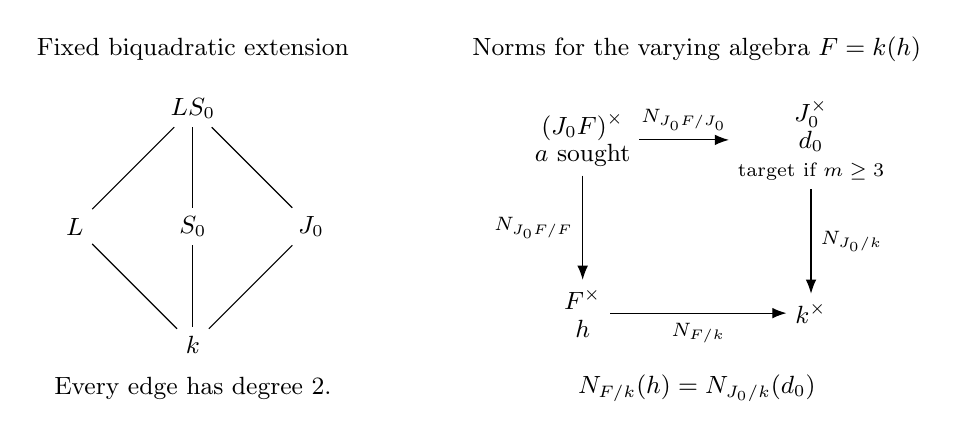
\begin{tikzpicture}[
  font=\small,
  field/.style={inner sep=3pt},
  norm/.style={-{Latex[length=1.8mm]},thin},
  every node/.style={align=center}]
  \begin{scope}[xshift=-3.2cm]
    \node at (0,2.25) {Fixed biquadratic extension};
    \node[field] (top) at (0,1.5) {$LS_0$};
    \node[field] (left) at (-1.5,0) {$L$};
    \node[field] (middle) at (0,0) {$S_0$};
    \node[field] (right) at (1.5,0) {$J_0$};
    \node[field] (bottom) at (0,-1.5) {$k$};
    \draw (top) -- (left) -- (bottom);
    \draw (top) -- (middle) -- (bottom);
    \draw (top) -- (right) -- (bottom);
    \node at (0,-2.05) {Every edge has degree $2$.};
  \end{scope}
  \begin{scope}[xshift=3.2cm]
    \node at (0,2.25) {Norms for the varying algebra $F=k(h)$};
    \node[field] (jf) at (-1.45,1.1)
      {$(J_0F)^\times$\\[-1pt]$a$ sought};
    \node[field] (j) at (1.45,1.1)
      {$J_0^\times$\\[-1pt]$d_0$\\[-1pt]
       {\scriptsize target if $m\geq3$}};
    \node[field] (f) at (-1.45,-1.1)
      {$F^\times$\\[-1pt]$h$};
    \node[field] (k) at (1.45,-1.1)
      {$k^\times$};
    \draw[norm] (jf) -- node[above,font=\scriptsize]
      {$N_{J_0F/J_0}$} (j);
    \draw[norm] (jf) -- node[left,font=\scriptsize]
      {$N_{J_0F/F}$} (f);
    \draw[norm] (j) -- node[right,font=\scriptsize]
      {$N_{J_0/k}$} (k);
    \draw[norm] (f) -- node[below,font=\scriptsize]
      {$N_{F/k}$} (k);
    \node at (0,-2.05) {$N_{F/k}(h)=N_{J_0/k}(d_0)$};
  \end{scope}
\end{tikzpicture}
\caption{The fields and norms in the even-degree factorization.
The left diagram is fixed before $u$ is chosen; its edges denote
field inclusions. On the right, for $u\in\Omega$, the \'etale algebra
$F=k(h)$ has degree $m$ and depends on $u$; here
$J_0F=J_0\otimes_k F$.
The norm square commutes. For $m\geq3$, the sought element $a$
must map to both $h$ and $d_0$; their norms to $k$ already agree.
For $m=2$, only the norm condition to $F$ is imposed at this stage.}
\label{fig:even-degree-norms}
\end{figure}

\FloatBarrier

\subsection{Auxiliary fields for the degree-four correction}
\label{ind:auxiliary-fields}

Suppose in this subsection that $D$ has degree four over $L$.
Retain the Hermitian quadratic field $S_0=k(s)$ already constructed,
put $E=LS_0$ and $C_s=C_D(s)$, and let $J_0$ be the third quadratic
subfield of the biquadratic extension $E/k$.  Thus $C_s$ is a
quaternion algebra over $E$, with a unitary involution over $S_0$.
When its unitary groups are viewed inside the ambient groups over
$k$, restriction of scalars from $S_0$ is understood.
We will correct the determinant of an element of
$\U(C_s,*)\cap S$ by elements in binary special unitary groups.
The auxiliary fields in the following lemma let us prescribe where
those binary groups are split.  This construction is the degree-four
determinant correction of \cite[Section~7]{MPNF}, with separable
quadratic descent used also in characteristic two.

\begin{lemma}\label{ind:auxiliary-fields-lemma}
There is a finite set $B_s$ of places of $k$, depending only on
$(D,*,S_0)$, with the following property.  For every finite set $T$
of places disjoint from $B_s$, there is a separable quadratic field
$F'=k(f)\subset C_s$ such that $f^*=f$, $F'$ is linearly disjoint
from $E$, and, for every $v\in T$,
\[
 F'\otimes_k k_v\simeq k_v\times k_v,
 \qquad
 \SU(C_D(F'),*)\otimes_{F'} F'_w\simeq\SL_2
 \quad\text{for both }w\mid v.
\]
Here $\SU(C_D(F'),*)$ is a group over $F'$: its central simple
algebra has center $LF'$ and degree two.  The embeddings can be
chosen so that $f$ has reduced trace zero in $C_s$ in odd
characteristic, and reduced trace one in characteristic two.
\end{lemma}

\begin{proof}
Write $\kappa$ for canonical quaternion conjugation on $C_s$.
It commutes with $*$, since reduced trace commutes with $*$.
Consequently $*\circ\kappa$ is a semilinear algebra automorphism
of order two relative to $E/S_0$.  Its fixed algebra $B_0$ is a
quaternion algebra over $S_0$, and Galois descent gives
\[
 B_0\otimes_{S_0}E=C_s.
\]
The restriction of $*$ to $B_0$ is canonical conjugation.
This descent is valid in characteristic two as well, because
$E/S_0$ is separable; see \cite{KMRT}.

Fix $B_s$ at this point, containing all places below ramification
of $B_0$ and sufficiently large for the following integral
properties outside $B_s$.  The fields $L$ and $S_0$ are
unramified, the fixed algebras and embeddings have unramified
integral models, and the involution at a nonsplit place of $L/k$
is given, up to scalar, by a unimodular Hermitian form.
When $S_0$ splits, its two orthogonal Hermitian blocks are
unimodular as well.  These properties follow by spreading the
fixed algebras, involution and separable embedding; the local
classification of unitary involutions gives the stated Hermitian
description \cite{KMRT}.

We first construct an abstract quadratic extension that embeds in
$B_0$.  Suppose the characteristic is odd.  Choose
$i_0\in L^\times$ with $\Tr_{L/k}(i_0)=0$.  For a scalar
$c\in k^\times$, consider the quadratic algebra over $S_0$ with
generator $y$ and equation
\[
 y^2=i_0^2c.
\]
An embedding of this algebra in $B_0$ has $y^*=-y$.  The element
$f=y/i_0\in C_s$ therefore satisfies
\[
 f^*=f,\qquad f^2=c,\qquad\Trd_{C_s}(f)=0.
\]
In characteristic two, write
$L=k(\iota)$ with $\iota^2+\iota=b_L\in k$.
Instead use the quadratic algebra over $S_0$ with equation
\[
 y^2+y=c+b_L,\qquad c\in k.
\]
Its generator has reduced trace one, so $y^*=y+1$ in $B_0$.
Then $f=y+\iota$ satisfies
\[
 f^*=f,\qquad f^2+f=c,\qquad\Trd_{C_s}(f)=1.
\]
These formulas specify how a quadratic embedding in $B_0$ produces
a Hermitian quadratic embedding in $C_s$ in either characteristic.

A quadratic separable field over $S_0$ embeds in $B_0$ precisely
when it remains a field at every ramified place of $B_0$.
Indeed a quadratic local field extension kills the invariant
$1/2$ of a quaternion division algebra, whereas the split algebra
does not.  The global Brauer invariant theorem then gives the
splitting, and hence the embedding, criterion
\cite{Reiner,MilneCFT}.
The resulting local conditions on $c$ occur above $B_s$ and
can always be met.
In odd characteristic, the kernel of
\[
 k_v^\times/k_v^{\times2}
 \longrightarrow S_{0,w}^\times/S_{0,w}^{\times2}
\]
has at most two elements when $S_{0,w}/k_v$ is quadratic,
and one when $S_{0,w}=k_v$.  The square-class group of an
odd-characteristic local field has four elements.  We can therefore
choose $c$ so that $i_0^2c$ is nonsquare at each required place.
In characteristic two the same argument applies to the restriction
map on Artin--Schreier classes
\[
 k_v/\{a^2+a:a\in k_v\}
 \longrightarrow
 S_{0,w}/\{a^2+a:a\in S_{0,w}\}.
\]
Its kernel has at most two elements, whereas its source is infinite.
Thus $c+b_L$ can be required to have nonzero image.
If $S_0$ has two places over $v$, both completions equal $k_v$
and the exclusions at those places are identical.

At every $v\in T$, require that $c$ define a split quadratic
algebra over $k_v$: take $c$ to be a nonzero square in odd
characteristic and an Artin--Schreier value in characteristic two.
At one further place $v_*$, split completely in $E$ and outside
$B_s\cup T$, require the quadratic algebra defined by $c$ to be
a field.  Chebotarev supplies $v_*$, and weak approximation supplies
$c$ satisfying all these local conditions.  The conditions are
open in the local fields; for Artin--Schreier classes this follows
also from the surjectivity of $a\mapsto a^2+a$ on the maximal
ideal.  The field $F'$ defined by $c$ is disjoint from $E$:
otherwise it would be one of the three quadratic subfields of
$E$, all of which split at $v_*$.
The associated algebra for $y$ over $S_0$ is therefore a field,
and the embedding criterion gives an embedding in $B_0$.
The preceding formulas give $F'\subset C_s$; moreover $EF'$ is
a field of degree two over $E$, hence a maximal subfield of $C_s$.

We next choose this embedding so that the two binary groups split
at the places in $T$, using the integral properties secured when
$B_s$ was fixed.

Fix $v\in T$ and put $K=k_v$.  When $L$ splits at $v$, the algebra
on each $L$-component is $M_4(K)$.  Put $A_0=S_0\otimes_kK$.
The four-dimensional module is free of rank two over $A_0$,
and its $s$-centralizer is $\operatorname{End}_{A_0}(A_0^2)$.
For the two roots $\lambda_1,\lambda_2\in K$ of the chosen
polynomial of $f$, take $f=\diag(\lambda_1,\lambda_2)$ in
this centralizer.  Its two $K$-eigenspaces are copies of $A_0$,
of dimension two over $K$, whether $A_0$ is a field or split.
Both special groups are $\SL_2$, and the involution specifies
the paired $L$-component.  After splitting $A_0$, each eigenvalue
occurs once in each of the two $s$-blocks, as required.

Suppose instead that $L\otimes_kK$ is the unramified quadratic
field over $K$.  If $S_0$ splits, decompose each of its two
Hermitian blocks into orthogonal lines of unit norm values.
Such decompositions follow by diagonalizing the reduction and
lifting an orthogonal basis, in characteristic two as well.
Assign to each $f$-eigenvalue one line from each $s$-block.
Each resulting binary Hermitian space has unit determinant.
All units of $K$ are norms from the unramified quadratic
extension, so its negative determinant is a norm and the space
is hyperbolic.  Its special unitary group is therefore split.

If $S_0$ is nonsplit, its completion equals the unique unramified
quadratic extension $L\otimes_kK$.  The two $s$-eigenspaces over
that extension are dual totally isotropic two-spaces.
Choose paired bases $e_1,e_2$ and $e'_1,e'_2$ with
$\langle e_i,e'_j\rangle=\delta_{ij}$, and assign one
$f$-eigenvalue to each hyperbolic plane
$\langle e_i,e'_i\rangle$.  This again makes both binary
groups split.

All the local elements $f$ just constructed are Hermitian and
have each eigenvalue once in each $C_s$-block.  They therefore
give local embeddings in $B_0$ by the same descent formulas.
For clarity, in characteristic two $y=f+\iota$ has reduced
trace one and satisfies
\[
 y^*=y+1=\kappa(y),
\]
so it is fixed by $*\circ\kappa$.  Thus it really lies in $B_0$.
In odd characteristic the corresponding identity is
$(i_0f)^*=-i_0f=\kappa(i_0f)$.

Finally, local embeddings of the fixed quadratic algebra for
$y$ are conjugate by $B_0^\times$, by Skolem--Noether.
Weak approximation in the open affine variety $B_0^\times$
over $S_0$ lets a global conjugator approximate all the prescribed
local conjugators.  The splitting property persists under
sufficiently close approximation: the eigenspaces vary
continuously and the determinant norm classes of their Hermitian
forms are locally constant.  The resulting global embedding
has all the asserted properties.
\end{proof}

For each field $F'$ in Lemma~\ref{ind:auxiliary-fields-lemma},
put $G_{F'}=\SU(C_D(F'),*)$, a group over $F'$.
Its restriction of scalars embeds in $S$, since over a separable
closure it acts by special transformations on the two binary
$F'$-eigenspaces.  We will use the inclusion
\begin{equation}\label{ind:binary-norm-inclusion}
 (J_0F'/F')^1\ \subset\
 (\Res_{F'/k}G_{F'}\cap\U(C_s,*))(k),
 \qquad
 \Nrd_{C_s}(b)=N_{J_0F'/J_0}(b).
\end{equation}
Here $(J_0F'/F')^1$ denotes the elements of norm one.
Indeed $EF'$ is a maximal subfield of $C_D(F')$ as well as of
$C_s$.  Its norm to $LF'$ computes the determinant in the
binary algebra; the nontrivial automorphism of $EF'/LF'$
restricts to the nontrivial automorphism of $J_0F'/F'$.
On this last field that automorphism is $*$.
Thus norm one gives both the unitary and special conditions.
The determinant in $C_s$ is the norm from $EF'$ to $E$,
whose restriction to $J_0F'$ is the norm displayed in
Equation~\eqref{ind:binary-norm-inclusion}.

\subsection{Correcting the determinant in degree four}
\label{ind:degree-four}

We now isolate the local conditions on the factor $q$ that suffice
to remove its determinant.  The neighborhoods in the next
proposition are fixed before $q$ is chosen.  This will allow the
preceding factorization to use them as ordinary local
approximation conditions.

\begin{proposition}\label{ind:degree-four-correction}
Assume the Margulis--Platonov assertion for binary special groups
over every finite separable extension of $k$.  Fix the finite
quotient $S(k)/R$, of exponent dividing $e$, and retain the
degree-four data $(D,*,S_0)$ above.  Let $B$ be a nonempty finite
set of places of $k$ containing $B_s$ and all places below the
rank-zero places of the group $\SU(C_s,*)$ over $S_0$.
There are identity neighborhoods $W_v$ in
$(\U(C_s,*)\cap S)(k_v)$, for $v\in B$, such that every
\[
 q\in(\U(C_s,*)\cap S)(k),\qquad q_v\in W_v\quad(v\in B),
\]
has trivial image in $S(k)/R$.
\end{proposition}

\begin{proof}
First fix a field $F_1$ given by
Lemma~\ref{ind:auxiliary-fields-lemma}, with no extra local
prescriptions, and fix its embedding in $C_s$.  Write
$G_i=\SU(C_D(F_i),*)$ when a field $F_i$ has been specified.
The field $F_1$ will remain fixed when the neighborhoods $W_v$
are chosen; a second field $F_2$ will be chosen after $q$.

For an element $q$ in the proposition put
\[
 r_0=\Nrd_{C_s}(q)\in E^\times.
\]
Let $\alpha$ and $\beta$ be the automorphisms of $E/k$ fixing
$S_0$ and $L$, respectively.  Unitarity gives
$\alpha(r_0)=r_0^{-1}$, and ambient determinant one gives
\[
 N_{E/L}(r_0)=1,\qquad\beta(r_0)=r_0^{-1}.
\]
Hence $\alpha\beta$ fixes $r_0$, so $r_0\in J_0^1$.
Write a bar for the nontrivial automorphism of $J_0/k$.
Choose once and for all $c_*\in J_0$ with
$c_*+\bar c_*=1$, and set
\begin{equation}\label{ind:determinant-hilbert90}
 d=c_*+r_0\bar c_*.
\end{equation}
This formula is valid in both characteristics.  It satisfies
$r_0\bar d=d$ and gives $d=1$ when $r_0=1$.
We will require $q$ close enough to $1$ at $B$ that $d$ is
invertible, in which case $r_0=d/\bar d$.

We describe the neighborhoods $W_v$ before making any further
choices.  The local norm map for the fixed separable quadratic
algebra $J_0F_1/J_0$ is a submersion at $1$: its differential is
the surjective trace map, also in characteristic two.
For $d$ sufficiently close to $1$, it therefore has solutions
\begin{equation}\label{ind:first-field-local-norm}
 N_{J_0F_1/J_0}(x_{1,v})=d,\qquad x_{1,v}\longrightarrow1
 \quad\text{as }d\longrightarrow1,
\end{equation}
in the product of the local algebras above $v$.
Because the field and embedding are fixed, the elements
$b_{1,v}=x_{1,v}/x_{1,v}^*$ tend to $1$ in the ambient algebra
$D\otimes_k k_v$.

By the binary case of MP and
Proposition~\ref{arith:finite-quotients}, the quotient maps on
$G_1(F_1)$ and on $\SU(C_s,*)(S_0)$ extend continuously to
their respective products of rank-zero local groups.
Choose $W_v$ so small that the solutions in
Equation~\eqref{ind:first-field-local-norm} make $b_{1,v}$
belong to the needed identity neighborhoods at every rank-zero
place of $G_1$ over $v$.  At the same time require $q$ and
$b_{1,v}$ close enough to $1$ that
\[
 (b_{1,v}b_{2,v})^{-1}q
\]
belongs to the needed identity neighborhoods for
$\SU(C_s,*)$ whenever $b_{2,v}$ is sufficiently close to $1$
and the displayed element has determinant one in $C_s$.
These requirements concern finitely many fixed groups and
continuous multiplication maps, so they hold after shrinking
$W_v$.  They also ensure that $d$ is invertible.
For a later field $F_2$, its local target at every $v\in B$
will be $x_{2,v}=1$.  Once $F_2$ is fixed, approximation to that
target can be made arbitrarily close both in its binary group
and in $D$; no choice of $F_2$ enters the present neighborhoods.

Now let $q$ satisfy these conditions, and hence fix $r_0$ and $d$.
Say that a place $v\notin B$ is covered by $F_i$ if
\begin{enumerate}
\item $d$ is a norm from $J_0F_i/J_0$ at every place of $J_0$
      above $v$; and
\item $G_i$ is isotropic at every place of $F_i$ above $v$.
\end{enumerate}
All but finitely many places are covered by the fixed field $F_1$.
Indeed, away from the ramification and the divisors of $d$, norms
from unramified quadratic algebras are surjective on units.
Also $G_1$ is an unramified binary group at all but finitely many
places, and is split there: a quaternion algebra over a local
field with unramified integral model has trivial Brauer class,
since the residue field is finite.

Let $T$ be the finite set of places outside $B$ not covered by
$F_1$.  Apply Lemma~\ref{ind:auxiliary-fields-lemma} to choose
$F_2$ split at every place of $T$, with both binary groups split
there.  The algebra $J_0F_2/J_0$ is then locally split at every
place over $T$, and its norm is surjective.  Thus every place
outside $B$ is covered by at least one of $F_1,F_2$.

We seek invertible elements $x_i\in J_0F_i$ satisfying
\begin{equation}\label{ind:degree-four-multinorm}
 N_{J_0F_1/J_0}(x_1)N_{J_0F_2/J_0}(x_2)=d.
\end{equation}
At the places above $B$, take the local solutions
$x_1=x_{1,v}$ already specified and $x_2=1$.
At any other $k$-place choose a field covering that entire
place, let its variable carry the norm $d$ at every $J_0$-place
above it, and set the other variable equal to $1$.
This gives local solutions everywhere.
It also arranges the following useful condition: if $G_i$
has a rank-zero place above $v\notin B$, then $F_i$ cannot
cover $v$, so the other field covers it and $x_i=1$ on all
components above $v$.

We justify both the Hasse principle and the required weak
approximation for Equation~\eqref{ind:degree-four-multinorm},
including in characteristic two.  Put $K=J_0$, $E_i=J_0F_i$
and $y_2=x_2^{-1}$.  On the locus where the variables are
invertible the equation becomes
\begin{equation}\label{ind:degree-four-quadric}
 N_{E_1/K}(x_1)-dN_{E_2/K}(y_2)=0.
\end{equation}
Both norm forms are nonsingular binary quadratic forms because
$E_i/K$ is separable; their direct sum in this display is a
nonsingular four-variable quadratic form.  This remains true
in characteristic two, where its polar form is the direct sum
of two nondegenerate alternating forms.  Its projective zero
locus $X_d\subset\bbP^3_K$ is consequently a smooth quadric
surface, becoming $\bbP^1\times\bbP^1$ over a separable
closure.

Here is a local-global argument for this surface that works
uniformly in the characteristic.  Its two rulings determine
a quadratic \'etale algebra $K'/K$.  The automorphisms of
$\bbP^1\times\bbP^1$ act separately on the two factors or
exchange them.  Descent therefore expresses $X_d$ as the
restriction of scalars, from $K'$ to $K$, of a Severi--Brauer
conic over $K'$; when $K'=K\times K$ this means a product of
two such conics.  A local point of $X_d$ supplies points on
the conic at every completion of $K'$.  The Brauer
local-global theorem over the global field $K'$, componentwise
in the split case, makes the conic split.  Hence $X_d(K)$ is
nonempty; see \cite{MilneCFT} for the Brauer theorem.

A smooth quadric surface with a rational point is rational,
by projection from that point.  Its affine cone minus the
vertex is rational as well: over a rational affine open of
the surface the tautological line bundle is trivial, so the
punctured cone is birational to $\bbA^2\times\bbG_m$.
Weak approximation follows on its smooth locus by using such
a rational chart and density of a nonempty Zariski open in
each local smooth variety.  Remove also the two norm-zero
loci.  The local solutions above belong to the resulting
open set; its rational points still approximate any finite
collection of those local solutions.  Inverting $y_2$ returns
the same Hasse principle and weak approximation for
Equation~\eqref{ind:degree-four-multinorm}.

There are only finitely many rank-zero places of $G_1$ and
$G_2$.  Apply this weak approximation at their underlying
$k$-places and at $B$.  At a rank-zero place outside $B$,
the variable belonging to that group has local target $1$,
as arranged above.  Approximate it closely enough that
$x_i/x_i^*$ lies in an identity neighborhood killed by the
continuous extension of the finite quotient on $G_i$.
At $B$, approximate the specified $x_{1,v}$ and $1$ closely
enough to retain all the conditions used in choosing $W_v$,
and also the analogous kernel conditions for $G_2$.

For the resulting global solution set
\[
 b_i=x_i/x_i^*\quad(i=1,2).
\]
Equation~\eqref{ind:binary-norm-inclusion} places $b_i$ in
$(\Res_{F_i/k}G_i\cap\U(C_s,*))(k)$, and the local conditions just imposed
show that both have trivial image in $S(k)/R$.
Their determinants satisfy
\[
 \Nrd_{C_s}(b_1)\Nrd_{C_s}(b_2)
 =\frac{N_{E_1/K}(x_1)N_{E_2/K}(x_2)}
        {\overline{N_{E_1/K}(x_1)N_{E_2/K}(x_2)}}
 =\frac d{\bar d}=r_0.
\]
Thus $q'=(b_1b_2)^{-1}q$ belongs to $\SU(C_s,*)(S_0)$.
At all its rank-zero places it lies in the prescribed kernel
neighborhoods, since those places lie above $B$.
The binary case of MP therefore makes $q'$ trivial in the
quotient as well.  The identity $q=b_1b_2q'$ proves the
proposition.
\end{proof}


\subsection{Local factorizations near the identity}

We return to even degree $n=2m$. For $m=2$,
Proposition~\ref{ind:degree-four-correction} supplies identity neighborhoods
in $\U(C_s)\cap S$ that can be fixed before $q$ is chosen; for $m\geq3$,
the induction hypothesis supplies kernel neighborhoods in the fixed
group $\SU(C_s)$. It remains to choose a representative of each coset in
$V_0/R$ and solve the norm equations so that both factors $w$ and $q$
are killed. We first construct local open sets near $1$ on which the norm
equations are soluble and their solutions make both factors small in the
ambient algebra.

\begin{lemma}\label{ind:local-near-one}
Let $K=k_v$.  Arbitrarily close to $1$ in $S(K)$ there are nonempty
open sets of elements $u\in\Omega(K)$ for which both equations in
\eqref{ind:a-norms} have a solution $a$.  The elements $a,w,q$ may all
be required to lie in any prescribed ambient identity neighborhoods.
The same assertion holds when the second norm equation is omitted.
\end{lemma}

\begin{proof}
Choose $X\in\Lie(S)(K)$ such that the geometric matrix
$X_{+-}X_{-+}$ is invertible and has separable characteristic polynomial.
This is a nonempty Zariski open condition, as is seen in split
coordinates, and the $K$-points of this vector space are Zariski dense.
Smoothness supplies an analytic curve $u(\varepsilon)$ through $1$ with
derivative $X$.  Formula~\eqref{ind:h-block} gives
\[
                    (h-1)/\varepsilon^2
                       \longrightarrow X_{+-}X_{-+}
\]
on one block, with the same characteristic polynomial on the other.
For small nonzero $\varepsilon$, therefore, $u(\varepsilon)\in\Omega$.

Identify the \'etale algebras generated by $(h-1)/\varepsilon^2$ with
the \'etale algebra generated by its limit.  These identifications vary
continuously: the characteristic polynomials have simple roots, and
simple-root lifting, followed by the basis of powers, identifies the
embeddings in the ambient algebra.  The same holds after adjoining
$J_0$.  Under these identifications, $h\to1$ and $d_0\to1$.

Consider the simultaneous norm map from $(J_0F)^\times$ to the torus of
pairs $(h,d_0)$ satisfying \eqref{ind:norm-compatible}.  This map is
smooth and surjective as a morphism of tori.  Indeed over a splitting
field, write the coordinates of $a$ as $(a_i,b_i)_{1\leq i\leq m}$;
then the map records
\[
           h_i=a_i b_i,\qquad d_+=\prod_i a_i,\qquad
           d_-=\prod_i b_i,\qquad \prod_i h_i=d_+d_-.
\]
Its kernel is the torus $b_i=a_i^{-1}$, $\prod_i a_i=1$, of dimension
$m-1$.  There is no inseparability in this assertion, even when the
characteristic divides $m$.  The local submersion theorem supplies
solutions $a\to1$.  Formula~\eqref{ind:two-factors} then gives $w,q\to1$.
If only the first norm is specified, the same argument uses the ordinary
quadratic norm map.  Around any sufficiently small fixed nonzero
$\varepsilon$, these properties persist on an open set, by the same
continuous \'etale identifications and norm submersion.
\end{proof}

At auxiliary places split in $LS_0$ and in $D$, these neighborhoods can
also prescribe a Frobenius cycle type for $\Psi$.  In split coordinates
take
\begin{equation}\label{ind:cycle-model}
 u=\begin{pmatrix}I&\varepsilon I\\
                  \varepsilon X&I+\varepsilon^2X\end{pmatrix}.
\end{equation}
Its determinant is one and $h_+=I+\varepsilon^2X$.  Choose $X$ integral
with invertible separable residue characteristic polynomial of the
specified factorization type.  At sufficiently large residue fields
all cycle types are available.  Taking $\varepsilon$ small gives the
norm solutions and smallness of Lemma~\ref{ind:local-near-one} while
retaining that type for the \'etale field generated by $h$.

\subsection{The approximation conditions for the even step}

Assume the induction hypothesis in degrees smaller than $2m$.  We will
choose a representative $u$ of an arbitrary coset in $V_0/R$ for which
Lemma~\ref{ind:even-factorization} can be applied globally.  The choice
must control the anisotropic places of the variable quaternion algebra
$Q$, as well as the fixed group $\SU(C_s)$.

Choose a finite set $B$ containing $A$, the places below the anisotropic
places of $\SU(C_s)$, all exceptions to integral models of the fixed
data, and an isotropic place $v_0$ of $S$.  In degree four include $B_s$
and apply Proposition~\ref{ind:degree-four-correction} at this point.
Denote this set by $B_{\mathrm{corr}}$; its field $F_1$ and neighborhoods
$W_v$, $v\in B_{\mathrm{corr}}$, are now fixed.  Subsequent enlargements
of $B$ retain those neighborhoods on $B_{\mathrm{corr}}$ and impose
no additional determinant-correction condition.  At every added place
we may still choose near-identity openings using
Lemma~\ref{ind:local-near-one}.

Enlarge $B$ by sufficiently large auxiliary places split in $LS_0$
and in $D$ at which we impose,
using \eqref{ind:cycle-model}, every permutation cycle type of degree
$m$.  These conditions force the splitting field of $\Psi$ over
$LS_0$ to have group $S_m$.  To recall the group-theoretic argument,
the transitive $S_m$-action on the cosets of a proper subgroup has
a derangement, as follows by averaging the numbers of fixed points.
An element conjugate into that subgroup fixes a coset, so the
derangement's conjugacy class misses the subgroup.  A subgroup
containing every cycle type therefore cannot be proper.

At each place of $B$, use Lemma~\ref{ind:local-near-one}.  Require $u$
to lie sufficiently near $1$ that its $A$-coordinate belongs to $P_0$;
then these openings are compatible with every coset in $V_0/R$ by
Proposition~\ref{arith:closure}.  Require $w$ to be small enough for
Lemma~\ref{ind:binary-smallness}.  When $m\geq3$, require $q$ to be
small enough to be killed in the fixed smaller group $\SU(C_s)$.
When $m=2$, require $q_v\in W_v$ for
$v\in B_{\mathrm{corr}}$; at the other places of $B$ we may require
any sufficiently small identity neighborhood.

Outside $B$ we allow either $u\notin\Omega$, or a point $u\in\Omega$
for which the required norm equations are soluble and $Q$ is split at
every local factor of $F$.  We also allow a nonempty open set near $1$
from Lemma~\ref{ind:local-near-one}, where the norm equations are
soluble and $w$ is small enough for
Lemma~\ref{ind:binary-smallness}; this second open set will only be used
at the denominator places $B_1$ introduced in
Proposition~\ref{approx:power-factor}.  Once such a place is known, we
choose an indicated local solution $a$ there.  No extra condition on
$q$ is needed outside $B$, because all anisotropic places of the fixed
group lie above $B$.

We verify the two remaining hypotheses of the approximation
proposition: a codimension-two exclusion at integral reductions and
nonempty algebraic tests at a single pole.  This will ensure that the
only nonsplit quaternion factors occur above $B\cup B_1$, where their
elements are already small.

\subsubsection{Integral reduction}

Over a splitting field consider the four divisors
\[
          \det A'=0,\qquad\det B'=0,\qquad
          \det C'=0,\qquad\det D'=0
\]
in the split matrix group.  Exclude their pairwise intersections.  If
$m\geq3$, impose also the following conditions.  Off all four divisors,
$\Psi$ must have at least one simple absolute root.  On one divisor
alone, require $0$ to be a simple root for a diagonal divisor, and $1$
to be a simple root for an off-diagonal divisor.  The asserted root
already occurs by the complementary-minor identities; for example
\[
 1-A'(u^{-1})_{++}=B'(u^{-1})_{-+}.
\]
For $m=2$ there is no simple-root requirement.

These exclusions are invariant under descent.  Exchanging $s$-labels
interchanges the two diagonal divisors and the two off-diagonal
divisors.  The unitary diagram action does the same, because it acts
by inverse transpose and complementary minors.  More explicitly,
the automorphisms of $LS_0/k$ fixing $L$ and $S_0$ each interchange
both pairs, while their product fixes each divisor.  The permutation
character on either pair is therefore the quadratic character of
$J_0/k$.  The excluded closures define a $k$-subvariety $Y$.

We claim that $Y$ has geometric codimension at least two.  Work first
in $\GL_{2m}$.  The four determinant hypersurfaces are distinct and
irreducible, so their pairwise intersections have codimension at least
two.  On each one, the simple-root requirement holds generically: use
independent two-dimensional transformations on $m$ pairs, with one
line in each block, and arrange exactly one of the resulting values
to be $0$ or $1$.  Off the divisors the matrix
$B'D'^{-1}C'A'^{-1}$ is a submersive parameter.  For $m\geq3$, matrices
with no simple characteristic root have codimension at least two.
Indeed their distinct eigenvalues have at most $\lfloor m/2\rfloor$
parameters, and each Jordan orbit has dimension at most $m^2-m$.
The resulting dimension is at most $m^2-2$.  Finally all these tests
are invariant under scalar multiplication of $u$, which carries the
codimension statement to $\SL_{2m}$.  Enlarge $B$ to make these
statements valid on the integral models.

Let an integral point reduce outside $Y$, and assume it belongs to
$\Omega$.  If $J_0$ is nonsplit at this place, its Frobenius interchanges
both pairs of divisors.  A rational residue point lying on one divisor
would therefore lie on its mate, which is excluded.  Thus it lies on
none, and $h$ and $1-h$ are units in every local factor of $F$.  The
quadratic extension defined by $J_0$ is unramified, so $-h(1-h)$ and
$h$ are norms of units.  This proves that $Q$ is split and gives a unit
solution of the first equation in \eqref{ind:a-norms}.

For $m\geq3$ the second equation can be imposed as well.  Given a unit
solution of the first, its determinant discrepancy is a norm-one unit
in $J_0$.  A simple residue root of $\Psi$ gives an unramified factor of
$F$ over the local ground field.  Write the discrepancy as $y/\bar y$
by Hilbert~90, taking $y$ a unit; its valuation can be removed by a
ground-field uniformizer.  The norm on units from that unramified
factor, after extending to $J_0$, is surjective.  Lift $y$ through that
norm and divide the lift by its conjugate.  This changes the second
norm by the required discrepancy without changing the first.

If $J_0$ splits, the quaternion algebra is split and the first equation
is immediate.  For the second equation, identify $J_0$ with two copies
of the local field.  Choose the first component of $a$ with prescribed
norm equal to the first component of $d_0$, and determine the other
component from $h$; compatibility \eqref{ind:norm-compatible} gives its
correct norm.  Off the divisors, the prescribed norm is a unit and the
simple residue root again supplies an unramified factor.  On one
divisor, the simple residue root $0$ or $1$ lifts to a degree-one factor
of $F$, whose norm has no restriction on valuation.  This proves all
required local assertions for integral points reducing outside $Y$.

\subsubsection{A single pole}

Take the fixed Galois field $M$ in
Proposition~\ref{approx:power-factor} large enough to split all fixed
data.  A single pole then occurs only at a place split completely in
$M$.  In degree four, $J_0$ is consequently split, so there is no
additional pole condition.  For $m\geq3$, it is enough to force $\Psi$
to split, which makes both norm equations soluble.

Order the cocharacter exponents as $d_1<\cdots<d_{2m}$.  At a single
pole the split matrix expression is
\[
 u=g_L\diag(t^{ed_1},\ldots,t^{ed_{2m}})g_R,
\]
with integral invertible side factors and $\ord(t)>0$.  For the $b$-th
elementary coefficient of $\Psi$, $1\leq b\leq m$, require
\begin{equation}\label{ind:pole-valuations}
 \ord(c_b(\Psi))=e\,\ord(t)
                   \sum_{j=1}^b(d_j-d_{2m+1-j}).
\end{equation}
These equalities follow from finitely many nonvanishing minor tests.
Indeed write the coefficient as the exterior trace for
$P u P u^{-1}P$.  The uniquely lowest-weight term uses the first $b$
indices in the positive exterior power and the last $b$ in the inverse.
Its coefficient is a product of opposite minors in the two rank-$m$
projections
\[
                    g_R P g_R^{-1},\qquad g_L^{-1}P g_L.
\]
Requiring these minors to be nonzero on reduction gives
\eqref{ind:pole-valuations}.  Such minors are generically nonzero on
the variety of projections: one may use complementary subspaces in
general position, or independent two-dimensional projections on the
paired coordinates.  The successive differences of the displayed
valuations are strictly ordered.  Every segment of the Newton polygon
therefore has length one, and $\Psi$ splits over the local field.

We must also check the order of the generic choices in
Proposition~\ref{approx:power-factor}.  On the hyperplane belonging to a
factor with conjugator $k_j$, put all other parameters equal to $1$.
Then, in the corresponding fixed bases, $g_R=k_j^{-1}$ and $g_L=xk_j$,
where $x$ is the initial rational point.  For the two basic lists first
choose the conjugators so that the right-hand minor tests hold.  Next
choose $x$, subject also to the prescribed local openings, so that all
left-hand tests hold.  These are finitely many nonempty Zariski open
conditions.  For every appended conjugator, $x$ has already been fixed;
both conditions are still nonempty open conditions on that conjugator,
since conjugation sweeps out the full variety of rank-$m$ projections.
Impose the tests also on all Galois-conjugate hyperplanes.  They form one
finite algebraic family independent of the place, and inserting identity
parameters in appended factors preserves all earlier tests.  This is
exactly the pole hypothesis of the approximation proposition.

\subsubsection{Choosing the representative and solving the norms}

All hypotheses of Proposition~\ref{approx:power-factor} are now verified.
Apply it to a prescribed coset in $V_0/R$ and the local openings at $B$.
At the finite set $B_1$ of denominator places of its initial point, use
the near-identity open sets already described, with local solutions
$a$ making $w$ sufficiently small.  At any further model or projection
exceptions introduced in the proof of that proposition, use the
integral-reduction open sets supplied by its original basic list.
These later places therefore introduce no additional nonsplit
quaternion factors requiring smallness.  We obtain $u$ in the
prescribed coset, with
\[
 u\in\Omega,\qquad \Gal(\Psi/LS_0)=S_m,
\]
with all required norm equations locally soluble, and with $Q$ split
outside $B\cup B_1$.

The Galois condition implies that $F=k(h)$ is a field.  If $\widetilde F$
is its splitting field over $k$, then
$\Gal(\widetilde F/k)\subset S_m$ already contains
$\Gal(\widetilde F LS_0/LS_0)=S_m$.  Thus this group is $S_m$ and
$\widetilde F\cap LS_0=k$.  In particular the pair $F,J_0$ has the
joint group required by Proposition~\ref{tor:norm-approximation}.

For $m\geq3$, apply that theorem to \eqref{ind:a-norms}, using
\eqref{ind:norm-compatible}.  It gives a global $a$ approximating the
selected local solutions at $B\cup B_1$.  The binary factor $w$ is
killed: its quaternion algebra is split away from these places, and
at every anisotropic factor above them its eigenvalues satisfy
Lemma~\ref{ind:binary-smallness}.  The factor $q\in\SU(C_s)$ is killed
by the induction hypothesis and its smallness at the anisotropic
places of this fixed degree-$m$ group.  Hence $u=wq$ is killed.

For $m=2$, the first equation of \eqref{ind:a-norms} is a cyclic norm
equation over $F$.  The Hasse norm theorem gives a global solution \cite{MilneCFT}.
Its solution variety is a torsor under the norm-one torus of a
separable quadratic extension; after choosing a solution this torus
is rational, so it has weak approximation.  We may therefore approximate
all selected local solutions at $B\cup B_1$.  The binary factor $w$
is killed by the same argument, and $q\in\U(C_s)\cap S$ lies in the
neighborhoods fixed in Proposition~\ref{ind:degree-four-correction}.
That proposition kills $q$ as well.  This completes the even step.

\begin{proof}[Proof of Theorem~\ref{ind:main}]
Proceed by induction on the degree, simultaneously over all global
function fields.  The inner and isotropic cases supply the base and
all instances of those types.  The odd-degree argument proves the
assertion directly in division degree and by smaller plane groups
otherwise.  In even degree the preceding construction kills a
representative of each coset in $V_0/R$, and hence $V_0/R=1$.

To justify the form of the induction hypothesis used for smaller
groups, recall that vanishing of the power defect for every $e$
already gives their Margulis--Platonov assertion.  A noncentral normal
subgroup has finite index by Lemma~\ref{arith:finite-index};
choosing $e$ to kill the finite quotient puts the generated power
subgroup inside it.  The equality $V_0=R$ makes this power subgroup
open for the topology from the anisotropic places.  A subgroup
containing it is open and, by density, is the inverse image of its
open normal closure.  Thus each completed degree supplies precisely
the hypothesis used in the next degree, including over finite
separable extensions of $k$.
\end{proof}

\section{Proof of the main theorem}\label{sec:conclusion}

\begin{proof}[Proof of \cref{thm:main}]
The global Kneser--Tits theorem handles the isotropic case, and the known
inner-type-$A$ theorem handles anisotropic inner forms.  As explained in
\cref{sec:arithmetic}, Harder's theorem leaves only the anisotropic
unitary groups $S=\SU(D,*)$ of degree $n\geq3$.

Let $N\triangleleft S(k)$ be noncentral.  By
\cref{arith:finite-index}, the group $S(k)/N$ is finite.  Choose an integer
$e\geq1$ divisible by its exponent.  With the notation
\eqref{arith:power-notation}, we have $R\subset N$, while
\cref{ind:main} gives
\[
 R=V_0=\delta_A^{-1}(P_0).
\]
Thus $N$ is a union of cosets of the open subgroup
$\delta_A^{-1}(P_0)$.  More explicitly, density of $\delta_A(S(k))$
induces an isomorphism of finite groups
\[
 S(k)/R\ \simeq\ H_A/P_0.
\]
Let $W$ be the inverse image in $H_A$ of the normal subgroup corresponding
to $N/R$.  Then $W$ is open and normal, and
$N=\delta_A^{-1}(W)$.  Density also shows that
$W=\overline{\delta_A(N)}$, so this local subgroup is uniquely determined
by $N$.  If $A$ is empty, $H_A$ is trivial and the same argument gives
$N=S(k)$.
\end{proof}

\appendix
\section{The finite simple-group obstruction}\label{sec:finite-groups}

We prove Theorem~\ref{fin:obstruction}, following the finite-group
argument of \cite[Section~6]{MPNF}. In addition to the double-coset
obstruction proved there, we verify for each constructed set that its
complement in an abelian subgroup meeting it is a subgroup. In
characteristic two, this property supplies the finite abelian quotient
used in Proposition~\ref{rec:two}. The resulting functions have additive
period groups of finite index, which rules out the exceptional points
left by the density argument.

The proof uses the classification of finite simple groups
\cite[Classification Theorem, p.~737]{Aschbacher2004}. Its common
mechanism is to locate a part of a commuting pair on which centralizers
are small. For alternating and linear groups, this part consists of two
points or a line and a hyperplane. For the remaining classical groups it
is a large irreducible subspace. Most exceptional and sporadic groups
instead have an abelian subgroup whose nonidentity elements have exactly
that subgroup as centralizer. We first establish the two elementary tests
behind these constructions.

Throughout this section, $\mathcal F$ is a finite nonabelian simple group,
$C(B)=C_{\mathcal F}(B)$, and
\[
 I(\mathcal F)=\{g\in\mathcal F:g^2=1\},\qquad
 k(\mathcal F)=\text{the number of conjugacy classes of }\mathcal F.
\]
For commuting $W,Z\in\mathcal F$, the condition to be excluded is
\begin{equation}\label{fg:relation}
 ZW\in C(B)(ZW^{-1})C(BZ^2)
 \quad\text{for every }B\in\mathcal F.
\end{equation}
The choice of the nonempty proper conjugacy-invariant set $\mathcal S$
will be specified in each family. For every choice we must prove both
that Equation~\eqref{fg:relation} fails for some $B$ whenever
$W\in\mathcal S$ and $Z\notin\mathcal S$ commute, and that the
complement condition in Theorem~\ref{fin:obstruction}(ii) holds.

\subsection{Two elementary tests}

First take
\begin{equation}\label{fg:square-set}
 \mathcal S=\{W\in\mathcal F:W^2\ne1\}.
\end{equation}
This set is nonempty, since a group of exponent two is abelian, and it
does not contain the identity. For every abelian subgroup $A$, its
complement is the subgroup $A[2]=\{a\in A:a^2=1\}$. Thus this choice
automatically satisfies Theorem~\ref{fin:obstruction}(ii). For commuting $W\in\mathcal S$ and
$Z\notin\mathcal S$, put $v=ZW$. Then $Z^2=1$, $v^2=W^2\ne1$, and
Equation~\eqref{fg:relation} becomes
\begin{equation}\label{fg:inverse-coset}
 v\in C(B)v^{-1}C(B)\quad\text{for every }B\in\mathcal F.
\end{equation}
Suppose that $\mathcal F$ acts on a set and that some point $p$ satisfies
$v^2p\ne p$. If $C(B)$ fixes $p$ and $vp$ pointwise, writing
$v=a v^{-1}b$ with $a,b\in C(B)$ gives
$vp=a v^{-1}p$. Applying $a^{-1}$ gives $vp=v^{-1}p$, a contradiction.
We call this the point-pair test. We will also use its incidence version:
if $C(B)$ fixes a line $p$ and preserves a subspace $L$, while $vp\subset L$
and $v^{-1}p\not\subset L$, the same equation is impossible.

The second test uses a self-centralizing abelian subgroup.
\begin{lemma}\label{fg:abelian-test}
Suppose that $C\subset\mathcal F$ is an abelian subgroup of odd order
$c>1$ such that $C_{\mathcal F}(t)=C$ for every $1\ne t\in C$. If
\begin{equation}\label{fg:class-bound}
 |\mathcal F|>k(\mathcal F)c^4,
\end{equation}
then the union $\mathcal S$ of the conjugates of $C\setminus\{1\}$
satisfies both assertions of Theorem~\ref{fin:obstruction}.
\end{lemma}
\begin{proof}
The set is nonempty and excludes the identity. If $W\in\mathcal S$ and
$Z$ commutes with $W$, then $Z$ lies in the same conjugate of $C$ as $W$.
Consequently $Z\notin\mathcal S$ forces $Z=1$. More generally,
if an abelian subgroup $A$ meets $\mathcal S$, conjugating one member of
$A\cap\mathcal S$ into $C$ puts all of $A$ in $C$; hence
$A\setminus\mathcal S=\{1\}$. This proves the complement assertion.

Conjugate $W$ into $C$. Testing Equation~\eqref{fg:inverse-coset}
with every conjugate of a fixed nonidentity element of $C$ shows that
every conjugate $v$ of $W$ belongs to $Cv^{-1}C$. If
$v=a v^{-1}b$, $a,b\in C$, then
\[
 (v b^{-1})^2=a b^{-1}\in C.
\]
If this square is nonidentity, $v b^{-1}$ centralizes a nonidentity
element of $C$, so $v\in C$. Otherwise $v\in I(\mathcal F)C$.
Since $I(\mathcal F)$ is conjugacy-invariant, $I(\mathcal F)C=CI(\mathcal F)$.
Thus the whole conjugacy class of $W$ lies in $CI(\mathcal F)$, and
\[
 \frac{|\mathcal F|}{c}\le c|I(\mathcal F)|.
\]
The Frobenius--Schur formula and Cauchy--Schwarz give
\[
 |I(\mathcal F)|
 =\sum_{\chi\in\operatorname{Irr}(\mathcal F)}\nu_2(\chi)\chi(1)
 \le\sum_\chi\chi(1)
 \le\sqrt{k(\mathcal F)|\mathcal F|}.
\]
These inequalities contradict Equation~\eqref{fg:class-bound}.
\end{proof}

\subsection{Alternating, linear, and sporadic groups}

For alternating and projective special linear groups we use
Equation~\eqref{fg:square-set}. In $A_n$, choose $p$ with
$v^2p\ne p$. There is an even permutation $B$ fixing exactly $p,vp$
and having distinct odd cycle lengths greater than one on the remaining
points, except when $n=6$ or $8$. Indeed, for odd $n$ use the single
cycle of length $n-2$, and for even $n\ge10$ use lengths $3,n-5$.
Every permutation centralizing these moving cycles is even on their
support. Therefore a centralizer element in $A_n$ cannot interchange the
two fixed points. The point-pair test applies. The two exceptions are
$A_6\simeq\PSL_2(9)$ and $A_8\simeq\PSL_4(2)$.

Now let $\mathcal F=\PSL_l(q)$, $l\ge3$. Choose a line $p$ such that
$v^2p\ne p$. The three lines $p,vp,v^{-1}p$ are distinct. A hyperplane
$L$ can be chosen to contain $vp$ and contain neither $p$ nor $v^{-1}p$:
in the quotient by $vp$, choose a linear functional nonzero on both
remaining nonzero vectors. The union of two proper hyperplanes in the
dual is not the entire dual, also over $\bbF_2$.

On the direct sum $p\oplus L$, take $B$ to be the identity on $p$ and
an irreducible norm-one field multiplication on $L$. Such an element
exists in the cyclic group of order $(q^{l-1}-1)/(q-1)$: a generator
cannot lie in a proper subfield, since that group's order exceeds
$q^{(l-1)/2}-1$ when $l-1\ge2$. A projective centralizer of $B$ is an
actual centralizer. Indeed, scalar multiplication must preserve its
unique base-field eigenvalue, which is $1$, and hence the multiplier is
$1$. The centralizer fixes $p$ and preserves $L$, contradicting the
incidence version of Equation~\eqref{fg:inverse-coset}.

For simple $\PSL_2(q)$, the pointwise stabilizer of two points of the
projective line is a split torus. It contains an element whose
centralizer fixes both points, unless $q=5$: its order is $q-1$ for
even $q$ and $(q-1)/2$ for odd $q$, and a noninvolution in it is regular
with that torus as centralizer. The case $q=5$ is $A_5$. Choosing the
torus for $p,vp$ proves the assertion in all these cases.

For the sporadic groups other than $M_{12}$, and also for the Tits group,
Table~\ref{fg:table-sporadic} gives a prime $c$ for which a cyclic
subgroup of order $c$ is the centralizer of each of its nonidentity
elements. The centralizer orders, class numbers, and group orders are
those in the \emph{Atlas} and the online \emph{ATLAS of Finite Group
Representations}~\cite{Atlas,AtlasOnline}. In each row, an element $x$
in the class labeled $c\mathrm A$ in that group's conjugacy-class table
has $C(x)=\langle x\rangle$ of order $c$. Since $c$ is prime, every
nonidentity power of $x$ has the same centralizer.
The displayed $k$ is the exact class number. In every row the group
order exceeds $kc^4$, so Lemma~\ref{fg:abelian-test} applies.
For example, the smallest margin is $10\cdot5^4=6250<7920=|M_{11}|$.
One may also check the other inequalities using $k\le200$, except that
$k\le25$ suffices for $M_{22},M_{23},J_1$.

\begin{table}[htbp]
\centering
\small
\begin{tabular}{lrr@{\qquad}lrr}
\toprule
Group & $c$ & $k$ & Group & $c$ & $k$\\
\midrule
$M_{11}$ & 5 & 10 & $\mathrm{O'N}$ & 31 & 30\\
$M_{22}$ & 11 & 12 & $\mathrm{Co}_1$ & 23 & 101\\
$M_{23}$ & 23 & 17 & $\mathrm{Co}_2$ & 23 & 60\\
$M_{24}$ & 23 & 26 & $\mathrm{Co}_3$ & 23 & 42\\
$J_1$ & 7 & 15 & $\mathrm{Fi}_{22}$ & 13 & 65\\
$J_2$ & 7 & 21 & $\mathrm{Fi}_{23}$ & 23 & 98\\
$J_3$ & 19 & 21 & $\mathrm{Fi}_{24}'$ & 29 & 108\\
$J_4$ & 43 & 62 & $\mathrm{HN}$ & 19 & 54\\
$\mathrm{HS}$ & 11 & 24 & $\mathrm{Ly}$ & 67 & 53\\
$\mathrm{McL}$ & 11 & 24 & $\mathrm{Th}$ & 31 & 48\\
$\mathrm{He}$ & 17 & 33 & $\mathbb B$ & 47 & 184\\
$\mathrm{Ru}$ & 29 & 36 & $\mathbb M$ & 71 & 194\\
$\mathrm{Suz}$ & 13 & 43 & ${}^2F_4(2)'$ & 13 & 22\\
\bottomrule
\end{tabular}
\caption{Self-centralizing prime-order subgroups for the sporadic and
Tits groups.}\label{fg:table-sporadic}
\end{table}

For $M_{12}$ use its sharply $5$-transitive action of degree $12$ and
the \emph{Atlas} class $8B$, of cycle shape $1^2\,2\,8$
\cite{Atlas,AtlasOnline}; the online database labels this permutation
representation $12a$ (the other degree-$12$ action interchanges the
classes $8A$ and $8B$).
An element centralizing $B\in8B$ restricts to a cyclic shift on its
eight-point orbit. This restriction is injective: its kernel fixes
eight points, and an element fixing five points is the identity.
The centralizer is therefore exactly $\langle B\rangle$, and fixes
the two fixed points individually. Two-transitivity moves this pair to
$p,vp$, so the point-pair test applies with
Equation~\eqref{fg:square-set}.

\subsection{An auxiliary unitary count}

The remaining classical groups need a torus argument on a large
irreducible block. The relevant obstruction takes place in the full
unitary isometry group, which need not itself be simple.

\Needspace{9\baselineskip}
\begin{lemma}\label{fg:unitary-count}
Let $p\ge3$ be an odd prime, let $H=\U_p(q)$ be the full isometry
group of a nondegenerate Hermitian form over $\bbF_{q^2}$, and let
$T\subset H$ be an irreducible torus of order $q^p+1$. If $w\in T$
has field degree $p$ over $\bbF_{q^2}$, then
\[
 w\in T^h w^{-1}T^h\quad\text{for every }h\in H
\]
is impossible.
\end{lemma}
\begin{proof}
Put
\[
 \overline H=H/Z(H),\qquad \overline T=T/Z(H),\qquad
 c=\frac{q^p+1}{q+1},\qquad d=(p,q+1).
\]
The actual centralizer of $w$ is $T$. If $g$ centralizes its projective
image, then $gwg^{-1}=\lambda w$ for a scalar $\lambda$ of norm one.
Taking determinants gives $\lambda^p=1$, so
\begin{equation}\label{fg:unitary-centralizer}
 |C_{\overline H}(\overline w)|\le dc.
\end{equation}

Suppose the displayed condition in the lemma holds. Every conjugate
$v$ of $w$ then lies in $Tv^{-1}T$. The calculation used in
Lemma~\ref{fg:abelian-test} gives an element $u=v b^{-1}$ whose
square lies in $T$. If $u^2$ is nonscalar, it has field degree $p$,
because $p$ is prime; its centralizer is $T$, and hence $u\in T$.
If $u^2$ is scalar, $\overline u$ has square one. Consequently the
entire projective conjugacy class of $\overline w$ lies in
$\overline T I(\overline H)$.

The determinant quotient of $\overline H$ has order $d$, and
$\overline T$ maps onto it. To see this, write $T$ as the norm-one
subgroup of $\bbF_{q^{2p}}^\times$ over $\bbF_{q^p}$. The determinant
of a field multiplication is its norm to $\bbF_{q^2}$. On this torus,
that norm takes a generator to a generator of the scalar norm-one
group of order $q+1$; its exponent is congruent to $c$ modulo
$q^p+1$. Modding out by scalar matrices mods the determinant out by
$p$th powers, giving the quotient of order $d$.

All members of the conjugacy class have the same determinant in this
quotient. For each fixed $i\in I(\overline H)$, at most $c/d$ elements
$t\in\overline T$ have $ti$ with that determinant. Combining this
with Equation~\eqref{fg:unitary-centralizer} gives
\[
 \frac{|\overline H|}{dc}
 \le \frac c d |I(\overline H)|,
 \qquad\text{and therefore}\qquad
 |\overline H|\le c^2|I(\overline H)|.
\]
We show that the reverse strict inequality always holds.

Every projective involution lifts to an involution in $H$. Indeed,
if $g^2=\alpha I$, then $\alpha^p=\det(g)^2$ in the scalar cyclic
group of order $q+1$. As $p$ is odd, $\alpha$ is a square in that
group, and scalar rescaling gives an involution.

For odd $q$, an involution is determined up to conjugacy by the
dimensions $a,p-a$ of its two nondegenerate eigenspaces. Projectively
the unordered partitions are indexed by $1\le a<p/2$, and their
centralizers have order at least
\begin{equation}\label{fg:unitary-odd-centralizer}
 \frac{|\U_a(q)|\,|\U_{p-a}(q)|}{q+1}.
\end{equation}
For even $q$, the Jordan type is $2^a1^b$, where $b=p-2a$. Its full
unitary centralizer has order
\begin{equation}\label{fg:unitary-even-centralizer}
 q^{a^2+2ab}|\U_a(q)|\,|\U_b(q)|.
\end{equation}
We recall the structure behind this formula, including in characteristic
two; see also \cite[Section~2.6, Case~(A)(ii),(iv), pp.~34--36]{Wall1963}.
In the ambient general
linear group the connected matrix centralizer has reductive quotient
$\GL_a\times\GL_b$ and unipotent radical of dimension $a^2+2ab$.
The Hermitian Frobenius gives the unitary forms on both multiplicity
spaces. Equivalently, for $g=1+N$ of order two, $N=N^*$; the induced
forms on $\ker N/\im N$ and, using $N$, on the quotient by $\ker N$
are the forms on these two spaces. Nondegenerate Hermitian forms of
a given dimension over a finite field are isometric. Connectedness
and Lang's theorem give one full-unitary class for each occurring
type and the stated order. Dividing by $q+1$ gives a lower bound
for its projective centralizer.

The unitary order formula implies
\begin{equation}\label{fg:unitary-order-lower}
 |\U_j(q)|=q^{j^2}\prod_{r=1}^j(1-(-q)^{-r})\ge q^{j^2}.
\end{equation}
For completeness, pair consecutive factors: their product is
\[
 (1+q^{-(2r-1)})(1-q^{-2r})
 =1+q^{-2r}(q-1-q^{-(2r-1)})>1.
\]
An unpaired final factor also exceeds one. Thus every nonidentity
projective involution class has centralizer order at least
\[
 M=\frac{q^{(p^2+1)/2}}{q+1}.
\]
There are at most $(p-1)/2$ such classes, and including the identity
gives
\[
 \frac{|I(\overline H)|}{|\overline H|}\le\frac{p+1}{2M}.
\]
When $p\ge5$, we have $c<q^{p-1}$ and
\[
 \frac{M}{q^{2p-2}}
 =\frac{q^{(p^2-4p+5)/2}}{q+1}
 \ge\frac{2^p}{3}>\frac{p+1}{2}.
\]
The first inequality uses $(p^2-4p+5)/2\ge p$ and monotonicity in
$q\ge2$. This proves $c^2|I(\overline H)|<|\overline H|$.

It remains to check $p=3$. Now
\[
 c=q^2-q+1,\qquad h=|\overline H|=q^3(q^3+1)(q^2-1).
\]
There is one nonidentity involution class. In odd characteristic its
centralizer lower bound is $M=q(q-1)(q+1)^2$, and $h/M=q^2c$.
In even characteristic it is $M=q^3(q+1)$, and $h/M=(q^2-1)c$.
In both cases $|I(\overline H)|\le1+q^2c$, whereas
\[
 h-c^2(1+q^2c)
 =c\bigl((3q-4)q^4+(q-2)q^2+q-1\bigr)>0
 \quad(q\ge2).
\]
This includes $\U_3(2)$ and finishes the proof.
\end{proof}

\subsection{Symplectic and orthogonal groups}

Let $\mathcal F$ be a projective symplectic or orthogonal simple group
on its natural space of dimension $2l$ or $2l+1$. We first treat
$l\ge3$, using the standard low-rank identifications and treating
$\PSp_4$ separately below. Choose an odd prime
\begin{equation}\label{fg:block-prime}
 l/2<p\le l,
\end{equation}
requiring $p<l$ in plus orthogonal type. For $l\ge4$, set
$m=\lfloor l/2\rfloor\ge2$. Bertrand's postulate gives
$m<p<2m$, hence $l/2<p<l$, and this prime is odd.
For $l=3$ take $p=3$, apart from plus type, which is $\PSL_4$ and
has already been treated. In odd-dimensional orthogonal type we may
assume odd characteristic, since in even characteristic the group
has the corresponding symplectic realization.

We use a nondegenerate block $E$ of dimension $2p$ carrying a torus
of order $q^p+1$. In orthogonal type this block has minus type; the
complement can be chosen with the sign needed for the ambient form.
For minus type $p=l$ the block is the whole space, whereas the
requirement $p<l$ in plus type leaves a complement of the necessary
sign. The torus is the norm-one subgroup of
$\bbF_{q^{2p}}^\times$ over $\bbF_{q^p}$, acting on $E$ by field
multiplication.

Define $\mathcal S$ to consist of those projective elements whose
square, on the natural space, has an irreducible self-dual block of
dimension $2p$. This condition is independent of the choice of a
scalar lift and is conjugacy-invariant. The block is unique, because
$4p>2l+1$, and is nondegenerate: its dual would otherwise require a
second block of the same degree. The set excludes identity and is
nonempty. Indeed, if $t$ generates the torus of order $q^p+1$, use
$t^2$ on the block and identity on the complement. Squaring meets
the orthogonal component and spinor conditions, whose quotients
have exponent two. Moreover $t^4$ still has degree $2p$. To see
this, the quotient of the norm-one torus by its intersection with
$\bbF_{q^2}^{\times}$ has odd order
\[
 \frac{q^p+1}{q+1}>1.
\]
Thus $t^4\notin\bbF_{q^2}$. The only other maximal proper subfield
is $\bbF_{q^p}$, where a norm-one element is $\pm1$ and hence already
lies in $\bbF_{q^2}$.

Suppose now that $W\in\mathcal S$, that $Z\notin\mathcal S$
commutes with $W$, and that Equation~\eqref{fg:relation} holds.
Lift $W,Z$ to natural isometries, using $\Omega$ in orthogonal type.
Their possible projective commutation multiplier has order at most
two. They therefore commute actually with $W^2$ and preserve its
unique marked block $E$. On $E$ they act as field multiplications
$w,z\in\bbF_{q^{2p}}^\times$ of norm one. Since $Z\notin\mathcal S$,
$z^2$ lies in a proper subfield. The norm-one condition puts $z^2$
in $\bbF_{q^2}$, and then $z$ itself is in $\bbF_{q^2}$: its degree
over that field divides both $p$ and $2$.

There is a full unitary group $H=\U_p(q)$ acting on $E$ and
containing its field torus $T$. One way to see this directly is to
write the invariant form in field coordinates. Its bilinear form
has the shape
\[
 \Tr_{\bbF_{q^{2p}}/\bbF_q}(\kappa x y^*),\qquad x^*=x^{q^p}.
\]
Take the trace first to $\bbF_{q^2}$. If the resulting form is
anti-Hermitian and the characteristic is odd, multiply it by
$\delta\in\bbF_{q^2}^{\times}$ with $\delta^q=-\delta$; this makes
it Hermitian without changing its isometry group. In characteristic
two an anti-Hermitian form is already Hermitian. This gives the
required unitary structure. In the
quadratic case the form is
\[
 Q(x)=\Tr_{\bbF_{q^p}/\bbF_q}(\kappa xx^*),
 \qquad\kappa\in\bbF_{q^p}^\times.
\]
In characteristic two this expression follows from the polarization
and $W^2$-invariance: two invariant quadratic forms with the same
polarization differ by the square of an invariant linear form,
and an irreducible block of degree greater than one has no such
nonzero form. More explicitly, the Hermitian form
$h(x,y)=\Tr_{\bbF_{q^{2p}}/\bbF_{q^2}}(\kappa xy^*)$
in the quadratic case satisfies $h(x,x)=Q(x)$: on $\bbF_{q^p}$ the
trace to $\bbF_{q^2}$ equals the trace to $\bbF_q$, since $p$ is odd.
Thus $H$ preserves the original form on $E$ in both cases. The element
$z$ is a scalar of this unitary group.

For each $h\in H$, choose $B$ acting on $E$ by a square of a
generator of $T^h$ and as identity on the complement. This is an
allowed ambient element. Even if $h$ is not in $\Omega$, conjugation
by an isometry preserves $\Omega$, so the orthogonal component
condition is unchanged. Both $B$ and $BZ^2$ have a unique marked
square block $E$: multiplication of a full-degree element by a
base-field scalar preserves its degree over $\bbF_{q^2}$, and the
norm-one condition then gives full degree $2p$ over $\bbF_q$.

Each projective centralizer of $B$ or $BZ^2$ commutes actually with
its square, preserves $E$, and restricts there into $T^h$. This
does not require the action on the complement to be semisimple;
the complement is too small to have an irreducible factor of
degree $2p$. Restricting Equation~\eqref{fg:relation} to $E$
and absorbing its scalar multipliers and the scalar $z$ into $T^h$
therefore gives
\[
 w\in T^h w^{-1}T^h\quad\text{for every }h\in H.
\]
The element $w$ has degree $p$ over $\bbF_{q^2}$. This contradicts
Lemma~\ref{fg:unitary-count}.

To verify the complement assertion, let $A$ be abelian and choose
$W\in A\cap\mathcal S$. Its marked block $E$ is now fixed.
The preceding centralizer argument gives a well-defined homomorphism
\begin{equation}\label{fg:classical-restriction}
 \rho:A\longrightarrow
 T/(T\cap\bbF_{q^2}^{\times}).
\end{equation}
Indeed every lift restricts on $E$ to a field multiplication, and
changing the lift multiplies it by an ambient central scalar lying in
$\bbF_{q^2}^{\times}$. The complement of $E$ is too small to carry a
marked block. For a restriction $z\in T$, its square has proper degree
over $\bbF_q$ precisely when $z^2\in\bbF_{q^2}$: the other maximal
proper subfield is $\bbF_{q^p}$, whose norm-one elements are $\pm1$.
Because $p$ is odd, $z^2\in\bbF_{q^2}$ is equivalent to
$z\in\bbF_{q^2}$. Full degree automatically gives self-duality by the
norm-one equation. Thus $A\setminus\mathcal S=\ker\rho$, as required.

\subsection{Projective unitary groups and rank two symplectic groups}

Let $\mathcal F=\PSU_l(q)$, $l\ge3$, excluding the nonsimple pair
$(l,q)=(3,2)$. Choose an odd prime $l/2<p\le l$. Define
$\mathcal S$ by requiring the square of a natural lift to have an
irreducible block of degree $p$ over $\bbF_{q^2}$. As above this
block is unique and nondegenerate. If $l>p$, the determinant of a
chosen torus element on the block can be corrected on its nonzero
dimensional orthogonal complement. If $l=p$, use instead the
determinant-one torus of order
\[
 c=\frac{q^p+1}{q+1}.
\]
Its scalar intersection has order $d=(p,q+1)$. Except for
$(p,q)=(3,2)$, $c>d$: for $p\ge5$,
$c\ge q^{p-2}(q-1)+1\ge2^{p-2}+1>p$, and for $p=3,q\ge3$,
$c\ge7>3$. As $c$ is odd, a generator and its square are both
nonscalar and hence have degree $p$. This proves that
$\mathcal S$ is nonempty; it again excludes identity.

We check the projective-centralizer issue before applying the block
argument. Suppose $gAg^{-1}=\lambda A$, where $A\in\SU_l(q)$ has
the marked square block. Multiplication by a base-field scalar
preserves irreducible degrees, so $g$ preserves the unique block.
The determinant on the block gives $\lambda^p=1$, and the total
determinant gives $\lambda^l=1$. If $l>p$, then $p<l<2p$, so these
conditions force $\lambda=1$. If $l=p$ and $\lambda\ne1$, multiplication
by $\lambda$ cycles all $p$ distinct eigenvalues. Writing $w$ for any one of them,
their product is $w^p$, since $p$ is odd, and determinant one gives
$w^p=1$.
But $\lambda$ has order $p$ in the scalar group, so $p\mid q+1$;
all $p$th roots of unity then lie in $\bbF_{q^2}$, contradicting
the full degree of $w$. Thus these projective centralizers are
actual centralizers on the block.

For commuting $W\in\mathcal S$ and $Z\notin\mathcal S$, the
restrictions are consequently field scalars $w,z$, with
$z\in\bbF_{q^2}$ by the same odd-degree argument as before.
For every conjugate $T^h$ in the full block unitary group choose
$B$ with irreducible square on that torus, correcting its determinant
on the complement if necessary. The square of $BZ^2$ retains full
degree. Applying the preceding projective-centralizer argument
to $B$ and $BZ^2$, Equation~\eqref{fg:relation} restricts to
the relation prohibited by Lemma~\ref{fg:unitary-count}.

For the complement assertion, fix $W\in A\cap\mathcal S$ in an
abelian subgroup $A$. The projective-centralizer argument just proved
gives a restriction homomorphism as in
Equation~\eqref{fg:classical-restriction}, now with $T$ the torus on the
$p$-dimensional Hermitian block. A restriction $z$ has square of degree
less than $p$ precisely when $z^2$, equivalently $z$, is in
$\bbF_{q^2}$. Since the complementary subspace has dimension less than
$p$, this characterizes nonmembership in $\mathcal S$. Once again
$A\setminus\mathcal S=\ker\rho$.

For $\PSp_4(q)$ take $\mathcal S$ to be the set whose square is
irreducible on the natural four-dimensional space. It is nonempty
by the torus of order $q^2+1$ and excludes identity. Lifting a
commuting pair $W\in\mathcal S$, $Z\notin\mathcal S$ gives norm-one
field scalars $w,z\in\bbF_{q^4}^\times$. Since $z^2\in\bbF_{q^2}$,
the norm-one condition gives $z^2=\pm1$. Thus $Z^2=1$ projectively,
and $v=ZW$ still has an irreducible square.

Choose a nonzero vector $x$ such that $x,vx$ span an isotropic
plane $L$. Such an $x$ exists in the field description of the
alternating form: the condition
$\Tr_{\bbF_{q^4}/\bbF_q}(\kappa x(vx)^*)=0$ is one homogeneous
$\bbF_q$-linear condition on $xx^*\in\bbF_{q^2}$. It has a nonzero
solution, and the field norm $x\mapsto xx^*$ is surjective.
Irreducibility ensures that $x,vx$ are independent and that
$v^{-1}x\notin L$; otherwise $v$ would satisfy a quadratic polynomial.

Choose a regular unipotent $B$ whose unique line-plane flag is
$\langle x\rangle\subset L$. Its existence in every characteristic
can be seen in a symplectic flag basis from the matrix
\[
 \begin{pmatrix}
 1&1&0&0\\0&1&1&-1\\0&0&1&-1\\0&0&0&1
 \end{pmatrix},
\]
for the alternating form with nonzero upper anti-diagonal entries
$1,1$. This matrix preserves the form and has one Jordan block,
also in characteristic two. Its centralizer preserves
$\ker(B-1)=\langle x\rangle$ and $\ker((B-1)^2)=L$.
A projective centralizer is actual, since a scalar multiple of
a unipotent matrix can have the same eigenvalues only when the
scalar is one. The incidence test now contradicts
Equation~\eqref{fg:inverse-coset}. If an abelian $A$ meets this $\mathcal S$, fix the irreducible block
using any member of the intersection. Every other member restricts to a
norm-one field scalar $z$, and the calculation above gives
\[
 z^2\text{ has proper degree}
 \quad\Longleftrightarrow\quad z^2\in\bbF_{q^2}
 \quad\Longleftrightarrow\quad z^2=\pm1.
\]
The last condition says precisely that its projective image has square
one. Thus $A\setminus\mathcal S=A[2]$. The nonsimple group
$\Sp_4(2)$ is not needed; its simple derived group is $A_6$.

\subsection{Small tori in exceptional groups}

We have proved the obstruction for all classical simple groups.
For most exceptional families we apply
Lemma~\ref{fg:abelian-test} to a rational maximal torus.
We use the usual simply connected algebraic realization followed
by its central quotient. Rational tori are obtained by Weyl-group
twisting, and their orders are determinants of the Frobenius action
minus one on their character lattices; see \cite{Steinberg} and
\cite[Propositions~25.1--25.3, pp.~219--220]{MalleTesterman}. Semisimple centralizers
in a simply connected semisimple group are connected
\cite[Remark~2.10]{SteinbergRegular1965}. The tori below and their
self-centralizing property in the simple quotient occur in
\cite[Corollary~8.2 and Lemma~8.7]{SegevSeitz2002}.
We verify that property here by a root-lattice estimate before applying
Lemma~\ref{fg:abelian-test}. Their orders outside type $G_2$
are also recorded in \cite[Section~3]{GarionLarsenLubotzky}; the two
$G_2$ orders follow directly from its order-three and order-six Weyl
actions.

Write $\Phi_j$ for the $j$th cyclotomic polynomial. Use the tori
in Table~\ref{fg:table-exceptional-tori}, before passing to the
central quotient. For $G_2(q)$ choose the sign avoiding a factor
$3$, and for $q=3$ choose the smaller order $7$.
\begin{table}[htbp]
\centering
\begin{tabular}{lll}
\toprule
Group & Torus order & Weyl action\\
\midrule
$G_2(q)$, $q\ge3$ & $q^2\pm q+1$ & Order $3$ or $6$\\
${}^3D_4(q),F_4(q)$ & $\Phi_{12}(q)$ & Characteristic polynomial $\Phi_{12}$\\
${}^{\epsilon}E_6(q)$ & $\Phi_9(\epsilon q)$ & $\Phi_9$, with diagram sign\\
$E_8(q)$ & $\Phi_{30}(q)$ & Coxeter action\\
\bottomrule
\end{tabular}
\caption{Tori used for the exceptional simple groups;
$\epsilon=1$ denotes split $E_6$ and $\epsilon=-1$ twisted $E_6$.}
\label{fg:table-exceptional-tori}
\end{table}

These actions are irreducible over $\bbQ$. For $G_2,F_4,E_8$ use
a Coxeter element or an appropriate power. In trialitarian $D_4$,
let $b$ be the central node, $a$ an outer node, and $\gamma$ the
diagram cycle of the outer nodes. The action $s_a s_b\gamma$ has
characteristic polynomial $X^4-X^2+1$. For $E_6$, the regular
order-nine Weyl element in Springer's
tables~\cite[Section 5.4, Table 1]{Springer} has
a primitive ninth-root eigenvalue. Its rational characteristic
polynomial, of degree six, is therefore $\Phi_9$. Its negative
belongs to the nontrivial diagram coset and gives the twisted
case.

After passing to the central quotient, dividing by $(3,q-\epsilon)$
in type $E_6$, every prime divisor of these torus orders is a
primitive cyclotomic prime. Their respective lower bounds are
\[
 7,\qquad13,\qquad19,\qquad31.
\]
Indeed a prime dividing $\Phi_m(q)$ either has multiplicative
order $m$ for $q$ modulo that prime, or is an exceptional prime
dividing $m$. The displayed polynomials have no such exceptional
factor except for $3$ in $\Phi_9(\epsilon q)$; when present this
factor has valuation one and is exactly removed by the center.
All resulting torus orders are odd and greater than one.

We next prove that \emph{every} nonidentity element of each resulting
torus has centralizer exactly that torus. It suffices to do so for
an element $t$ of prime order $r$ upstairs, with $r$ one of these
primitive primes. If a root $\alpha$ vanished on $t$, Frobenius
invariance would make every root in its twisted Weyl orbit vanish
on $t$. By irreducibility that orbit spans the rational character
space. Choose a linearly independent subset. The lattice it
generates has full rank in the weight lattice, and its index must
be divisible by $r$, since evaluation at $t$ is a nontrivial
character of order $r$ trivial on this sublattice.

Normalize long roots to have squared length two. Hadamard's
inequality bounds these lattice indices by
\begin{equation}\label{fg:root-index}
 2\sqrt3,\qquad 8,\qquad 8\sqrt3,\qquad16
\end{equation}
in the respective rows of Table~\ref{fg:table-exceptional-tori}.
The respective weight-lattice covolumes are
\[
 1/\sqrt3,\qquad1/2,\qquad1/\sqrt3,\qquad1.
\]
The second value holds for both $D_4$ and $F_4$.
Each bound is smaller than the corresponding $r$.
Thus $t$ is regular. Connectedness of its algebraic centralizer
makes that centralizer exactly the torus.

Any nonidentity element of a torus in the simple quotient has a
nontrivial prime-order power of this kind. The argument survives
projective centralization: one can lift that power with order $r$
coprime to the center, and a conjugate differing from it by a
central element must have that central factor equal to one,
by preservation of its order. Therefore its projective centralizer
is precisely the torus in the quotient. The hypotheses on $C$
in Lemma~\ref{fg:abelian-test} are now verified.

For the numerical inequality, we use
\begin{equation}\label{fg:exceptional-class-bound}
 k(\mathcal F)\le100q^l,
\end{equation}
where $l$ is the absolute rank. This follows, with a smaller
constant, from \cite[Theorem~1.1, p.~3024]{FulmanGuralnick} for the simply
connected fixed-point groups; taking a quotient cannot increase
the number of conjugacy classes. The standard group order
formulas \cite[Tables~24.1--24.2, pp.~208, 211]{MalleTesterman} give
\[
 \begin{array}{c|ccccc}
 \mathcal F&G_2(q)&{}^3D_4(q)&F_4(q)&{}^{\epsilon}E_6(q)&E_8(q)\\
 \hline
 |\mathcal F|>&0.7q^{14}&0.7q^{28}&q^{52}/2&q^{78}/6&q^{248}/2.
 \end{array}
\]
In the two small $G_2$ cases the direct comparisons are
\[
 \begin{aligned}
 |G_2(3)|&=4245696>100\cdot3^2\cdot7^4,\\
 |G_2(4)|&=251596800>100\cdot4^2\cdot13^4.
 \end{aligned}
\]
For $q\ge5$ the chosen $G_2$ torus has order $c\le1.24q^2$, and
$0.7q^{14}>100q^2(1.24q^2)^4$ already at $q=5$, with increasing
ratio thereafter. In trialitarian type $c<q^4$, so it is enough
that $0.7q^8>100$, true at $q=2$. For $F_4,E_6,E_8$ use respectively
$c<q^4,c<2q^6,c<2q^8$; the displayed lower bounds exceed
$100q^l c^4$ already at $q=2$, and thereafter with increasing
ratio. This proves the desired inequality in every row, so
Lemma~\ref{fg:abelian-test} completes these families.

\subsection{Type \texorpdfstring{$E_7$}{E7} and the Suzuki--Ree groups}

For $E_7$ we transfer the torus obstruction from a suitable $E_6$
subgroup. In the simply connected algebraic group choose a
maximal-rank subgroup $M$ geometrically a Levi subgroup with
derived group $D_M=[M,M]$ of type $E_6$ and one-dimensional center. Both
rational forms $E_6$ and ${}^2E_6$ can be obtained: the ambient
Weyl group contains $-1$, which normalizes this subsystem and
induces its nontrivial diagram option, so rational Weyl twisting
gives the second form. Choose the sign $\epsilon$ such that
$(3,q-\epsilon)=1$.

Conjugation on the derived group gives a map $\pi$ from $M(q)$ to
adjoint ${}^{\epsilon}E_6(q)$. Its image is the simple group of
that type. Indeed the simply connected derived subgroup already
maps onto it: both the finite center and the Frobenius cohomology
of its order-three algebraic center vanish under the chosen
coprimality condition. Denote this finite simple image by
$\mathcal F_0$, and let $C_0\subset\mathcal F_0$ be the torus used
above. Geometrically $M$ is $(E_{6,\mathrm{sc}}\times\bbG_m)/\mu_3$;
the central one-dimensional torus has Frobenius action $\epsilon q$
on its character lattice. The kernel $K_M=\ker\pi$ is therefore
central, with order dividing a product of $q-\epsilon$ and powers of $3$. It has no
prime factor in common with $|C_0|$.
Since $\pi(D_M(q))=\mathcal F_0$, every element of $M(q)$ differs
from an element of $D_M(q)$ by an element of $K_M$. Thus
\[
 M(q)=D_M(q)K_M,\qquad
 M(q)/D_M(q)\simeq K_M/(K_M\cap D_M(q)).
\]
In particular, for every primitive prime $r$ dividing $|C_0|$,
this quotient has order prime to $r$, and every element of
$r$-power order in $M(q)$ belongs to $D_M(q)$.

Define $\mathcal S$ in projective $E_7(q)$ to be the union of the
conjugates of the images of those elements of $M(q)$ whose
projection belongs to $C_0\setminus\{1\}$. The preimage in $M$
of the algebraic torus containing $C_0$ is a maximal torus of
$M$, and also of $E_7$. Thus all these elements are semisimple.
The set is nonempty by surjectivity, and it excludes identity:
the ambient central elements project trivially to adjoint $E_6$.

We need a prime-order power of each such element to be regular not
only in $E_6$ but in $E_7$. For $W\in M(q)$ with nonidentity projection
in $C_0$, choose a prime $r$ dividing the order of $\pi(W)$ and a
power $t$ of $W$ of order $r$. Because $K_M$ has order prime to $r$,
$\pi(t)\ne1$; the quotient calculation above also puts $t$ in $D_M(q)$.
Every $E_7$ root restricts to a nonzero weight on this $E_6$. To check
nonvanishing, the fundamental weight perpendicular to the $E_6$
subsystem has squared norm $3/2$; a root proportional to it would
have rational proportionality factor of square $4/3$, impossible.
The restriction has length at most $\sqrt2$. Its orbit under
the irreducible twisted Weyl action spans the six-dimensional
weight space. The same index argument as in
Equation~\eqref{fg:root-index} bounds the resulting
weight-lattice index by $8\sqrt3<19$, smaller than the primitive
prime. Thus no root vanishes on $t$, and its algebraic centralizer in $E_7$
is precisely the maximal torus containing it.

Now conjugate $W\in\mathcal S$ into the specified torus in $M(q)$.
Every element commuting with it projectively belongs to this
torus: the center of simply connected $E_7$ has order at most
two, so the primitive-prime power is actually centralized, and
its connected centralizer is the torus. In particular a commuting
$Z\notin\mathcal S$ lies in $M(q)$ and projects to $1$ in
$\mathcal F_0$; a nonidentity projection would lie in $C_0$ and
put $Z$ in $\mathcal S$.

For each conjugate of a nonidentity element of $C_0$ in
$\mathcal F_0$, choose a lift $B$ in $M(q)$. Both $B$ and $BZ^2$
have that nonidentity projection, so the preceding regularity
argument applies to each. Their projective centralizers are
toral and project into the corresponding conjugate of $C_0$.
Projecting Equation~\eqref{fg:relation} to $\mathcal F_0$
therefore puts the nonidentity projection $w$ of $W$ in
\[
 C_0^h w^{-1}C_0^h\quad\text{for every }h\in\mathcal F_0.
\]
The counting proof of Lemma~\ref{fg:abelian-test}, already
verified for this $E_6$ group, excludes this. This proves the
obstruction in $E_7$.

We must also identify the complement inside an abelian subgroup $A$
meeting $\mathcal S$. Fixing a member of the intersection conjugates
$A$ into the image $\overline T$ of the torus just used. The map
$\pi:T\to C_0$ descends to $\overline T$, since the ambient center
acts trivially on adjoint $E_6$. Every element with nonidentity
projection belongs to $\mathcal S$ by definition. Conversely, every
element of $\mathcal S$ has order divisible by a prime dividing
$|C_0|$: its nonidentity projection has such order, and passage to
projective $E_7$ removes at most a factor two. No element of the image of
$K_M$ has such a prime divisor. Therefore even conjugacy into a different
torus cannot put an element of $\ker\pi$ into $\mathcal S$, and
\[
 A\setminus\mathcal S=A\cap\ker(\pi:\overline T\to C_0).
\]
This completes both assertions in type $E_7$.

For the simple Suzuki and rank-one Ree groups, use
Equation~\eqref{fg:square-set} and their doubly transitive
rank-one BN-pair action. A pair stabilizer has a torus of order
$q-1$, containing a prime-order element of order greater than
three. In Suzuki type $q=2^{2a+1}\ge8$, and $q-1$ is odd and not
divisible by three. In Ree type $q=3^{2a+1}\ge27$, the number
$q-1$ has 2-adic valuation one and an odd factor greater than one,
not divisible by three.

Such a prime-order element $t$ is regular. On the standard
Frobenius-stable pair torus, the exceptional Frobenius $F$ acts
on roots by $F^*\alpha=\ell^j\alpha'$, where $\ell$ is the
characteristic and $\alpha'$ is a root of the opposite length;
the factor $\ell^j$ includes the field-Frobenius part.
If $\alpha(t)=1$, then $F(t)=t$ gives
$\alpha'(t)^{\ell^j}=1$. Since the order of $t$ is prime to
$\ell$, also $\alpha'(t)=1$. The two roots are nonparallel,
because a reduced root system has no parallel roots of different
lengths. The index of the
lattice they span in the weight lattice is at most $2\sqrt2$
in $B_2$ and at most $2$ in $G_2$, by the same length and
covolume calculation as above. Neither index can be divisible
by the chosen prime. Its centralizer is therefore the pair torus,
which fixes both points individually. Choose the pair to be
$p,vp$ and apply the point-pair test.

Finally consider ${}^2F_4(q)$, $q=2^{2a+1}\ge8$. Let $\gamma$ be
the normalized diagram reversal in $F_4$. The twisted Weyl
action $s_1s_2\gamma$ has square $s_1s_2s_4s_3$, a Coxeter
element. The resulting finite torus $C$ is contained in the
Frobenius-square torus of order $\Phi_{12}(q)$. Its order is one
of the two factors
\[
 q^2\pm\sqrt{2q^3}+q\pm\sqrt{2q}+1,
\]
with the signs chosen together; these are Malle's two cyclic tori,
as recorded in \cite[Theorem~8]{GarionLarsenLubotzky}, and their
orders multiply to $\Phi_{12}(q)$. Equivalently, the
determinant formula bounds its order between
$(\sqrt q-1)^4$ and $4q^2$. It is odd and greater than one.
Every prime divisor is at least thirteen, and the $F_4$
root-lattice argument proves that every nonidentity element
has centralizer precisely $C$. The standard group order gives
$|{}^2F_4(q)|>q^{26}/2$. Also
$k({}^2F_4(q))\le100q^4$; the sharper bound
$q^2+4q+17$ is given in \cite[Table~1, p.~3049]{FulmanGuralnick}.
Thus
\[
 |{}^2F_4(q)|>100q^4(4q^2)^4\ge k({}^2F_4(q))|C|^4
 \qquad(q\ge8),
\]
and Lemma~\ref{fg:abelian-test} applies.

\begin{proof}[Completion of the proof of Theorem~\ref{fin:obstruction}]
The classification consists of the alternating groups, the classical
and exceptional groups of Lie type, and the sporadic groups. All
families have been covered above. The low-rank orthogonal groups
have their usual linear, unitary, or symplectic realizations;
in particular plus type $l=3$ is $\PSL_4$, and rank two symplectic
type was treated separately. The exceptional small derived simple
groups are $G_2(2)'\simeq\PSU_3(3)$,
${}^2G_2(3)'\simeq\PSL_2(8)$, and the Tits group, already included
in Table~\ref{fg:table-sporadic}. Every chosen $\mathcal S$ is
nonempty, proper, and conjugacy-invariant, and for it
Equation~\eqref{fg:relation} has been excluded for every
commuting pair with $W\in\mathcal S$, $Z\notin\mathcal S$. The
complement assertion was established with each construction: it is
$A[2]$ for the square sets, $\{1\}$ for the self-centralizing torus
sets, and the kernel of a restriction or projection homomorphism in the
remaining cases. Finally, if $s\in\mathcal S$ but
$s^{-1}\notin\mathcal S$, the complement subgroup in $\langle s\rangle$
would contain $s^{-1}$ and hence $s$, a contradiction. This proves
invariance under inversion and completes Theorem~\ref{fin:obstruction}.
\end{proof}

\bibliographystyle{plain}
\bibliography{paper/references}
\end{document}
